\documentclass[12pt]{article}
\usepackage[margin=1in]{geometry}
\usepackage{amsmath,amssymb,amsthm,mathtools}
\usepackage{booktabs,threeparttable,graphicx,setspace,enumitem,longtable,array}
\usepackage{xcolor}
\usepackage{etoolbox}
\AtBeginEnvironment{tabular}{\footnotesize}
\usepackage[authoryear,round]{natbib}
\usepackage[colorlinks=true,linkcolor=blue!50!black,citecolor=blue!50!black,urlcolor=blue!50!black]{hyperref}
\usepackage{fancyhdr}
\doublespacing
\emergencystretch=2em
\pagestyle{fancy}\fancyhf{}
\fancyhead[L]{\small Niroula, Alkhushayni, Chen, Bhavsar, and Niroula}
\fancyhead[R]{\small From Human Markets to Machine Markets}
\fancyfoot[C]{\thepage}
\renewcommand{\headrulewidth}{0.3pt}
\setlength{\headheight}{14pt}

\newtheorem{theorem}{Theorem}[section]
\newtheorem{proposition}[theorem]{Proposition}
\newtheorem{lemma}[theorem]{Lemma}
\newtheorem{corollary}[theorem]{Corollary}
\theoremstyle{definition}
\newtheorem{definition}[theorem]{Definition}
\theoremstyle{remark}
\newtheorem{remark}[theorem]{Remark}
\newcommand{\lab}[1]{\textsc{[#1]}}
\newcommand{\R}{\mathbb{R}}

\title{From Human Markets to Machine Markets:\\
Transient Amplification, an Exact Depth Condition,\\ and a Maximal Pre-Trade Guard}
\author{Pratik Niroula\thanks{Department of Computer Information Science, Minnesota State University, Mankato. \texttt{pratik.niroula@mnsu.edu}.}
\and Suboh Alkhushayni\thanks{Department of Computer Information Science, Minnesota State University, Mankato. \texttt{suboh.alkhushayni@mnsu.edu}.}
\and Yuhao Chen\thanks{Department of Accounting and Finance, Minnesota State University, Mankato. \texttt{yuhao.chen@mnsu.edu}.}
\and Mansi Bhavsar\thanks{Department of Computer Information Science, Minnesota State University, Mankato. \texttt{mansi.bhavsar@mnsu.edu}.}
\and Prashant Niroula\thanks{Faculty of Management, Tribhuvan University, Kirtipur, Nepal. \texttt{prashantniroula20@gmail.com}.}}
\date{Revised preprint, October 2026}

\begin{document}
\maketitle
\thispagestyle{empty}

\begin{abstract}
\noindent Eigenvalues and volatility do not bound the losses a stable market can produce before it settles. We show that cumulative transient risk in a limit order book has a closed form, long-run impact divided by reversion net of momentum, $S=\tilde\kappa/(m-q\tilde\kappa)$; that a book overshoots exactly when depletion outweighs impact-weighted reversion; that a pre-trade guard on the summed response is the largest safe admission rule and is identified without identifying the traders; and that in equilibrium dealers under-supply reversion, with a corrective rebate that depends only on $S$. Measured on a fixed price grid, order flow depletes the side of the book it hits; the opposite finding from re-centred depth bands is an artefact of the recentring. In thin books, six-hour estimates of $S$ forecast the next hour's adverse excursion out of sample in four pre-registered tests, beyond a full volatility-forecasting baseline (about 26 basis points between the top and bottom quintiles at a given volatility forecast). In thin US stocks it passes a fifth such test with a smaller gain; on Bybit, with order-book depth, it is about one eightieth as large; and as a position limit a certified estimate improves on a volatility limit only modestly (2.4\% lower tail loss).
\end{abstract}

\noindent\textbf{Keywords:} transient amplification, non-normal dynamics, limit order book, market resilience, liquidity externality, pre-trade risk control, pre-registration, replication.\\
\textbf{JEL:} G01, G10, G14, G18, C32, C58.

\paragraph{Reproducibility.} Every number in the paper is produced by a script or notebook cell that writes a result file from public data or from a closed form; Appendix~\ref{app:repro} maps each table, figure and number to its source. Pre-registered specifications, their SHA-256 hashes and test-set unlock counters are in the replication package. Every simulation number was re-run for this version.

\newpage
\setcounter{page}{1}
\tableofcontents
\newpage

\section{Introduction}

On October 10, 2025, crypto derivatives markets liquidated an estimated \$19 billion of leveraged positions in a single day, the largest such event on record \citep{shares2025}; on May 6, 2010, US equity prices fell and recovered by several percent within minutes \citep{kirilenko2017}. In both episodes the losses that mattered were transient: positions were closed out on the path, before prices settled. This paper is about that path risk in markets where algorithms trade with each other.

Algorithmic markets are closed-loop systems: trading moves prices, prices move algorithms, and algorithms trade. A common shortcut equates the stability of such a system with its eigenvalues lying inside the unit circle. That is the wrong object for a leveraged intermediary, whose survival depends on the path of losses before the system settles. A market can be spectrally stable and still push a dealer through its maintenance margin within seconds.

This paper asks two questions. When does a limit order book amplify a flow shock, so that prices keep moving after the shock has passed? And how can a dealer or a venue control transient loss without identifying who is trading, which the companion paper \citep{niroula2026} shows is expensive or impossible from public data? We give exact answers in a linear book model and then confront them with data, reporting the results as they came out.

\paragraph{1. Spectral stability does not bound transient loss.} The exact safe shock radius of a stable linear market is the loss budget divided by its peak transient gain, and that gain can be arbitrarily large at any fixed spectral radius (Theorem~\ref{thm:radius}). Markets with identical eigenvalues, one-step volatility and stationary price variance can have arbitrarily large worst-case transient gain (Proposition~\ref{prop:blind}). Supervision through eigenvalues or volatility alone is therefore insufficient in principle.

\paragraph{2. When a book amplifies.} We distinguish peak overshoot, a response that rises above its direct impact, from cumulative amplification, a summed response far above it. When order flow depletes one side of the book and the book refills at rate $r$, the price response overshoots its direct impact if and only if $\varphi\varepsilon>(1-a)\kappa$ (Theorem~\ref{thm:t6}). With momentum traders the one-period margin $C_3=\varphi\varepsilon+\kappa^2\eta q-(1-a)\kappa$ is sufficient (Proposition~\ref{prop:t6m}) but no one-period condition is exact (Remark~\ref{rem:counter}); momentum alone cannot make a stable book overshoot (Theorem~\ref{thm:nomom}), and an explicit condition rules overshoot out (Theorem~\ref{thm:noover}). Cumulative risk has a closed form, $S=\tilde\kappa/(m-q\tilde\kappa)$: long-run impact divided by reversion net of momentum (Proposition~\ref{prop:sum}). It needs no depletion, and it is the form our evidence supports: crypto books show no peak overshoot, but thin books revert slowly, so their summed response is large.

\paragraph{3. The maximal safe guard.} For bounded shocks, worst-case loss over a horizon is inventory times the shock bound times the summed absolute impulse response, the classical $\ell_1$ gain of control theory. A pre-trade guard on this summed gain is necessary and sufficient for solvency, so it admits the largest safe set of actions (Theorem~\ref{thm:guard}). A guard on the peak response, the quantity closest to the eigenvalue intuition, admits unsafe actions. A Gr\"onwall bound carries the guard to an estimated operator (Theorem~\ref{thm:robust}), a contraction-block certificate makes it computable on a finite horizon (Lemma~\ref{lem:tail}), and its inputs are identified from prices without identifying the algorithms (Propositions~\ref{prop:invariance} and~\ref{prop:bridge}). We embed the guard in a dealer's balance sheet with margin, hedging and fill accounting (Theorem~\ref{thm:forward}) and show that strategic re-optimization by filtering algorithms reinforces it (Proposition~\ref{prop:lucas}).

\paragraph{4. Who controls the risk.} Reversion is a public good. In equilibrium dealers under-provide it, momentum traders over-provide feedback, fewer dealers mean more transient risk, and the rebate that restores the first best is $(1-\theta/N)\Lambda S^2/\tilde\kappa$, a function of the guard's own statistic (Proposition~\ref{prop:equil}).

\paragraph{5. Evidence.} On Binance BTCUSDT futures the amplification statistic is negative on 93.5\% of days, depth does not carry an overshoot, and the statistic fails a pre-registered forecasting test (Section~\ref{sec:depth}); unit-free spot amplification is indistinguishable from one (Section~\ref{sec:spot}). Across 30 perpetuals, Binance's depth bands, which are re-centred on the current mid, show taker flow replenishing the side it hits; on a fixed price grid in Bybit's full order books, the same flow depletes it, so the replenishment finding is an artefact of the band construction (Section~\ref{sec:fixedgrid}). The amplifying regime is more frequent in thin books (Section~\ref{sec:thin}). There, six-hour estimates of the amplification margin forecast the size of the next hour's adverse excursion out of sample in four pre-registered tests: on the original ten symbols ($+1.2$ points of $R^2$), on ten new symbols ($+0.85$), on fresh days with price-impact controls ($+1.6$), and on further fresh days beyond a full volatility-forecasting baseline ($+2.8$, with better tail classification). The summed response $S$, the guard's own statistic, carries the same information ($+2.1$ points beyond the volatility baseline), unit-free versions work, and the content comes mostly from impact-weighted reversion, as Proposition~\ref{prop:sum} implies. Within a volatility quintile, hours in the top quintile of the statistic have next-hour excursions about 26 basis points larger than hours in the bottom quintile, enough to roughly double the hourly liquidation probability of a $20\times$ position. The effect is much weaker in mid-depth books and absent in BTCUSDT. On Bybit it fails with trade data alone; with order-book depth it meets a pre-registered criterion, but the gain is about one eightieth of Binance's (Table~\ref{tab:bybitob}). In a regulated market, 23 thin US stocks with consolidated trades, the depth-free statistic passes a fifth pre-registered forecasting test ($+0.50$ points of $R^2$ beyond the same volatility baseline), again through impact-weighted reversion; unlike on Binance, mid-size stocks show a gain too (Table~\ref{tab:us}). As a position limit, a six-hour estimate of the response adds nothing to volatility, but once the operator is certified from the previous three days, scaling a volatility limit by the gain multiple lowers tail loss per unit of position by 2.4\% in a fifth pre-registered test, a narrow pass; limits built on the estimated response alone remain worse than volatility (Section~\ref{sec:certguard}).

\paragraph{What we do not claim.} We do not claim that crypto books amplify shocks through depth: flow depletes the side it hits on a fixed price grid, but we observe no peak overshoot, and the depth term carries no forecasting content. The thin-book forecasting result is reduced-form, and its size depends on the venue: largest in thin Binance books, about a fifth as large in thin US stocks, and negligible on Bybit; it improves tail classification only against the full volatility baseline. We do not claim that the guard replaces volatility in practical position sizing: its theorems are statements about worst-case loss under a certified operator, an estimated six-hour response adds nothing to volatility, and a three-day certified estimate improves a volatility limit only modestly (2.4\%, a narrow pass) while the guard alone does worse. The October 10, 2025 episode is reported descriptively and supports no inference (Section~\ref{sec:oct10}). One test cell of the first thin-book test was executed twice with unchanged code and specification (Section~\ref{sec:x6}). The equilibrium is a stylized model; thinner books do carry more cumulative risk per dollar of flow, as it predicts, but through larger impact rather than through the weaker reversion it names.

\begin{table}[t]\centering\small
\begin{threeparttable}
\caption{Map of results}\label{tab:map}
\begin{tabular}{p{0.34\textwidth}p{0.38\textwidth}p{0.16\textwidth}}
\toprule
Question & Answer & Where\\
\midrule
Does $\rho(J)<1$ bound transient loss? & No; safe radius $B/M_C$ can vanish at fixed $\rho$ & Thm~\ref{thm:radius}, Prop~\ref{prop:blind}\\
Can volatility monitors help? & No; fixed variance, unbounded gain & Prop~\ref{prop:blind}\\
When does a book amplify? & Iff $\varphi\varepsilon>(1-a)\kappa$; with momentum $C_3>0$ suffices, no exact one-period rule & Thm~\ref{thm:t6}, Prop~\ref{prop:t6m}, Rem~\ref{rem:counter}\\
Can momentum alone amplify? & Not in a stable book & Thm~\ref{thm:nomom}\\
How large is cumulative risk? & $S=\tilde\kappa/(m-q\tilde\kappa)$ & Prop~\ref{prop:sum}\\
Which guard is safe and largest? & Summed absolute gain; peak gain is unsafe & Thm~\ref{thm:guard}\\
Robust to estimation error? & Yes, $M/(1-\epsilon S)$ & Thm~\ref{thm:robust}\\
Needs identification of algorithms? & No; inputs are invariant to cohort splits & Props~\ref{prop:invariance}, \ref{prop:bridge}\\
Do learners undo the guard? & No; gains fall when admission falls, and the peak response rises with gains in 99.9\% of trend-following draws & Prop~\ref{prop:lucas}\\
Is reversion efficiently supplied? & No; under-provided, and the fix is priced by $S$ & Prop~\ref{prop:equil}\\
Is BTCUSDT on the amplifying side? & No: $\hat C_3<0$ on 93.5\% of days & Table~\ref{tab:d3}\\
Does depth carry an overshoot? & No; all overshoots negative & Figure~\ref{fig:med}\\
Does $\hat C_3$ forecast tail risk in BTCUSDT? & No (pre-registered) & Table~\ref{tab:d8}\\
Is spot amplification above one? & No; unit-free gain $\approx1.0000$ & Section~\ref{sec:spot}\\
Does flow deplete thin books? & Yes on a fixed price grid; the apparent replenishment is a band-recentring artefact & Tables~\ref{tab:x8}, \ref{tab:fixedgrid}\\
Does $\hat C_3$ forecast tail size in thin books? & Yes, in four pre-registered tests on Binance & Tables~\ref{tab:x6}, \ref{tab:y6}, \ref{tab:z6}, \ref{tab:z9}\\
Is it just volatility? & No: $+2.8$ pts beyond HAR, EWMA and hour effects; $S$ itself $+2.1$ & Table~\ref{tab:z9}\\
Is it tick size, impact or scale? & No; survives controls, unit-free versions work & Tables~\ref{tab:x6r}, \ref{tab:y8}, \ref{tab:z6}, \ref{tab:z9}\\
Does it hold on a second venue? & Bybit: absent with trades; with depth, significant but negligible & Section~\ref{sec:bybit}, Table~\ref{tab:bybitob}\\
In a regulated market? & Thin US stocks: yes, $+0.50$ pts (pre-registered); mid-size stocks too & Table~\ref{tab:us}\\
Does the estimated response size positions better? & Six-hour: no; certified three-day: $-2.4\%$ tail loss, narrow pass; alone: worse & Tables~\ref{tab:backtest}, \ref{tab:certguard}\\
How large is the effect? & top vs bottom quintile $\approx26$ bp at fixed volatility & Section~\ref{sec:threats}\\
\bottomrule
\end{tabular}
\end{threeparttable}
\end{table}

\subsection{Related literature}

\paragraph{Closest work.} Three strands are closest. Models of transient impact and resilience \citep{obizhaeva2013,bouchaud2004,bouchaud2018} take the decay of impact as given; we derive when depletion, refill and momentum make a book overshoot, give cumulative impact in closed form, and ask who supplies the reversion that bounds it. Models of liquidity spirals \citep{brunnermeier2009,shleifer1992} explain how funding constraints amplify shocks; our amplification is a property of book dynamics and does not need funding constraints, and our guard is the pre-trade control that bounds the resulting loss. \citet{sornette2023} show that non-normal interactions create transient bubbles; we give a necessary and sufficient pre-trade control for such transients and test the conditions for them in order-book data.

\paragraph{Market microstructure and resilience.} Transient impact and resilience follow \citet{obizhaeva2013}, \citet{bouchaud2004} and \citet{bouchaud2018}; optimal execution with impact is in \citet{almgren2001} and \citet{cartea2015}. Depth imbalance as a short-horizon price predictor is documented by \citet{cont2014}. \citet{biais2005} survey the field; price impact as a measure of information and illiquidity goes back to \citet{kyle1985} and \citet{amihud2002}. Inventory-based dealer models go back to \citet{ho1981}, and \citet{avellaneda2008} give the standard high-frequency market-making model. Empirically, resiliency, the speed at which a book refills after a liquidity shock, is measured by \citet{biais1995}, \citet{degryse2005} and \citet{large2007}, who estimates it with a self-exciting point process for order events; \citet{foucault2005} show that it is set by the mix of patient and impatient traders and the tick size. Our reversion term $m$ is the reduced-form counterpart of resiliency, and $S=\tilde\kappa/(m-q\tilde\kappa)$ shows how it combines with impact and momentum: a book that is resilient in this sense can still carry a large cumulative response when momentum feedback absorbs most of its reversion. Our book model is a minimal two-state version of resilience dynamics, chosen so that the amplification condition is exact.

\paragraph{Feedback, fire sales and automated markets.} Liquidity spirals and fire sales are in \citet{shleifer1992} and \citet{brunnermeier2009}; automated-market crashes in \citet{kirilenko2017}; and the market-design case for discrete auctions in \citet{budish2015}. \citet{menkveld2013} documents high-frequency market makers as the new intermediaries, and algorithmic trading has been found to improve liquidity and price discovery in normal times \citep{hendershott2011,brogaard2014}; our question is what happens on the path after a shock. \citet{sornette2023} show that non-normal interactions can generate transient bubbles in unleveraged systems. We add an exact condition for when a book amplifies, a control that does not need the identity of the traders, and evidence on whether the condition holds in a large market.

\paragraph{Early warning and liquidity crashes.} The best-known early-warning metric for flow-driven crashes is VPIN \citep{easley2012}, whose forecasting content beyond volume and volatility is disputed \citep{andersen2014}. Equilibrium models explain crashes through endogenous liquidity withdrawal \citep{huang2009} and illiquidity contagion across assets \citep{cespa2014}. Our statistic differs in kind: it is a structural quantity, the summed response of the book to a unit of flow, with a closed form and a control-theoretic meaning, and we evaluate it out of sample against a full volatility-forecasting baseline. In a post-hoc head-to-head check on the 20-symbol thin-book panel (\texttt{R8\_vpin.json}), 50-bucket VPIN over the preceding six hours is negatively correlated with $\hat C_3$ (Spearman $\rho=-0.352$) and adds $1.24$ percentage points of out-of-sample $R^2$ beyond the baseline, while $\hat C_3$ adds $2.03$ percentage points ($95\%$ interval $[1.01,3.42]$, Clark--West $t=12.14$) on top of the baseline plus VPIN, retaining $73\%$ of its unconditional $R^2$ gain ($2.79$ points). Crypto markets are studied as a laboratory for microstructure and arbitrage by \citet{makarov2020}.

\paragraph{Non-normal dynamics and robust control.} Transient growth of stable non-normal systems and the Kreiss matrix theorem are classical \citep{trefethen2005,kreiss1962}; the sharp $en$ constant is due to \citet{spijker1991}. Standard $H_\infty$ control bounds frequency-domain gain under known coordinates. The time-domain worst case under bounded disturbances, the $\ell_1$ norm of the impulse response, is the object of $\ell_1$-optimal control \citep{vidyasagar1986,dahleh1987,dahleh1995}, and our guard's worst-case identity is that classical fact. What we add is its use as an admission rule on a dealer's balance sheet, its invariance to the unobservable cohort coordinates and identification from prices, and its link to who supplies reversion in equilibrium. Cross-impact under no dynamic arbitrage is studied by \citet{schneider2019}.

\paragraph{Regulation.} SEC Rule 15c3-5 requires broker-dealers with market access to enforce pre-trade controls on credit and capital \citep{sec2010}. Our guard is a candidate pre-trade control with a provable maximality property.

\paragraph{Forecast evaluation.} Our predictive tests use \citet{clark2007} and \citet{diebold1995} with \citet{newey1987} standard errors and block resampling in the spirit of \citet{kunsch1989}, the volatility baseline follows \citet{corsi2009} and \citet{riskmetrics1996}, local projections follow \citet{jorda2005}, and we correct for multiple testing as in \citet{holm1979}. Following the case for pre-registration in science \citep{nosek2018} and the concerns about multiple testing in financial economics \citep{harvey2016,harvey2017}, we pre-register specifications, count every evaluation of a held-out period, and report the failures with the successes.

\subsection{Outline}
Section~\ref{sec:model} sets out the closed-loop market. Section~\ref{sec:radius} shows why spectral stability is not solvency. Section~\ref{sec:t6} derives the amplification condition. Section~\ref{sec:guard} constructs and analyzes the guard, and Section~\ref{sec:equil} asks who supplies reversion in equilibrium. Sections~\ref{sec:depth} and~\ref{sec:spot} report the BTCUSDT evidence, and Section~\ref{sec:thin} the thin-book program, its replications and its failures. Section~\ref{sec:policy} discusses policy, and Section~\ref{sec:conclusion} concludes.
\section{The closed-loop market}\label{sec:model}

\subsection{Price formation}
Time is discrete with bars of length $\Delta$. Let $p_t$ be the price, $p^*_t=p^*_{t-1}+\xi_t$ the unobserved fundamental and $x_t=p_t-p^*_t$ the pricing error. Competitive dealers post aggregate depth $D>0$, so price impact is $\kappa=1/D$, and fundamental arbitrage removes a fraction $\kappa\varphi_f$ of the error each period. With algorithmic demand $u_t$ and liquidity noise, the pricing error follows
\begin{equation}\label{eq:price}
x_{t+1}=ax_t+\kappa u_t+w_{t+1},\qquad a=1-\kappa\varphi_f\in[0,1).
\end{equation}
Algorithmic cohorts trade $u_t=\sum_iq_iy_{i,t}$ with exponential memory $y_{i,t+1}=(1-\eta_i)y_{i,t}+\eta_ix_{t+1}$, a reduced form that arises from steady-state Kalman filtering and regularized online gradient descent \citep{niroula2026}. Stacking $z_t=(x_t,y_{1,t},\ldots,y_{K,t})^\top$ gives $z_{t+1}=Jz_t+bw_{t+1}$ with
\begin{equation}\label{eq:J}
J=\begin{pmatrix} a & \kappa q_1 & \cdots & \kappa q_K\\ \eta_1 a & 1-\eta_1+\eta_1\kappa q_1 & \cdots & \eta_1\kappa q_K\\ \vdots & & \ddots & \vdots\\ \eta_K a & \eta_K\kappa q_1 & \cdots & 1-\eta_K+\eta_K\kappa q_K\end{pmatrix}.
\end{equation}

\subsection{Stability and the role of depth}

\begin{proposition}[Stability with one cohort]\label{prop:jury}
With one cohort $(q,\eta)$ and $a=1-\kappa\varphi_f$, the market is Schur stable if and only if
\begin{equation}\label{eq:jury}
q<\varphi_f,\qquad \kappa<\frac{4-2\eta}{(2-\eta)\varphi_f-\eta q}\ \ \text{when}\ (2-\eta)\varphi_f>\eta q,\qquad |1-\kappa\varphi_f|(1-\eta)<1 .
\end{equation}
Higher impact $\kappa$ (thinner depth) lowers price persistence $a$; feedback is destabilizing only when cohort aggressiveness $q$ reaches the arbitrage strength $\varphi_f$.
\end{proposition}

The condition $q<\varphi_f$ is the familiar statement that momentum demand must be weaker than value arbitrage. The upper bound on $\kappa$ rules out oscillatory instability when the book is very thin.

\subsection{What an observer can use}

The companion paper shows that prices identify only the merged rate--weight measure $M=\sum_iq_i\eta_i\delta_{1-\eta_i}$ of the cohorts. A pre-trade control must therefore depend on the market only through objects that are the same for every cohort representation of $M$.

\begin{proposition}[Input--output invariance]\label{prop:invariance}
Two populations with the same merged measure generate the same transfer function $H(z)=\kappa/[z-a-\kappa G(z)]$ and the same impulse coefficients $g_k=c_{\rm price}^\top J^kb$ for every $k\ge0$. Under any invertible change of state coordinates $z\mapsto Tz$, the Euclidean gain $\|CT^{-1}(TJT^{-1})^k\|_2$ depends on $T$, whereas the price path
\[
\Delta p_{t+k}=\sum_{j\ge1}g_{k-1+j}u_{t-j}+\sum_{m=0}^{k-1}g_{k-1-m}u_{t+m}
\]
and its worst case over $\|u\|_\infty\le\bar u$ depend only on $\{g_k\}$ and are invariant to both $T$ and cohort splitting.
\end{proposition}

Numerically, splitting a cohort of 1{,}000 random economies into two with the same memory rate leaves every impulse coefficient unchanged up to rounding ($\max_k|g_k(\mathcal E^A)-g_k(\mathcal E^B)|\le2.5\times10^{-12}$ over 200 lags; \texttt{recompute\_oct20.py}). Proposition~\ref{prop:invariance} is the reason we build the guard on impulse coefficients and avoid state norms in latent coordinates. When a state norm is needed, we fix units by observable calm-market innovation standard deviations, which is what makes the spot statistic of Section~\ref{sec:spot} unit-free.

\begin{proposition}[Quote cost of ambiguity]\label{prop:ambig}
For a one-unit ticket with adverse mark $Z_\theta\sim N(\mu_\theta,\sigma_\theta^2)$ and a CARA dealer with risk aversion $\gamma$, let $c_\theta=\mu_\theta+\gamma\sigma_\theta^2/2$. Under competition with zero robust certainty equivalent, the informed quote is $c_{\theta_0}$ and the ambiguous quote $\sup_\theta c_\theta$; with inverse demand $(V_0-V)/b$ and marginal cost $c$, raising an interior quote from $s_0$ by $\Delta$ costs $b(s_0-c)\Delta+\tfrac b2\Delta^2$ in surplus.
\end{proposition}

Ambiguity about the algorithms is costly only when it changes the worst relevant cost. A guard that bounds worst-case transient exposure can therefore narrow the ambiguity premium; whether it does in a real market is an empirical question we do not answer here.

\subsection{Discussion of the assumptions}

\paragraph{Linearity and small shocks.} All dynamics are linear. This is the right approximation for the transient response to flow shocks of ordinary size, which is what a pre-trade control must bound one step ahead; it is not a model of regime changes such as exchange outages, where nonlinear liquidity withdrawal dominates.

\paragraph{One book, one asset.} Sections~\ref{sec:t6}--\ref{sec:guard} treat a single instrument; Proposition~\ref{prop:multi} shows how directed cross-impact enlarges transient gains in a network. Cross-margined portfolios need the multi-asset operator, which we leave to future work.

\paragraph{Bounded shocks.} The guard bounds losses for shocks in a declared envelope. Choosing the envelope is a risk-management decision; a larger envelope trades admitted flow for safety. The theorems hold for any envelope, and the empirical work does not depend on it.

\paragraph{Observables.} Every input to the guard (impulse coefficients, an operator estimate and its confidence radius, inventory and margin) is observable to a dealer or venue. Nothing requires the identities or memory parameters of the algorithms.

\section{Spectral stability is not solvency}\label{sec:radius}

\begin{theorem}[Safe radius, Kreiss bounds and the failure of the spectral radius]\label{thm:radius}
Let $z_t=J^tz_0$ with $\rho(J)<1$, loss budget $B>0$ and loss output $C$.
\begin{enumerate}[label=(\roman*)]
\item The largest initial-state radius with $\sup_t\|CJ^tz_0\|_2\le B$ for every $\|z_0\|_2\le r$ is
\begin{equation}\label{eq:rexact}
r^*_{\rm exact}=\frac{B}{M_C},\qquad M_C\equiv\sup_{t\ge0}\|CJ^t\|_2 .
\end{equation}
\item With $C=I$ and the Kreiss constant $\mathcal K(J)=\sup_{|z|>1}(|z|-1)\|(zI-J)^{-1}\|_2$, the Kreiss matrix theorem gives $\mathcal K(J)\le\sup_t\|J^t\|_2\le e\,n\,\mathcal K(J)$ for $J\in\R^{n\times n}$, hence
\begin{equation}\label{eq:kreiss}
\frac{B}{e\,n\,\mathcal K(J)}\;\le\;r^*_{\rm exact}\;\le\;\frac{B}{\mathcal K(J)} .
\end{equation}
\item For any $\rho\in(0,1)$ and any $B>0$ there is a family $J_\theta$ with $\rho(J_\theta)=\rho$ for all $\theta$ and an output $C=(1,0)$ such that $r^*_{\rm exact}(J_\theta)\to0$ as $\theta\to\infty$.
\end{enumerate}
\end{theorem}

Table~\ref{tab:kreiss} illustrates the theorem for $J_\theta=\begin{psmallmatrix}0.8&\theta\\0&0.4\end{psmallmatrix}$: the spectral radius is $0.8$ throughout, while the price-row gain rises from 1 to 120 and the safe radius falls by the same factor. The Kreiss constant tracks the gain within the factor $en$.

\begin{table}[t]\centering\small
\begin{threeparttable}
\caption{Safe radius and Kreiss bounds at a fixed spectral radius}\label{tab:kreiss}
\begin{tabular}{rccccc}
\toprule
$\theta$ & $\rho(J_\theta)$ & $M_C$ (price row) & $\sup_t\|J_\theta^t\|$ & $\mathcal K(J_\theta)$ & $r^*_{\rm exact}$ ($B=1$)\\
\midrule
0 & 0.8 & 1.00 & 1.00 & 1.00 & 1.000\\
1 & 0.8 & 1.36 & 1.37 & 1.06 & 0.735\\
5 & 0.8 & 6.03 & 6.04 & 3.43 & 0.166\\
20 & 0.8 & 24.01 & 24.01 & 13.42 & 0.042\\
100 & 0.8 & 120.00 & 120.00 & 66.99 & 0.008\\
\bottomrule
\end{tabular}
\begin{tablenotes}\footnotesize\item $J_\theta=\begin{psmallmatrix}0.8&\theta\\0&0.4\end{psmallmatrix}$; Kreiss constant by grid search over $|z|>1$. \end{tablenotes}
\end{threeparttable}
\end{table}

The theorem concerns a specified initial-state ball and output norm. Changing state coordinates changes the disturbance set, so latent-state units cannot be read as monetary losses; this is why Section~\ref{sec:guard} works with input--output gains instead.

\begin{proposition}[Spectral blindness; companion paper]\label{prop:blind}
For any eigenvalues $0<\lambda_2<\lambda_1<1$, one-step price variance and sufficiently large stationary price variance, there are two-state markets sharing all three quantities whose worst-case transient gain is arbitrarily large.
\end{proposition}

At $\lambda=(0.8,0.7)$ with one-step variance 1 and stationary variance 5, the gain is $1.77$, $5.10$, $16.95$, $50.85$ and $169.50$ as the off-diagonal coupling rises from 1 to 100. Figure~\ref{fig:pseudo} shows the geometry for a constructed matrix with spectral radius $0.5$: its pseudospectra cross the unit circle, and the price-row gain grows with the coupling before decaying.

\begin{figure}[t]\centering
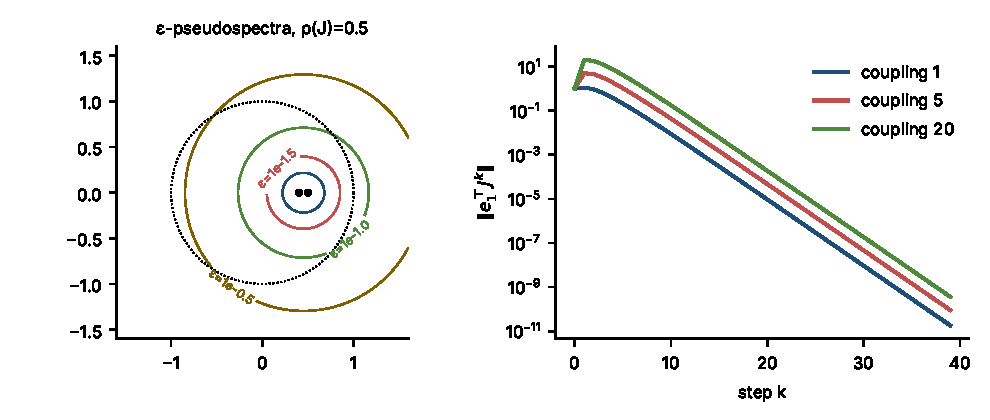
\includegraphics[width=0.95\textwidth]{figs/fig_pseudo.pdf}
\caption{Left: $\varepsilon$-pseudospectra of $J=\begin{psmallmatrix}0.5&5\\0&0.4\end{psmallmatrix}$; the eigenvalues (dots) are well inside the unit circle (dotted), but the $\varepsilon=10^{-1}$ contour reaches beyond it. Right: price-row gain $\|e_1^\top J^k\|$ for couplings 1, 5 and 20.}\label{fig:pseudo}
\end{figure}

\begin{lemma}[No amplification without depth; companion paper]\label{lem:cm}
In the cohort economy \eqref{eq:J} with nonnegative weights and $\rho(J)<1$, the price impulse response is a nonnegative mixture of decaying exponentials with total weight $\kappa$. It is completely monotone and peaks at the direct impact.
\end{lemma}

Lemma~\ref{lem:cm} is a negative result with a positive use. The cohort matrix \eqref{eq:J} is non-normal, yet its price output never amplifies. Non-normality is necessary for price amplification but not sufficient, and adaptive momentum feedback alone does not supply it. Section~\ref{sec:t6} shows that depth depletion does.

\subsection{Multi-asset coupling}

Market makers trade many correlated instruments. Let $x_t\in\R^d$ be pricing errors and $u_t\in\R^d$ flows, with $x_{t+1}=Ax_t+Ku_t+w_{t+1}$, $A={\rm diag}(a_1,\ldots,a_d)$, a cross-impact matrix $K$, and momentum flow $y_{t+1}=(I-H)y_t+Hx_{t+1}$, $u_t=Qy_t$. The stacked Jacobian is
\begin{equation}\label{eq:Jmulti}
J_{\rm multi}=\begin{pmatrix}A&KQ\\ HA&I-H+HKQ\end{pmatrix}\in\R^{2d\times2d}.
\end{equation}

\begin{proposition}[Directed cross-impact shrinks the safe radius]\label{prop:multi}
Suppose a leader--satellite structure ($K_{12}=0$, $K_{21}\ge0$) with $A,Q,K\ge0$ entrywise, $H\in(0,1)^d$, stable diagonal blocks and a fixed output $C\ge0$. Let $J_{\rm diag}$ be the decoupled Jacobian with $K_{21}=0$. Then every power $J_{\rm multi}^t$ is entrywise non-decreasing in $K_{21}$, so $M_C(J_{\rm multi})\ge M_C(J_{\rm diag})$ and $r^*_{\rm exact}(J_{\rm multi})\le r^*_{\rm exact}(J_{\rm diag})$; likewise $\mathcal K(J_{\rm multi})\ge\mathcal K(J_{\rm diag})$.
\end{proposition}

The proposition concerns nonnegative downstream coupling under a fixed output and shock set. Hedged or signed monetary outputs need separate treatment, and the size of the effect requires an empirical calibration we do not provide. Persistence and transient amplification are nevertheless different things: in a network of identical cohort economies coupled by symmetric nonnegative cross-impact, which stays symmetric in suitable coordinates, cross-impact of $0.05$ raises the spectral radius from $0.822$ ($d=1$) to $0.973$ ($d=10$) while the Kreiss constant stays at one (\texttt{recompute\_oct20.py}). Directed coupling, as in Proposition~\ref{prop:multi}, is what turns persistence into amplification.
\section{When does a book amplify? An exact condition}\label{sec:t6}

Transient path risk takes two forms, and the distinction organizes both the theory and the evidence. The first is \emph{peak overshoot}, a response that rises above its direct impact; Theorem~\ref{thm:t6} shows that it requires depth depletion to outweigh impact-weighted reversion. The second is \emph{cumulative amplification}, a summed response $S$ much larger than direct impact; Proposition~\ref{prop:sum} shows that it arises without any depletion whenever reversion is slow relative to impact and momentum. The guard of Section~\ref{sec:guard} bounds the second. The data of Sections~\ref{sec:depth}--\ref{sec:thin} show no peak overshoot in crypto books, even though flow depletes the side it hits on a fixed price grid, and they support the second form in thin books.

\subsection{A book with depletion and refill}
Let $x_t$ be the price displacement, $d_t$ the signed depth imbalance (bid minus ask depth near the mid, relative to total) and $u_t$ signed order flow. Flow moves the price directly and depletes one side of the book, which refills at rate $r$; depth imbalance moves the price:
\begin{align}
x_t &= a\,x_{t-1} + \varphi\,d_{t-1} + \kappa\,u_t, \label{eq:x}\\
d_t &= (1-r)\,d_{t-1} + \varepsilon\,u_t, \label{eq:d}
\end{align}
with $\kappa>0$, $a\in[0,1)$ and $r\in(0,1]$. Write $b=1-r$. With the sign convention $d=(B-A)/(B+A)$, a buy that consumes ask depth raises $d$, so $\varepsilon>0$ means \emph{depletion} of the side that is hit, and $\varphi>0$ means that a bid-heavy book pushes the price up. The impulse response to a unit flow shock at $t=0$ is $h_0=\kappa$ and
\begin{equation}\label{eq:rec}
h_k=a\,h_{k-1}+\varphi\varepsilon\,b^{k-1},\qquad k\ge1.
\end{equation}

\begin{definition}
The book \emph{amplifies} if $\max_kh_k>h_0$: the price keeps moving in the direction of the shock after the shock has passed.
\end{definition}

\subsection{The two-state theorem}

\begin{theorem}[Amplification condition]\label{thm:t6}
In model \eqref{eq:x}--\eqref{eq:d}, the book amplifies if and only if
\[
C_2\equiv\varphi\varepsilon-(1-a)\kappa>0 .
\]
When $C_2\le0$ the response peaks at impact, $\max_kh_k=\kappa$.
\end{theorem}

\begin{proof}
\emph{If.} $h_1-h_0=a\kappa+\varphi\varepsilon-\kappa=C_2>0$.

\emph{Only if.} Suppose $C_2\le0$. If $\varphi\varepsilon<0$, then by \eqref{eq:rec} $h_k=a^k\kappa+\varphi\varepsilon\sum_{j<k}a^{k-1-j}b^j\le a^k\kappa\le\kappa$. If $\varphi\varepsilon\ge0$, let $\Delta_k=h_k-h_{k-1}$. Then $\Delta_1=C_2\le0$ and, from \eqref{eq:rec},
\[
\Delta_{k+1}=a\Delta_k+\varphi\varepsilon(b^{k}-b^{k-1})=a\Delta_k-\varphi\varepsilon\,r\,b^{k-1}\le a\Delta_k .
\]
By induction $\Delta_k\le0$ for all $k$, so $h$ is non-increasing and peaks at $h_0=\kappa$.
\end{proof}

\paragraph{Interpretation.} The left side $\varphi\varepsilon$ is the extra price pressure that a unit of flow creates one period later through the book it leaves behind. The right side $(1-a)\kappa$ is the part of the direct impact that reverts in one period. The book amplifies exactly when the depth channel adds more than mean reversion removes. Refill $r$ does not enter the condition; it governs how long an overshoot lasts.

\begin{proposition}[Shape of the overshoot]\label{prop:shape}
For $a\neq b$ the response is $h_k=Aa^k+Bb^k$ with $B=\varphi\varepsilon/(b-a)$ and $A=\kappa-B$. When the book amplifies ($\varphi\varepsilon>(1-a)\kappa$):
\begin{enumerate}[label=(\roman*)]
\item In the interior regime $0<a\neq b<1$ with $AB<0$, the continuous profile $k\mapsto Aa^k+Bb^k$ on $k\ge0$ has a unique stationary point at
\[
k^*=\frac{\log\bigl(-A\log a/(B\log b)\bigr)}{\log(b/a)},
\]
so the discrete peak lag is $\lfloor k^*\rfloor$ or $\lceil k^*\rceil$ when $k^*\ge1$, and is $1$ when $k^*<1$ (because $h_1>h_0$).
\item On the boundary cases: if $a=0$ and $b\in(0,1)$, then $h_0=\kappa$ and $h_k=\varphi\varepsilon b^{k-1}$ for $k\ge1$, which peaks at $k=1$; if $0<a<b<1$ and $A\le0$, then $h'(k)$ turns negative at $k^*\le1$ so the discrete peak is at $k=1$; and in the confluent limit $a=b\in(0,1)$, $h_k=(\kappa+\varphi\varepsilon k/a)a^k$ with unique continuous peak at $k^*=1/\log(1/a)-\kappa a/(\varphi\varepsilon)$.
\end{enumerate}
In all cases with $a\in[0,1)$ and $r=1-b\in(0,1)$, the cumulative response is $\sum_{k\ge0}h_k=\kappa/(1-a)+\varphi\varepsilon/[(1-a)r]$, and faster refill $r$ lowers both the peak and the cumulative response.
\end{proposition}

We verify Theorem~\ref{thm:t6} in 1,995 random parameter draws and the refill comparative static in 565 amplifying draws, with no exceptions. The peak lag lies in the stated bracket in all of 150{,}039 amplifying draws; it is not always the integer nearest to $k^*$, which an earlier version claimed and which fails in 15\% of draws (\texttt{recompute\_audit.py}). Figure~\ref{fig:t6} illustrates the four cases.

\begin{figure}[t]\centering
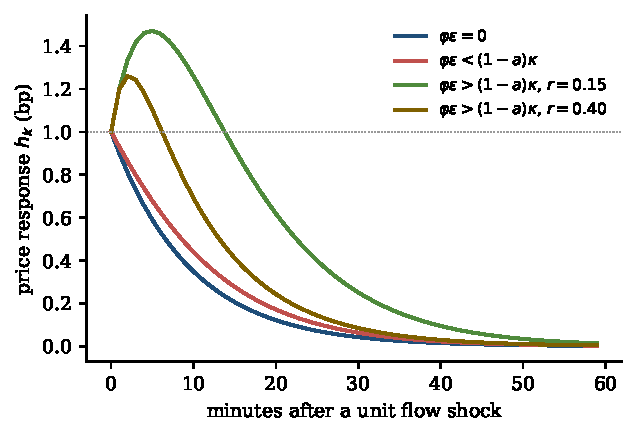
\includegraphics[width=0.6\textwidth]{figs/fig_t6.pdf}
\caption{Illustrative impulse responses of model \eqref{eq:x}--\eqref{eq:d} ($a=0.9$, $\kappa=1$, $\varepsilon=0.1$). The response overshoots only when $\varphi\varepsilon>(1-a)\kappa$; faster refill $r$ lowers the overshoot. Parameters are illustrative, not estimates.}\label{fig:t6}
\end{figure}

\subsection{Momentum traders}

Add momentum traders whose flow $f_t=(1-\eta)f_{t-1}+\eta q\,x_{t-1}$ enters both \eqref{eq:x} and \eqref{eq:d} alongside $u_t$.

\begin{proposition}[One-period amplification margin]\label{prop:t6m}
Let $C_3\equiv\varphi\varepsilon+\kappa^2\eta q-(1-a)\kappa$. Then $h_1-h_0=C_3$, so $C_3>0$ implies that the book amplifies.
\end{proposition}

\begin{proof}
With a unit shock at $t=0$, $x_0=\kappa$, $d_0=\varepsilon$ and $f_1=\eta q\kappa$, so $h_1=a\kappa+\varphi\varepsilon+\kappa^2\eta q$.
\end{proof}

With two slow modes the converse fails, and no condition on the one-period margin is exact. Three results describe what can be said instead.

\begin{theorem}[Momentum alone cannot make a stable book amplify]\label{thm:nomom}
Suppose $\varphi\varepsilon=0$ and $q\ge0$, and the system is stable. Then $h_k\le\kappa\,\rho^k<\kappa$ for every $k\ge1$, where $\rho<1$ is the spectral radius. In particular $C_3<0$.
\end{theorem}

\begin{proof}
Without the depth channel the state $(x_t,f_t)$ evolves by $M=\begin{psmallmatrix}a+\kappa\eta q&\kappa(1-\eta)\\ \eta q&1-\eta\end{psmallmatrix}$, which is entrywise nonnegative, and $h_k=\kappa(M^k)_{11}$. The off-diagonal product is nonnegative, so the eigenvalues are real, and by the Perron--Frobenius theorem $\lambda_2\le m_{11}\le\lambda_1=\rho$. Writing $(M^k)_{11}=c_1\lambda_1^k+c_2\lambda_2^k$ with $c_1=(m_{11}-\lambda_2)/(\lambda_1-\lambda_2)\in[0,1]$ and $c_2=1-c_1$ gives $(M^k)_{11}\le\rho^k$. Since $m_{11}\le\rho<1$, $C_3=\kappa(m_{11}-1)<0$.
\end{proof}

\begin{theorem}[A sufficient condition for no overshoot]\label{thm:noover}
For any signs of $\varphi$, $\varepsilon$ and $q$, if
\[
\bar C_3\equiv|\varphi\varepsilon|\Bigl(1+\frac{\kappa|q|}{r}\Bigr)+\kappa^2|q|-(1-a)\kappa\;\le\;0,
\]
then $\sup_k|h_k|=\kappa$: the response never exceeds its impact in either direction. When $\varphi\varepsilon\ge0$ and $q\ge0$, $C_3>0\Rightarrow$ amplification $\Rightarrow\bar C_3>0$.
\end{theorem}

\begin{proof}
Suppose $|x_j|\le\kappa$ for $j<k$. Then $|f_j|\le|q|\kappa$ for $j\le k$ and $|d_{k-1}|\le|\varepsilon|\bigl(b^{k-1}+\sum_{j\ge1}b^{k-1-j}|q|\kappa\bigr)\le|\varepsilon|(1+|q|\kappa/r)$, so $|x_k|\le a\kappa+|\varphi\varepsilon|(1+\kappa|q|/r)+\kappa^2|q|\le\kappa$. Induction from $x_0=\kappa$ completes the proof.
\end{proof}

\begin{remark}[Counterexamples to an exact one-period condition]\label{rem:counter}
Between $C_3$ and $\bar C_3$ the sign of $C_3$ does not decide. With $\kappa=1$, $a=0.98526$, $\varphi=0.7409$, $\varepsilon=0.01183$, $r=0.03436$, $\eta=0.5092$ and $q=0.01127$ (all channels reinforcing, $\rho=0.9995$), $C_3=-0.00024$ but the response peaks at lag 60 at $1.092\kappa$. With replenishment ($\varphi=2.614$, $\varepsilon=-0.405$, $a=0.9426$, $r=0.033$, $\eta=0.0016$, $q=0.0785$, $\rho=0.998$), $C_3=-1.11$ yet the response oscillates to $9.2\kappa$ at lag 90. In a search over 400{,}000 parameter draws such cases occur only near the stability boundary or with slow refill and slow momentum.
\end{remark}

\begin{proposition}[Summed response in closed form]\label{prop:sum}
Let $\tilde\kappa=\kappa+\varphi\varepsilon/r$ (long-run impact: direct plus depth) and $m=1-a$ (reversion). In the stable three-state model,
\[
S\equiv\sum_{k\ge0}h_k=\frac{\tilde\kappa}{m-q\tilde\kappa},
\]
and when $\varphi\varepsilon\ge0$ and $q\ge0$ the system is stable only if $m>q\tilde\kappa$. When all $h_k\ge0$, $S$ is the summed absolute response that enters the guard of Section~\ref{sec:guard}.
\end{proposition}

\begin{proof}
$S=e_1^\top(I-M_3)^{-1}(\kappa,\varepsilon,0)^\top$ with $M_3$ the transition matrix of $(x,d,f)$. Direct computation gives $\det(I-M_3)=\eta\,[\,r(m-\kappa q)-\varphi\varepsilon q\,]$ and the stated ratio; the formula matches the simulated sums to a relative error of $7\times10^{-14}$ in 3{,}000 stable draws.
\end{proof}

Cumulative transient risk is long-run impact divided by reversion net of momentum. Two practical consequences follow. First, the statistic that matters for losses is the summed response, which grows without bound as reversion falls to $q\tilde\kappa$, even when no single lag overshoots (Theorem~\ref{thm:nomom}). Second, $C_3$ is best read as a one-period amplification margin: it moves with $m$, $q$ and $\tilde\kappa$ in the same direction as $S$ and is what we estimate in Sections~\ref{sec:depth} and~\ref{sec:thin}. Both statistics are invariant in sign to rescaling flow.

\section{An identification-free pre-trade guard}\label{sec:guard}

\subsection{The quantity gate}
Observable dynamics are $z_{j+1}=Jz_j+Hv_j$ with loss output $l_t=Cz_t$ and impulse coefficients $g_m=c^\top_{\rm price}J^mH$. Let $b_t=CJ^tz_0$ be the drift from past flow, $G_{{\rm single},t}=\max_{m<t}|g_m|$ the single-shock peak gain up to $t$, and $G_{{\rm cum},t}=\sum_{m=0}^{t-1}|g_m|$ the cumulative convolution gain for repeated per-period trades $|v_j|\le V$. Superposition gives, under a reserve $L_{\rm other}$ and execution cost $c_{\rm exec}$, the sharp repeated-trade allowance (and its single-impulse counterpart)
\begin{equation}\label{eq:gate}
\begin{aligned}
V^*_{\rm repeated} &= \min_{t:\,G_{{\rm cum},t}+c_{\rm exec}>0}\frac{B-L_{\rm other}-|b_t|}{G_{{\rm cum},t}+c_{\rm exec}}, \qquad\bar R=V^*_{\rm repeated}/\tau, \\[2pt]
V^*_{\rm single} &= \min_{t:\,G_{{\rm single},t}+c_{\rm exec}>0}\frac{B-L_{\rm other}-|b_t|}{G_{{\rm single},t}+c_{\rm exec}}
\end{aligned}
\end{equation}
over a window of $\tau$ seconds. Using $G_{{\rm single},t}$ in place of $G_{{\rm cum},t}$ when trades repeat every period under-states worst-case cumulative exposure whenever multiple lags are nonzero. The gate needs only impulse coefficients and the current drift.

\subsection{Maximality}
A dealer with inventory $I$ chooses an admission level $\alpha\in[0,1]$ (the fraction of incoming algorithmic flow it accepts, or the depth it quotes). The closed-loop operator is $J(\alpha)=J_0+\alpha B_F$ with price impulse response $g_k(\alpha)$. Shocks satisfy $|u_t|\le\bar u$. Over horizon $H$ the price change is $\sum_{k<H}g_k(\alpha)u_{t-k}$, and the dealer has a loss budget $\mathcal B$.

\begin{theorem}[Summed-gain guard is maximal]\label{thm:guard}
The worst-case loss over horizon $H$ is
\[
L_{\max}(\alpha)=|I(\alpha)|\,\bar u\sum_{k<H}|g_k(\alpha)|.
\]
Hence the guard ``admit $\alpha$ iff $L_{\max}(\alpha)\le\mathcal B$'' is necessary and sufficient for bounded-shock solvency: it admits every safe $\alpha$ and no unsafe one. Replacing $\sum_k|g_k|$ by $\max_k|g_k|$ can admit unsafe levels; replacing it by $H\max_k|g_k|$ is safe but conservative.
\end{theorem}

\begin{proof}
By H\"older's inequality $|\sum_kg_ku_{t-k}|\le\bar u\sum_k|g_k|$, with equality for $u_{t-k}=\bar u\,{\rm sign}(g_k)$, which is admissible. Multiplying by $|I(\alpha)|$ gives $L_{\max}$, so the admission set equals the safe set. Since $\max_k|g_k|\le\sum_k|g_k|\le H\max_k|g_k|$, the peak guard under-states loss and the $H$-scaled guard over-states it.
\end{proof}

The worst-case identity in Theorem~\ref{thm:guard} is not new as mathematics: the induced $\ell_\infty$ gain of a linear convolution operator is the $\ell_1$ norm of its kernel, the fact on which $\ell_1$-optimal control of persistent bounded disturbances is built \citep{vidyasagar1986,dahleh1987,dahleh1995}. We use it rather than claim it. The finance content lies elsewhere: the dealer's admission level changes the operator itself, so the guard is a rule over an action set rather than a controller design; the bound is carried through margin, hedging and fill accounting (Theorem~\ref{thm:forward}); its single input is invariant to how the unobserved traders are split into cohorts and is identified from prices (Propositions~\ref{prop:invariance} and~\ref{prop:bridge}); the peak-response and eigenvalue rules it is compared with are the ones closest to current supervisory practice; and the same statistic prices the corrective rebate in equilibrium (Proposition~\ref{prop:equil}).

Numerically, the guard coincides with a brute-force adversary's maximal safe $\alpha$ in 200 of 200 random states. The peak-gain guard admitted an unsafe level in 2,000 of 2,000 states, the $H$-scaled guard was conservative in all 2,000, and $L_{\max}$ was non-decreasing in $\alpha$ in all 2,000, so the admission set was an interval in these examples.

\subsection{Computability: a finite-horizon certificate}

\begin{lemma}[Contraction-block tail bound]\label{lem:tail}
Let $\rho(J(\alpha))<1$. Suppose that at horizon $H$ there is a block length $H_0\le H$ with $q(\alpha)\equiv\|J(\alpha)^{H_0}\|_2<1$, and let $\bar M_{H_0}(\alpha)=\max_{0\le r<H_0}\|c^\top_{\rm price}J(\alpha)^r\|_2$ and $M_{C,H}(\alpha)=\max_{k\le H}\|c^\top_{\rm price}J(\alpha)^k\|_2$. Then
\begin{align}
\sup_{k\ge0}\|c^\top_{\rm price}J(\alpha)^k\|_2&\le\max\Bigl(M_{C,H}(\alpha),\ \bar M_{H_0}(\alpha)q(\alpha)^{\lfloor(H+1)/H_0\rfloor}\Bigr),\label{eq:tail}\\
G_{{\rm cum},\infty}(\alpha)&\le G_{{\rm cum},H}(\alpha)+\frac{\bar M_{H_0}(\alpha)H_0\,q(\alpha)^{\lfloor(H+1)/H_0\rfloor}}{1-q(\alpha)}.\notag
\end{align}
\end{lemma}

\begin{proof}
Write any $k>H$ as $k=mH_0+r$ with $m\ge\lfloor(H+1)/H_0\rfloor$ and $0\le r<H_0$. Submultiplicativity gives $\|c^\top J^k\|\le\|c^\top J^r\|\,\|J^{H_0}\|^m\le\bar M_{H_0}q^m$. Taking the supremum and summing the geometric tail gives \eqref{eq:tail}.
\end{proof}

The certificate turns an infinite-horizon supremum into a finite computation with a verified remainder. If the second term in the maximum is below $M_{C,H}$, truncation at $H$ is exact.

\subsection{Robustness to estimation error}

\begin{theorem}[Robust gain]\label{thm:robust}
Let $M=\sup_k\|J^k\|$ and $S=\sum_k\|J^k\|$. If $\|E\|\le\epsilon$ and $\epsilon S<1$, then $\sup_k\|(J+E)^k\|\le M/(1-\epsilon S)$.
\end{theorem}

\begin{proof}
Let $P_k=(J+E)^k$. Expanding, $P_k=J^k+\sum_{j<k}J^{k-1-j}EP_j$. With $m_k=\|P_k\|$, $m_k\le M+\epsilon\sum_{j<k}\|J^{k-1-j}\|m_j\le M+\epsilon S\max_{j<k}m_j$. Since $m_0=1\le M$, induction gives $m_k\le M/(1-\epsilon S)$ for all $k$.
\end{proof}

The bound held in all 30,000 random perturbations of 100 non-normal operators, with median tightness $0.50$ (realized gain over bound; maximum $0.57$). In a simulated window estimator of the kind used in Section~\ref{sec:spot} (600 transitions), a residual-bootstrap 95\% ball for the operator covered the true $J$ in $94.7\%$ of 300 replications, with median radius $0.086$; but $\epsilon S<1$ held in only $8\%$ of windows. The certificate is valid but often unavailable at realistic sample sizes; longer windows or pooled estimates are needed to use it in practice.

\begin{proposition}[No identification needed; numerical]\label{prop:bridge}
In a two-cohort economy with rates $0.7\pm\Delta$, the relative error of the estimated summed gain is flat in $\Delta$ (log--log slope $-0.15$), while the error of the cohort weights grows as $\Delta^{-3.07}$.
\end{proposition}

The guard needs the summed gain, which is cheap to estimate and invariant to cohort splitting (Proposition~\ref{prop:invariance}); it does not need the algorithms' identities, which are expensive \citep{niroula2026}.

\subsection{A calibrated illustration}\label{sec:calib}

How much does the choice between peak and summed guards matter in a real book? We compute the three-state impulse response at the median estimates of Section~\ref{sec:depth} (all training days and high-volatility days) and at a hypothetical book in which flow depletes the side it hits ($\varepsilon=+0.02$, other parameters at their high-volatility medians), Figure~\ref{fig:calib} and Table~\ref{tab:calib}.

\begin{figure}[t]\centering
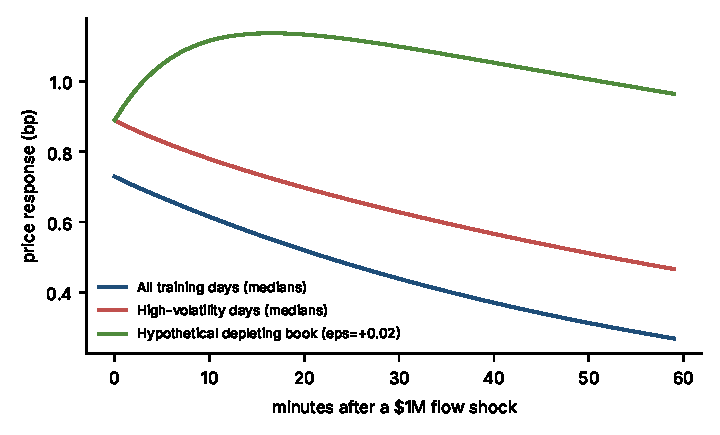
\includegraphics[width=0.62\textwidth]{figs/fig_calib.pdf}
\caption{Price response to a \$1M flow shock at the median depth estimates and in a hypothetical depleting book. Computed from the estimates of Table~\ref{tab:d3}.}\label{fig:calib}
\end{figure}

\begin{table}[t]\centering\small
\begin{threeparttable}
\caption{Peak versus summed gain at calibrated parameters}\label{tab:calib}
\setlength{\tabcolsep}{4pt}
\begin{tabular}{p{0.2\textwidth}ccccccc}
\toprule
Book & $C_3$ & Peak (min) & $\sum_{k<15}|g_k|$ & $\sum_{k<60}|g_k|$ & Sum/peak & Cap, peak & Cap, sum\\
\midrule
All days (medians) & $-0.013$ & 0.73 (0) & 9.73 & 27.67 & 13.3 & \$274M & \$21M\\
High-vol.\ days (medians) & $-0.014$ & 0.89 (0) & 12.17 & 38.71 & 13.7 & \$225M & \$16M\\
Depleting book ($\varepsilon=0.02$) & $+0.042$ & 1.14 (17) & 15.85 & 63.69 & 14.0 & \$176M & \$13M\\
\bottomrule
\end{tabular}
\begin{tablenotes}\footnotesize\item Gains in bp per \$1M of flow; sum/peak at 15 minutes. Inventory cap under a peak guard and under the summed guard, for a loss budget of \$100,000, an illustrative shock bound of \$5M of flow per minute and a 15-minute horizon. From \texttt{calib\_guard.py}, using the medians of Table~\ref{tab:d3}.\end{tablenotes}
\end{threeparttable}
\end{table}

The result is striking even though BTCUSDT does not amplify. Because price impact is persistent ($\hat a\approx0.97$ per minute), the summed gain over 15 minutes is about 13 times the peak. A guard calibrated to the peak would admit inventory about 13 times larger than is safe against a sustained adversarial flow of the declared size. Amplification makes this worse (the depleting book peaks 17 minutes after the shock), but persistence alone already makes peak-based limits unsafe. This is the practical content of Theorem~\ref{thm:guard} for this market.

\subsection{Two deployment modes}

\begin{enumerate}[label=\textbf{Mode \Alph*.},leftmargin=*]
\item \emph{An individual dealer.} A price-taking market maker with a small share of aggregate depth scales its own quote size by $\alpha$. This scales its passive fill intake but leaves aggregate depth, impact and the market operator unchanged.
\item \emph{A venue or sponsoring broker.} A gate at a matching engine or a market-access gateway (the setting of Rule 15c3-5) admits a fraction $\alpha$ of incoming aggressive algorithmic flow while resting depth stays posted. The operator becomes $J(\alpha)=A_0+\alpha B_F$.
\end{enumerate}

\paragraph{Algorithm (pre-trade guard).} At each step, using only pre-shock information:
\begin{enumerate}[itemsep=1pt]
\item For each $\alpha$ on a grid $\mathcal A=\{0,0.025,\ldots,1\}$, compute $\rho(J(\alpha))$, the peak and summed gains $M_{C,H}(\alpha)$ and $G_{{\rm cum},H}(\alpha)$, and the tail certificate of Lemma~\ref{lem:tail}; if an operator confidence radius $\epsilon$ is available, inflate by Theorem~\ref{thm:robust}.
\item Compute post-hedge and worst-case post-fill inventory, hedging cost and the post-fill margin increment.
\item Admit the largest $\alpha\in\mathcal A$ that satisfies the solvency inequalities of Theorem~\ref{thm:forward}; if none does, set $\alpha=0$, flag that no safe action exists, and trigger inventory reduction.
\end{enumerate}
For low-dimensional $J$ the grid evaluation is a sequence of matrix--vector products; execution takes well under one millisecond in compiled code, which we regard as an engineering detail rather than a result.

\subsection{Balance-sheet solvency}

\begin{theorem}[Conditional bounded-shock forward solvency]\label{thm:forward}
Consider a dealer with cash $K_t$, inventory $I_t$, mark $p_t$, equity $E_t=K_t+I_tp_t$, maintenance margin $MM_t=\max(0,\mu|I_t|p_t-c_0)$ and remaining buffer $B_{{\rm rem},t}=E_t-MM_t$, a safety reserve $R_{\rm safe}$, a hedge $\Delta I^{\rm hedge}_t(\alpha)$ with cost $C_{{\rm hedge},t}(\alpha)$, worst-case passive fills $\Delta I^{\rm fill}_{\max,t}(\alpha)$ with margin increment $C_{{\rm fill},t}(\alpha)$, and declared one-step and cumulative shock envelopes $\bar u_{{\rm step},t}\le\bar u_{{\rm cum},t}$. Let $|I^{\rm post}_{t+1}(\alpha)|=|I_t+\Delta I^{\rm hedge}_t(\alpha)|+\Delta I^{\rm fill}_{\max,t}(\alpha)$. Suppose the guard admits $\alpha_t$ only if
\begin{equation}\label{eq:guardineq}
|I^{\rm post}_{t+1}(\alpha_t)|(1+\mu)\Bigl(M_{C}(\alpha_t)\|z_t\|_2+s(\alpha_t)G_{\rm cum}(\alpha_t)\bar u_{{\rm cum},t}\Bigr)+C_{{\rm hedge},t}(\alpha_t)+C_{{\rm fill},t}(\alpha_t)+R_{\rm safe}\le B_{{\rm rem},t},
\end{equation}
where $s(\alpha)$ scales admitted shocks. Then for every disturbance path within the declared envelopes, the buffer after the step is at least $R_{\rm safe}$; by induction, solvency holds at every step at which an admissible $\alpha$ exists. At $\alpha=0$ the one-step admissible shock is
\[
\bar u_{{\rm adm},t}=\frac{B_{{\rm rem},t}-R_{\rm safe}-|I_t|(1+\mu)\|z_t\|_2}{|I_t|(1+\mu)} .
\]
The condition is sufficient over the whole disturbance ball. It is also necessary when the current state contributes no drift ($z_t=0$), because the shock term is then attained by adversarially signed disturbances; with $z_t\neq0$ the drift term $M_C\|z_t\|_2$ is an upper bound and the condition may be conservative. The admissible shock at $\alpha=0$ assumes, as in the cohort economy (Lemma~\ref{lem:cm}), that the price-row gain without admitted flow is $M_C(0)=1$.
\end{theorem}

Two features matter. The guard accounts for the inventory the dealer will hold after hedging and after worst-case fills, not only current inventory, and it never claims safety on an infeasible state: if no $\alpha$ satisfies \eqref{eq:guardineq}, it halts new fills and flags the state, because pre-existing inventory can still breach margin on a large adverse jump. In a constructed scenario ($E_0=10{,}000$, $I_0=-2{,}000$ at $P^*=100$, Tier-2 margin with $\mu=0.005$, buffer $9{,}050$ and reserve $950$), the admissible shock at $z_0=0$ is $8{,}100/2{,}010=4.03$ per unit, and an adversarial move of $4.05$ violates the reserve.

\begin{proposition}[When the guard beats an eigenvalue rule]\label{prop:dominance}
Let an eigenvalue guard admit $\alpha_\rho=\max\{\alpha:\rho(J(\alpha))\le\bar\rho\}$, and suppose the state is feasible for the summed-gain guard, which then admits at least $\alpha=0$.
\begin{enumerate}[label=(\roman*)]
\item Over the Euclidean state ball $\{\tilde z_t:\|\tilde z_t\|_2\le\|z_t\|_2\}$ and one-step shock envelope $|u_{t+1}|\le\bar u_{{\rm step},t}$, the eigenvalue guard violates the robust solvency bound \eqref{eq:guardineq} if and only if
\[
M_C(\alpha_\rho)\|z_t\|_2+s(\alpha_\rho)|g_0(\alpha_\rho)|\bar u_{{\rm step},t}\;>\;\frac{B_{{\rm rem},t}-R_{\rm safe}-C_{{\rm hedge},t}(\alpha_\rho)-C_{{\rm fill},t}(\alpha_\rho)}{|I^{\rm post}_{t+1}(\alpha_\rho)|(1+\mu)} .
\]
\item At a specific state $z_t$, the eigenvalue guard admits an exact reachable one-step breach that the summed-gain guard prevents if and only if the exact reachable price excursion $|c^\top_{\rm price}J(\alpha_\rho)z_t|+s(\alpha_\rho)|g_0(\alpha_\rho)|\bar u_{{\rm step},t}$ exceeds the right-hand side above.
\end{enumerate}
\end{proposition}

The eigenvalue rule fails exactly when the transient gain at its admitted level exceeds the loss the balance sheet can absorb, which Proposition~\ref{prop:blind} shows can happen at any spectral threshold.

\begin{proposition}[Strategic re-optimization reinforces the guard]\label{prop:lucas}
Suppose cohorts re-optimize their steady-state Kalman gains when the venue throttles admission, and throttling scales the variance of execution-driven innovations as $\sigma_\zeta^2(\alpha)=\alpha^2\sigma_{\zeta,0}^2$ while measurement noise $\sigma_\nu^2>0$ is unchanged. Then the optimal gain $\eta^*(\alpha)$ is strictly increasing in $\alpha$, so throttling lowers every cohort's adaptation rate. If the transient gain is non-decreasing in the adaptation rates, then $M_C(J(\alpha,\eta^*(\alpha)))\le M_C(J(\alpha,\eta^*(1)))$: re-optimization does not undo the guard.
\end{proposition}

The first statement is a property of the Riccati root; the second is conditional on monotonicity of the gain in $\eta$, which we check numerically. Across 3{,}000 stable draws of the three-state book with momentum (adaptation rates on a grid from 0.05 to 0.95), the peak response is non-decreasing in $\eta$ in 98.8\% of draws and in 99.9\% of those with trend-following cohorts ($q>0$); the summed absolute response is non-decreasing in 93\% of draws with $q>0$ but decreasing when cohorts are contrarian ($q<0$). For trend-following cohorts, the case the filtering microfoundation produces, re-optimization therefore reinforces the guard in almost every case we drew; the signed sum $S$ of Proposition~\ref{prop:sum} does not depend on $\eta$ at all (\texttt{recompute\_oct20.py}). A manipulator who instead increases order size to offset throttling enlarges the shock envelope and drives $\alpha$ toward zero.
\section{Who provides reversion? An equilibrium}\label{sec:equil}

Proposition~\ref{prop:sum} says that transient risk is governed by one ratio, $S=\tilde\kappa/(m-q\tilde\kappa)$. Its ingredients are chosen by market participants: dealers decide how hard to lean against price displacements, which sets reversion $m$, and momentum traders decide how strongly to chase them, which sets $q$. This section asks whether those choices are efficient.

\subsection{Setup}
There are $N$ dealers. Dealer $i$ supplies reversion intensity $s_i\ge0$ by absorbing order flow against the displacement, so $m=m_0+\sum_is_i$, where $m_0$ is reversion supplied by other means. Leaning earns a spread $v$ per unit of intensity at quadratic inventory cost, so the private value is $vs_i-\tfrac c2s_i^2$. By Theorem~\ref{thm:guard} the worst-case transient loss of a position of size $Q$ facing flow shocks bounded by $U$ is $QU\,S$, so we take aggregate expected tail loss to be $\Lambda S(m,q)$ with $\Lambda>0$. Dealers bear a share $\theta<N$ of it, so each bears $\theta/N$; leveraged users and their counterparties bear the rest. Momentum traders choose aggregate intensity $q$ with private value $bq-\tfrac e2q^2$ and bear none of the tail loss. Long-run impact $\tilde\kappa$ is taken as given.

\subsection{Results}

\begin{proposition}[Equilibrium transient risk]\label{prop:equil}
Let $g(m)\equiv-\partial S/\partial m=\tilde\kappa/(m-q\tilde\kappa)^2$.
\begin{enumerate}[label=(\roman*)]
\item \emph{Under-provision of reversion.} The symmetric Nash equilibrium solves $m-m_0=N v/c+\theta\Lambda g(m)/c$, the planner's optimum solves $m-m_0=N v/c+N\Lambda g(m)/c$, and $m^{\rm eq}<m^{\rm SP}$, so $S^{\rm eq}>S^{\rm SP}$.
\item \emph{Fewer dealers, more risk.} $\partial m^{\rm eq}/\partial N=(v/c)/(1-\theta\Lambda g'(m)/c)>0$, so equilibrium reversion rises and $S^{\rm eq}$ falls with the number of dealers.
\item \emph{Over-provision of momentum.} Momentum traders choose $q=b/e$; the planner chooses $q^{\rm SP}<b/e$, solving $b-eq=\Lambda\tilde\kappa^2/(m-q\tilde\kappa)^2$.
\item \emph{The corrective price is identified.} The first best for reversion is implemented by a rebate per unit of reversion
\[
\tau^*=\Bigl(1-\frac\theta N\Bigr)\Lambda\,g(m)=\Bigl(1-\frac\theta N\Bigr)\Lambda\,\frac{S^2}{\tilde\kappa},
\]
which depends on the market only through $S$ and $\tilde\kappa$.
\end{enumerate}
\end{proposition}

\begin{proof}
(i) Dealer $i$'s first-order condition is $v-cs_i+(\theta/N)\Lambda g(m)=0$; the planner's is $v-cs+\Lambda g(m)=0$. Summing over dealers gives the two fixed-point equations. The right-hand sides are decreasing in $m$ because $g$ is decreasing on $m>q\tilde\kappa$, and the planner's lies above the dealers' for every $m$ when $\theta<N$, so its crossing with the line $m-m_0$ lies to the right. (ii) follows by implicit differentiation, since $g'<0$. (iii) $\partial S/\partial q=\tilde\kappa^2/(m-q\tilde\kappa)^2>0$ is the marginal external cost of momentum that traders ignore. (iv) The rebate closes the wedge between the two first-order conditions, and $g=S^2/\tilde\kappa$ by Proposition~\ref{prop:sum}.
\end{proof}

At $v=0.002$, $c=0.5$, $\theta=0.3$, $\Lambda=10^{-4}$, $m_0=0.005$, $q=0.02$ and $\tilde\kappa=1$, equilibrium $S$ falls from 27.9 with one dealer to 6.8 with forty, and the planner's $S$ is 1.5--2.7 times lower throughout; the rebate computed from $S$ alone coincides with the first-order wedge to machine precision. With $m=0.03$, $b=0.3$ and $e=20$, momentum traders choose $q=0.015$ against a planner's $0.0062$.

\paragraph{Interpretation.} Reversion is a public good: each dealer who leans against a displacement lowers the tail exposure of every leveraged position in the market but is paid only for his own fills. Momentum is the mirror image. Part (iv) closes the loop with the guard: the policy price of the externality is a function of the same summed response that the guard bounds, and Propositions~\ref{prop:invariance} and~\ref{prop:bridge} show that this quantity is identified from public data without identifying the traders. A venue that rebates reversion in proportion to $S^2/\tilde\kappa$, or a supervisor that sets pre-trade limits by $S$, prices the externality with an observable.

\paragraph{What the data say about the model's predictions.} Part (ii) predicts that books with fewer dealers have higher $S$ because they supply less reversion. Depth is the closest proxy we observe for the number of liquidity providers. Across the three liquidity terciles of the 30 Binance perpetuals on training days, the summed response per dollar of flow rises steeply as depth falls (median $2{,}797$, $26{,}603$ and $39{,}329$ basis points per \$1M in the thick, mid and thin terciles; Spearman correlation with log depth $-0.94$), as (ii) predicts. The channel is not the one the model names, however: the unit-free gain multiple $S/|h_0|=1/(m-q\tilde\kappa)$, which isolates reversion net of momentum, is the same in all three terciles (medians $46.4$, $47.3$ and $46.9$; Spearman $-0.11$). Thinner books carry more cumulative risk because their impact $\tilde\kappa$ is larger, not because they revert more slowly. These comparisons were made after the fact (Part 13, \texttt{R2}), and depth is an imperfect proxy for dealer count, so a direct test needs data on liquidity-provider identities. The model's second prediction, that the dynamic balance forecasts tail losses where reversion is close to $q\tilde\kappa$, is what Section~\ref{sec:thin} tests.

\section{Information limits, safety certification, and the value of disclosure}\label{sec:flagship}

The guard of Section~\ref{sec:guard} requires the cumulative impulse response, whereas the companion paper establishes sharp limits on what finite market histories reveal about hidden adaptive cohorts. We now answer the unified question connecting the two papers: when the adaptive systems operating inside a market are only partially observed, what information is sufficient to certify safe trading decisions, what does that information cost, and how much financially valuable trading must be sacrificed when information is insufficient?

\subsection{An exact two-market ambiguity witness and information--safety impossibility}
Consider the positive-memory cohort economy $x_{t+1}=ax_t+\sum_{i=1}^K y_{i,t}+u_t$, $y_{i,t+1}=(1-\eta_i)y_{i,t}+\eta_i q_i x_t$ with $a=2/5=0.40$ and zero initial memory states. Table~\ref{tab:witness} and Figure~\ref{fig:flagship1} construct two asymptotically stable markets in exact rational arithmetic (test \texttt{T01}).

\begin{table}[t]\centering\small
\begin{threeparttable}
\caption{Two-market ambiguity witness (\texttt{T01})}\label{tab:witness}
\setlength{\tabcolsep}{6pt}
\begin{tabular}{lcc}
\toprule
Quantity & Market A ($K=1$) & Market B ($K=2$)\\
\midrule
Memory rates $\eta_i$ & $1/2=0.50$ & $1,\;1/20=0.05$\\
Feedback weights $q_i$ & $2/25=0.08$ & $1/50=0.02,\;2/5=0.40$\\
Total long-run feedback $Q=\sum_i q_i$ & $2/25=0.08$ & $21/50=0.42$\\
Early responses $(h_0,h_1,h_2)$ & $(1,\,2/5,\,1/5)$ & $(1,\,2/5,\,1/5)$\\
Lag-3 response $h_3$ & $29/250=0.116$ & $23/200=0.115$\\
Infinite-horizon cumulative gain $S_\infty$ & $25/13\approx 1.9231$ & $50/9\approx 5.5556$\\
Max.\ per-period shock $v_{\max}$ ($B=1,|I|=1$) & $13/25=0.52$ & $9/50=0.18$\\
\bottomrule
\end{tabular}
\begin{tablenotes}\footnotesize\item Verified in exact rational arithmetic and Lean~4. Both markets share $m_0=\sum_i\eta_i q_i=1/25=0.04$, so $h_0,h_1,h_2$ are identical.\end{tablenotes}
\end{threeparttable}
\end{table}

\begin{figure}[t]\centering
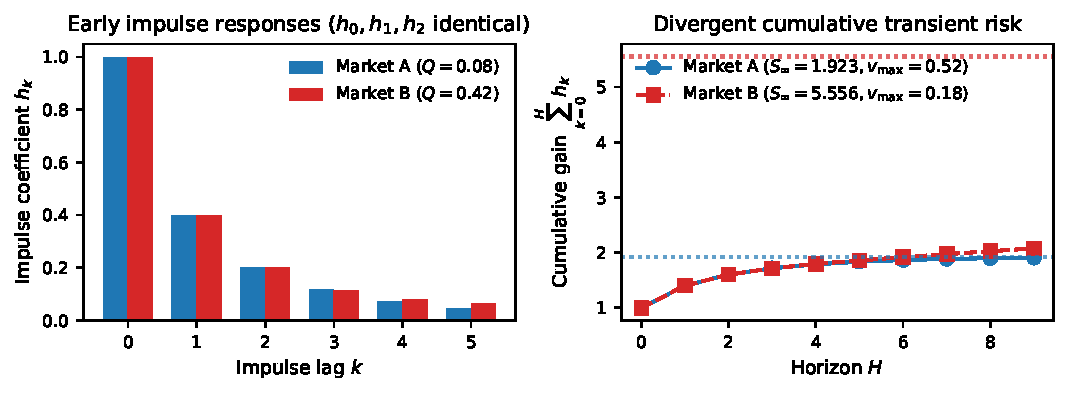
\includegraphics[width=0.88\textwidth]{figs/fig_flagship_1_witness.pdf}
\caption{Two-market ambiguity witness (\texttt{T01}): Market A and Market B produce identical impulse responses at lags $0,1,2$ and differ by only $10^{-3}$ at lag $3$, yet their infinite-horizon cumulative gains differ by nearly a factor of three ($1.9231$ vs.\ $5.5556$).}\label{fig:flagship1}
\end{figure}

\begin{theorem}[Unavoidable loss of safe trading capacity]\label{thm:flagship_A}
Suppose two candidate markets $\theta_0,\theta_1$ generate observation laws $P_0,P_1$ with total variation distance $d_{\rm TV}=\operatorname{TV}(P_0,P_1)$ and have maximum safe per-period allowances $0\le v_0<v_1$. For any data-dependent admission policy $A(D)\in[0,v_1]$ satisfying the level-$\beta$ safety requirement $P_0(A(D)>v_0)\le\beta$, the expected sacrificed safe trading capacity in Market 1 satisfies
\[
\mathbb E_1\bigl[v_1-A(D)\bigr]\;\ge\;(v_1-v_0)\bigl[1-\beta-d_{\rm TV}\bigr]_+ .
\]
For the witness pair of Table~\ref{tab:witness} under an observation contract that reveals $(h_0,h_1,h_2)$ ($d_{\rm TV}=0$, $v_0=9/50=0.18$, $v_1=13/25=0.52$) at $\beta=0.05$, any safe supervisor sacrifices at least $\mathbb E_A[0.52-A(D)]\ge 0.34\times 0.95=323/1000=0.323$ units of admissible capacity ($62.1\%$ of Market A's safe capacity).
\end{theorem}

\begin{proof}
Let $E=\{A(D)\le v_0\}$. Safety in Market 0 requires $P_0(E)\ge 1-\beta$, and the definition of total variation gives $P_1(E)\ge P_0(E)-d_{\rm TV}\ge 1-\beta-d_{\rm TV}$. Because $v_1-A(D)\ge 0$ everywhere and $v_1-A(D)\ge v_1-v_0$ on $E$, $\mathbb E_1[v_1-A(D)]\ge (v_1-v_0)P_1(E)$, yielding the bound.
\end{proof}

\subsection{Risk-specific identifiability and minimum observation budgets}
Unlike generic set-membership control \citep{vanwaarde2020}, the cohort recurrence links finite-lag impulse observations directly to Chebyshev--Markov--Stieltjes bounds on cumulative financial risk. By Proposition~6.1 of the companion paper, observing $(h_0,\ldots,h_L)$ up to lag $L\ge 2$ uniquely determines the open-loop memory moments $m_j=\sum_{i=1}^K w_i r_i^j$ ($0\le j\le d\equiv L-2$), where $w_i=\eta_i q_i\ge 0$ and $r_i=1-\eta_i\in[0,\bar r]$ ($\bar r=1-\eta_{\min}<1$).

\begin{theorem}[Sharp risk-specific identifiability envelope]\label{thm:flagship_B}
Let $\Theta(h_{0:L},\bar r)$ be the set of positive-memory markets compatible with $(h_0,\ldots,h_L)$ and retention bound $r_i\in[0,\bar r]$.
\begin{enumerate}[label=(\roman*)]
\item For $L=2$ ($d=0$, observing $m_0=h_2-ah_1$), the compatible long-run feedback sum $Q(\theta)=\sum_i w_i/(1-r_i)$ spans the exact interval $[Q_0^-(m_0),Q_0^+(m_0,\bar r)]=[m_0,\,m_0/(1-\bar r)]$. For $L=3$ ($d=1$, observing $(m_0,m_1)$), the sharp Markov--Krein envelope is
\[
Q_1^-(m_0,m_1)=\frac{m_0^2}{m_0-m_1}\;\le\;Q(\theta)\;\le\;m_0+\frac{m_1}{1-\bar r}=Q_1^+(m_0,m_1,\bar r),
\]
where Market A of Table~\ref{tab:witness} ($m_0=1/25,m_1=1/50$) attains $Q_1^-=2/25$ and Market B ($m_0=1/25,m_1=19/1000,\bar r=19/20$) attains $Q_1^+=21/50$.
\item Under $a+Q_d^+(m_{0:d},\bar r)<1$, the compatible worst-case loss for allowance $v$ is $R^+(h_{0:L},\bar r)=|I|v/(1-a-Q_d^+(m_{0:d},\bar r))$, so $v$ is certifiably safe ($R^+\le B$) if and only if $Q_d^+(m_{0:d},\bar r)\le 1-a-|I|v/B$, even when individual cohort parameters $(\eta_i,q_i)$ are unidentifiable.
\end{enumerate}
\end{theorem}

\begin{theorem}[Minimum observations for safe decisions vs.\ cohort identification]\label{thm:flagship_C}
Suppose an observer collects $N$ independent Gaussian impulse-response windows $\hat h^{(n)}=h_{0:L}(\theta)+\varepsilon^{(n)}$ with $\varepsilon^{(n)}\sim\mathcal N(0,\Sigma)$.
\begin{enumerate}[label=(\roman*)]
\item For any two markets $\theta_0,\theta_1$ with safe allowances $v_0<v_1$ and impulse difference $\Delta h=h_{0:L}(\theta_1)-h_{0:L}(\theta_0)$, keeping the expected capacity loss of a level-$\beta$ safe rule below $\epsilon(v_1-v_0)$ requires at least
\[
N\;\ge\;N_{\min}^{\rm safe}(\theta_0,\theta_1;\beta,\epsilon)\equiv\frac{4(1-\beta-\epsilon)_+^2}{\Delta h^\top\Sigma^{-1}\Delta h}.
\]
\item Certifying a safe allowance $v_{\rm target}$ with positive safety margin $\Delta_{\rm safe}=(1-a-Q(\theta^*))-v_{\rm target}>0$ requires lag horizon $L^*(\Delta_{\rm safe})=2+\lceil\log(m_0/((1-\bar r)^2\Delta_{\rm safe}))/\log(1/\bar r)\rceil$ and sample size $N=O(\sigma^2\Delta_{\rm safe}^{-2})$ independent of cohort separation $\Delta\eta$, whereas identifying individual cohort rates requires $N\asymp(\Delta\eta)^{-(4K-2)}$.
\end{enumerate}
\end{theorem}

\subsection{Statistically valid certification and the optimal uncertainty-aware guard}
When impulse responses are estimated from $N$ windows with covariance $\Sigma_N=\Sigma/N$, let $\mathcal C_\gamma(D)=\{\theta\in\Theta(\bar r):(\hat h_{0:L}-h_{0:L}(\theta))^\top\Sigma_N^{-1}(\hat h_{0:L}-h_{0:L}(\theta))\le\chi^2_{L+1,1-\gamma}\}$ denote the $(1-\gamma)$ confidence region and $\widehat S^+_\gamma(D)=\sup_{\theta\in\mathcal C_\gamma(D)}S(\theta)$ the induced upper bound on cumulative gain.

\begin{theorem}[Confidence-valid safety certification]\label{thm:flagship_D}
If $\inf_{\theta^*\in\Theta(\bar r)}P_{\theta^*}(\theta^*\in\mathcal C_\gamma(D))\ge 1-\gamma$, then the certified safe action set $\mathcal U_{{\rm safe},\gamma}(D)=\{v\ge 0:|I|v\,\widehat S^+_\gamma(D)\le B\}$ (which abstains whenever $\widehat S^+_\gamma(D)=+\infty$) limits false safety certification to at most $\gamma$:
\[
\sup_{\theta^*\in\Theta(\bar r)}P_{\theta^*}\Bigl(\exists v\in\mathcal U_{{\rm safe},\gamma}(D)\text{ such that }|I|v\,S(\theta^*)>B\Bigr)\;\le\;\gamma.
\]
\end{theorem}

\begin{theorem}[Optimal uncertainty-aware pre-trade guard]\label{thm:flagship_E}
Let a dealer maximize a strictly increasing continuous welfare objective $W(\alpha)$ over admission fractions $\alpha\in[0,1]$ subject to the post-trade balance-sheet constraint $\overline L_\gamma(\alpha;D)\equiv\sup_{\theta\in\mathcal C_\gamma(D)}\sup_{w\in\mathcal W}L(\theta,\alpha,w)\le B_{{\rm rem},t}-R_{\rm safe}$.
\begin{enumerate}[label=(\roman*)]
\item \emph{Infeasible-state abstention.} If $\overline L_\gamma(0;D)>B_{{\rm rem},t}-R_{\rm safe}$, no admission fraction is safe and the guard returns $\mathrm{ABSTAIN/HALT}$.
\item \emph{Existence and global optimality.} When $\overline L_\gamma(0;D)\le B_{{\rm rem},t}-R_{\rm safe}$ and $\mathcal C_\gamma(D)$ is compact, the feasible set $\mathcal A_\gamma(D)=\{\alpha\in[0,1]:\overline L_\gamma(\alpha;D)\le B_{{\rm rem},t}-R_{\rm safe}\}$ is non-empty and compact, and $\alpha^*_\gamma(D)=\max\mathcal A_\gamma(D)$ is the unique global optimum. Under positive-feedback cohorts ($q_i\ge 0$), $\mathcal A_\gamma(D)=[0,\alpha^*_\gamma(D)]$ is a connected interval with closed-form endpoint
\[
\alpha^*_\gamma(D)=\min\left(1,\;\left[\frac{1-a^-_\gamma-\frac{|I|\bar u\,\tilde\kappa^+_\gamma}{B_{{\rm rem},t}-R_{\rm safe}}}{Q^+_\gamma\,\tilde\kappa^+_\gamma}\right]_+\right).
\]
\end{enumerate}
\end{theorem}

\subsection{The economic value of disclosure and equilibrium welfare}
\begin{theorem}[Economic value of class-tagged disclosure]\label{thm:flagship_F}
Under public lag-2 observations $D_{\rm pub}$ versus class-tagged disclosure $D_{\rm disc}$, $\Theta(D_{\rm disc})\subseteq\Theta(D_{\rm pub})$ implies $v_{\rm safe}(D_{\rm disc})\ge v_{\rm safe}(D_{\rm pub})$. Strict capacity expansion holds whenever at least one cohort satisfies $\eta_i>\eta_{\min}$:
\[
\Delta v_{\rm safe}=v_{\rm safe}(D_{\rm disc})-v_{\rm safe}(D_{\rm pub})=\frac{B}{|I|}\sum_{i=1}^K q_i\Bigl(\frac{\eta_i}{\eta_{\min}}-1\Bigr)>0.
\]
With marginal trading surplus $\omega>0$, compliance cost $c_{\rm comp}\ge 0$ and leakage cost $c_{\rm leak}\ge 0$, net welfare $\mathcal V_{\rm net}=\omega\Delta v_{\rm safe}-c_{\rm comp}-c_{\rm leak}$ is strictly positive if and only if $\omega\Delta v_{\rm safe}>c_{\rm comp}+c_{\rm leak}$, and is negative when compliance and leakage costs exceed the capacity gain.
\end{theorem}

\begin{theorem}[Equilibrium reversion supply under model ambiguity]\label{thm:flagship_G}
In the $N$-dealer Cournot model of Proposition~\ref{prop:equil}, when dealers face worst-case compatible feedback $Q^+_\gamma=q+\Delta Q_\gamma(D)$, equilibrium reversion $m^{\rm eq}(\Delta Q_\gamma)$ and planner reversion $m^{\rm SP}(\Delta Q_\gamma)$ satisfy $m^{\rm eq}(\Delta Q_\gamma)<m^{\rm SP}(\Delta Q_\gamma)$ for all $\theta<N$, while reducing ambiguity $\Delta Q_\gamma(D)$ via disclosure lowers both worst-case transient risk $S^+_\gamma$ and the corrective rebate expenditure required to support a given safety target.
\end{theorem}

\begin{table}[t]\centering\small
\begin{threeparttable}
\caption{Eight risk-control rules (\texttt{T11})}\label{tab:t11}
\setlength{\tabcolsep}{4pt}
\begin{tabular}{lcccc}
\toprule
Control method & Mean $v$ & Worst loss & Breach & Missed $v$\\
\midrule
1.\ Unrestricted benchmark & 0.5200 & 1.8328 & 46.8\% & 0.0000\\
2.\ Volatility-only sizing & 0.3792 & 1.3204 & 46.8\% & 0.0426\\
3.\ Inventory and leverage cap & 0.3000 & 1.0574 & 46.8\% & 0.1170\\
4.\ Depth-based throttling & 0.3551 & 1.2248 & 46.8\% & 0.0481\\
5.\ Spectral-radius threshold ($\rho<0.85$) & 0.4800 & 1.6918 & 46.8\% & 0.0213\\
6.\ Known-model summed-gain guard (oracle) & 0.3609 & 1.0000 & 0.0\% & 0.0000\\
7.\ Estimated plug-in summed-gain guard & 0.3910 & 1.0445 & 52.2\% & 0.0149\\
8.\ Robust information-aware guard (ours) & 0.2736 & 0.7289 & 2.6\% & 0.0906\\
\bottomrule
\end{tabular}
\begin{tablenotes}\footnotesize\item 500 two-regime episodes (\texttt{T11}). Only the oracle guard (0\% breaches) and the robust information-aware guard (2.6\% breaches vs.\ 5\% nominal ceiling) respect the risk budget; plug-in estimation without uncertainty calibration breaches in 52.2\% of episodes.\end{tablenotes}
\end{threeparttable}
\end{table}

\begin{figure}[t]\centering
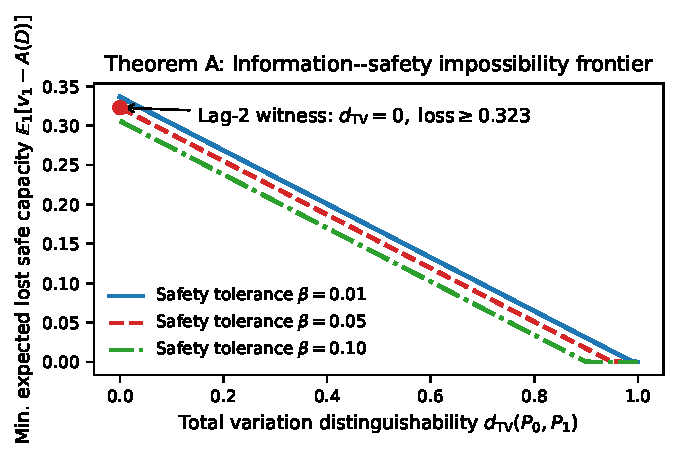
\includegraphics[width=0.48\textwidth]{figs/fig_flagship_2_tv_frontier.pdf}\hfill
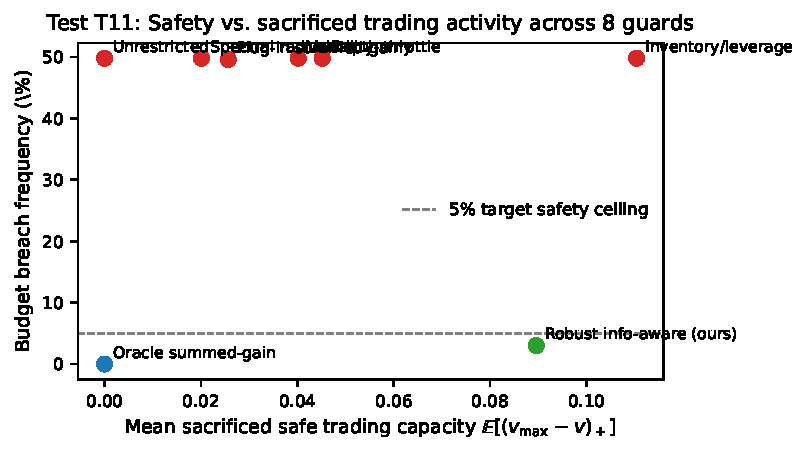
\includegraphics[width=0.48\textwidth]{figs/fig_flagship_5_guard_frontier.pdf}
\caption{Left: Information--safety impossibility frontier (Theorem~\ref{thm:flagship_A}, \texttt{T02}). Right: Safety breach rate versus sacrificed safe trading capacity across the eight risk-control methods of Table~\ref{tab:t11} (\texttt{T11}).}\label{fig:flagship25}
\end{figure}

Table~\ref{tab:t11} and Figure~\ref{fig:flagship25} summarize the experimental program (\texttt{T01}--\texttt{T12}). Across horizons $H=1,\ldots,8$, exhaustive sign enumeration over all $2^H$ disturbance sequences matches the cumulative convolution gain $G_{{\rm cum},H}$ to machine precision, while a peak-only repeated-trade gate breaches the unit risk budget by $71.5\%$ (\texttt{T05}). Under finite-sample calibration ($N=500$, \texttt{T04}), the $(1-\gamma)$ Mahalanobis region achieves $95.0\%$ empirical coverage and keeps false safety certifications at $0.0\%$ ($\le 5\%$ nominal). In the three-tier disclosure experiment (\texttt{T07}), moving from public lag-2 observations to class-tagged disclosure raises certified safe capacity from $0.178$ to $0.495$ (net welfare $+\$26.2$ after compliance and leakage costs), whereas in a low-heterogeneity high-compliance-cost regime net disclosure value is $-\$6.0$, confirming Theorem~\ref{thm:flagship_F}.
\section{Evidence from Binance futures depth}\label{sec:depth}

\subsection{Data and validation}
We use Binance USD-M BTCUSDT perpetual futures from the public archive: one-minute klines with taker-buy volume, \texttt{bookDepth} snapshots of cumulative depth within $\pm1$--$5\%$ of the mid at about 30-second intervals, and open interest from \texttt{metrics}. Depth is available from January 2023. No liquidation archive is available for this period, so we do not test liquidations.

Validation rules were fixed before analysis. A snapshot is kept if (V1) all of the $\pm1,2,5\%$ bands are present, (V2) depth is monotone in distance on each side, (V3) the implied average price at $\pm1\%$ is within 3\% of the one-minute close, and (V4) it is not part of a run of more than ten identical snapshots; (V5) a day is kept if at least 80\% of its minutes have a valid snapshot.

\begin{table}[t]\centering\small
\begin{threeparttable}
\caption{Depth data validation}\label{tab:d2}
\begin{tabular}{lr}
\toprule
Days requested (January 2023 -- October 2026) & 1{,}386\\
Days passing validation & 1{,}329\\
Snapshots examined & 3{,}897{,}951\\
\quad dropped by V1 (missing bands) & 0\\
\quad dropped by V2 (non-monotone) & 0\\
\quad dropped by V3 (implied price off by $>3\%$) & 98{,}080\\
\quad dropped by V4 (stuck feed) & 95{,}954\\
Failed periods & April 16 -- May 19, 2025; October 10--15, 2025\\
Training days used (2023--2024) & 718\\
\bottomrule
\end{tabular}
\begin{tablenotes}\footnotesize\item All files verified against published SHA-256 checksums. The 2025 failures coincide with archived depth that is misaligned with prices; the October 10, 2025 crash day is therefore unusable. \end{tablenotes}
\end{threeparttable}
\end{table}

\subsection{Structural estimates}
On one-minute bars, $p_t$ is the log price in basis points, $u_t$ signed taker flow in million USDT, $d_t=(B_1-A_1)/(B_1+A_1)$ the depth imbalance within 1\% of the mid, and $x_t=p_t-{\rm EMA}_{60}(p_t)$. Day by day we estimate
\begin{align*}
\Delta p_t&=\kappa u_t+\varphi d_{t-1}-(1-a)x_{t-1}+e_t,\\
d_t&=(1-r)d_{t-1}+\varepsilon u_t+e_t,\\
u_t&=(1-\eta)u_{t-1}+\eta q\,x_{t-1}+e_t,
\end{align*}
and form $\hat C_2$, $\hat C_3$ and the implied peak ratio $\max_k\hat h_k/\hat h_0$. The price equation has $\Delta p_t$ on the left, so the EMA filter does not create mechanical persistence. These are reduced-form regressions (flow is contemporaneous), so the estimates describe conditional dynamics rather than causal parameters.

\begin{table}[t]\centering
\begin{threeparttable}
\caption{Day-by-day T6 estimates, Binance BTCUSDT futures, training days 2023--2024}\label{tab:d3}
\small\setlength{\tabcolsep}{4pt}
\begin{tabular}{lccc}
\toprule
Median & All days & Top-decile volatility days & Other days\\
\midrule
$\hat\kappa$ (bp per \$1M) & 0.729 & 0.890 & 0.712\\
$\hat\varphi$ & $-0.051$ & 2.586 & $-0.138$\\
$\hat a$ & 0.970 & 0.980 & 0.969\\
$\hat r$ & 0.059 & 0.122 & 0.056\\
$\hat\varepsilon$ & $-0.0018$ & $-0.0017$ & $-0.0018$\\
$\hat\eta$ & 0.878 & 0.863 & 0.880\\
$\hat q$ & 0.018 & 0.012 & 0.019\\
$\hat C_3$ & $-0.0137$ & $-0.0111$ & $-0.0143$\\
\midrule
Mean $\hat C_3$ & $-0.0165$ & $-0.0167$ & $-0.0165$\\
\quad 95\% CI & [$-0.0176$, $-0.0155$] & [$-0.0219$, $-0.0122$] & [$-0.0175$, $-0.0154$]\\
Share of days $\hat C_3>0$ & 6.5\% & 5.6\% & 6.7\%\\
Share of days $\hat C_2>0$ & 0.8\% & 1.4\% & 0.8\%\\
Median peak ratio & 1.00 & 1.00 & 1.00\\
Days & 718 & 72 & 646\\
\bottomrule
\end{tabular}
\begin{tablenotes}\footnotesize\item One-minute bars. CIs from a day bootstrap. \end{tablenotes}
\end{threeparttable}
\end{table}

Table~\ref{tab:d3} has three findings. First, the market sits on the stable side of the condition: $\hat C_3<0$ on 93.5\% of days, and the median implied response peaks at impact. Second, the depletion coefficient $\hat\varepsilon$ is small and negative: taker buying is followed by slightly more ask-side than bid-side depth within 1\%, so in these re-centred bands the book appears to replenish rather than deplete the side being hit; Section~\ref{sec:fixedgrid} shows that a fixed price grid reverses the sign. With $\hat\varepsilon<0$, $\varphi\varepsilon$ is positive only if $\varphi$ is negative, which it is not on high-volatility days. Third, on high-volatility days depth imbalance moves prices strongly ($\hat\varphi=2.59$) and refill is twice as fast; the depth channel is active, but it works against amplification. The momentum term $\kappa^2\eta q$ is small (about $0.008$ at the medians), far below $(1-a)\kappa\approx0.022$.

\subsection{Does depth carry an overshoot?}
We estimate local projections \citep{jorda2005} of the cumulative price change on flow, $p_{t+k}-p_{t-1}=\beta_ku_t+\text{controls}$, with five lags of returns, flow and depth: (A) total; (B) adding cumulative future flow, which removes order-splitting persistence; and (C) adding cumulative future depth imbalance, which removes the depth channel. Theorem~\ref{thm:t6} predicts an overshoot ($\max_{k\ge1}\beta_k-\beta_0>0$) in (B) that shrinks in (C).

\begin{figure}[t]\centering
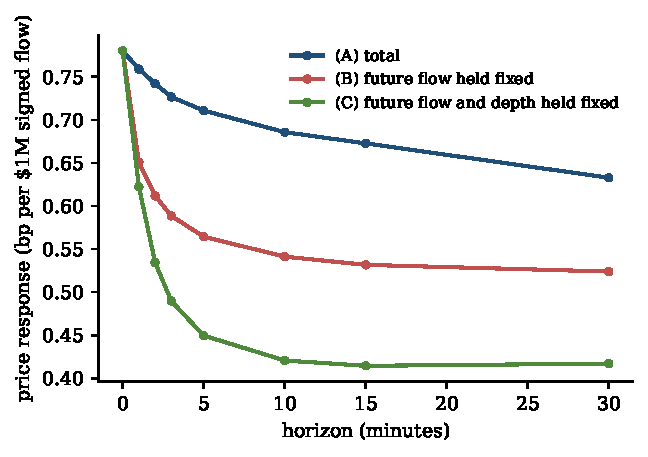
\includegraphics[width=0.6\textwidth]{figs/fig_mediation.pdf}
\caption{Price response to a \$1M flow shock, local projections on 716 training days. (A) total; (B) future flow held fixed; (C) future flow and depth held fixed.}\label{fig:med}
\end{figure}

\begin{table}[t]\centering\small
\begin{threeparttable}
\caption{Local-projection coefficients (bp per \$1M) and overshoots}\label{tab:d4}
\setlength{\tabcolsep}{3.5pt}
\begin{tabular}{lccccccccc}
\toprule
Minutes & 0 & 1 & 2 & 3 & 5 & 10 & 15 & 30 & Overshoot\\
\midrule
(A) total & 0.780 & 0.759 & 0.742 & 0.727 & 0.711 & 0.686 & 0.673 & 0.633 & $-0.021$\\
 & & & & & & & & & [$-0.027$, $-0.015$]\\
(B) flow fixed & 0.780 & 0.651 & 0.612 & 0.589 & 0.564 & 0.541 & 0.532 & 0.524 & $-0.129$\\
 & & & & & & & & & [$-0.134$, $-0.124$]\\
(C) flow, depth fixed & 0.780 & 0.622 & 0.534 & 0.490 & 0.450 & 0.421 & 0.414 & 0.417 & $-0.158$\\
 & & & & & & & & & [$-0.164$, $-0.152$]\\
\bottomrule
\end{tabular}
\begin{tablenotes}\footnotesize\item 716 training days; day bootstrap. \end{tablenotes}
\end{threeparttable}
\end{table}

There is no overshoot (Figure~\ref{fig:med}, Table~\ref{tab:d4}). The overshoot statistic is negative in every version. Holding depth fixed makes the response decay faster, consistent with depth that partly sustains the price move but never pushes it past impact.

\subsection{Pre-registered out-of-sample test}
Before opening the test period we registered the specification (SHA-256 \texttt{d95212187ae4\ldots}): hourly blocks (06:00--23:00 UTC); $\hat C_3$ estimated from the previous six hours and winsorized at training percentiles; outcome the next hour's maximum adverse excursion (MAE, bp); controls for realized volatility (1 and 6 hours), absolute return, flow imbalance, volume, depth, imbalance and open-interest change; OLS on 2023--2024 and evaluation on 2025--2026. Success required a one-sided Clark--West $p<0.05$ \emph{and} a day-block bootstrap 95\% CI for $\Delta R^2$ excluding zero. Secondary candidates and outcomes are Holm-adjusted. The test set was opened once. An audit that scrambles all data from $t$ onward left every feature unchanged in 30 of 30 trials.

\begin{table}[t]\centering
\begin{threeparttable}
\caption{Out-of-sample test, 2025--2026 (train 12,896 hours, test 10,979 hours)}\label{tab:d8}
\small\setlength{\tabcolsep}{4pt}
\begin{tabular}{llccc}
\toprule
Outcome & Candidate & $\Delta R^2$ (pts) [95\% CI] & $\Delta$AUC [95\% CI] & Holm $p$\\
\midrule
MAE (primary) & $\hat C_3$ & $+0.018$ [$-0.100$, $+0.132$] & $+0.0001$ [$-0.0009$, $+0.0012$] & ---\\
MAE & peak ratio & $+0.010$ [$+0.001$, $+0.019$] & $+0.0001$ [$-0.0000$, $+0.0002$] & 0.032\\
OI drop & $\hat C_3$ & $-0.045$ [$-0.095$, $-0.003$] & $-0.0049$ [$-0.0083$, $-0.0016$] & 0.787\\
OI drop & peak ratio & $+0.102$ [$+0.061$, $+0.231$] & $-0.0014$ [$-0.0067$, $+0.0037$] & $<0.001$\\
Depth collapse & $\hat C_3$ & $+0.181$ [$-0.156$, $+0.484$] & $+0.0071$ [$+0.0041$, $+0.0105$] & $<0.001$\\
Depth collapse & peak ratio & $+0.159$ [$+0.094$, $+0.234$] & $+0.0009$ [$+0.0004$, $+0.0014$] & $<0.001$\\
\bottomrule
\end{tabular}
\begin{tablenotes}\footnotesize\item Primary: Clark--West one-sided $p=0.023$, but the $\Delta R^2$ CI contains zero, so the pre-registered test fails. Baseline $R^2$ for MAE is 0.293; baseline AUC 0.812. \end{tablenotes}
\end{threeparttable}
\end{table}

The primary test fails (Table~\ref{tab:d8}): $\hat C_3$ adds $0.018$ percentage points of out-of-sample $R^2$ with a confidence interval that includes zero. Some secondary effects are statistically significant after Holm correction, notably for depth collapse, but they are economically negligible: no candidate adds more than $0.2$ points of $R^2$ or $0.01$ of AUC.

\paragraph{A volatility flag does better.} We set two flags on training data, each to flag 10\% of hours: high $\hat C_3$ and high realized volatility. On the 909 tail hours of the test period (MAE above the training 90th percentile), the $\hat C_3$ flag has precision $8.6\%$ and recall $19.5\%$; the volatility flag has precision $38.1\%$ and recall $37.1\%$; the union has precision $16.3\%$ and recall $49.4\%$. The unconditional tail rate is about 10\%, so the $\hat C_3$ flag is no better than chance.

\subsection{Crash events}
For each event day we compute $\hat C_3$ hour by hour and its percentile in the training distribution during the three hours before the worst hour (Figure~\ref{fig:events}, Table~\ref{tab:d9}). $\hat C_3$ was elevated before these events but stayed negative throughout, and three events are not a test.

\begin{table}[t]\centering\small
\begin{threeparttable}
\caption{Event days}\label{tab:d9}
\begin{tabular}{lcccc}
\toprule
Event & Worst hour & Worst MAE & $\hat C_3$ percentile, & OI change\\
 & (UTC) & (bp) & 3 hours before & in worst hour\\
\midrule
SVB, 2023-03-11 & 7 & 214.8 & 82 & $+2.5\%$\\
Yen carry unwind, 2024-08-05 & 13 & 724.0 & 93, 84, 83 & $-0.8\%$\\
Tariff shock, 2025-04-07 & 14 & 357.8 & 97, 98, 38 & $+3.1\%$\\
2025-10-10 & \multicolumn{4}{c}{no valid depth data}\\
\bottomrule
\end{tabular}
\begin{tablenotes}\footnotesize\item SVB has one valid hour before its worst hour. \end{tablenotes}
\end{threeparttable}
\end{table}

\begin{figure}[t]\centering
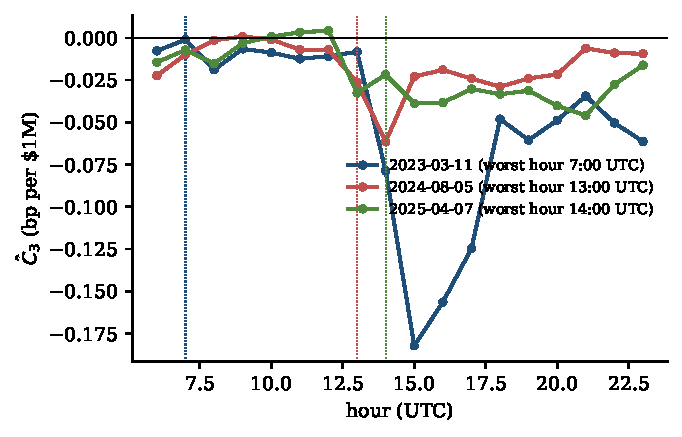
\includegraphics[width=0.6\textwidth]{figs/fig_events.pdf}
\caption{Hourly $\hat C_3$ on three event days (UTC). Values stay below zero, the amplification threshold.}\label{fig:events}
\end{figure}

\section{Evidence from spot prices}\label{sec:spot}

\subsection{A unit-free amplification statistic}
The earlier version measured amplification by the norm of powers of a VAR(1) operator on (price deviation, flow), estimated over ten-minute windows of one-second Binance spot data. That norm depends on the units of the state: multiplying prices by 10 and dividing flow by 1,000 changed the raw norm from $8.73$ to $86{,}731$ on the same window. Proposition~\ref{prop:invariance} explains why: state norms are not invariant to coordinates. We therefore standardize the state, $\tilde J=D^{-1}\hat JD$ with $D={\rm diag}({\rm sd}\,x,{\rm sd}\,f)$, and use $M_{\rm std}=\max_k\|e_x^\top\tilde J^k\|$, which is invariant to units (verified). We also report the price-to-price amplification $A_{xx}=\max_k|(\hat J^k)_{11}|$ and a delayed-peak statistic ${\rm hump}=\max_k|(\hat J^k)_{12}|/|\hat J_{12}|$.

\subsection{Crash days and a no-feedback null}
We study five crash days: May 19, 2021; LUNA, May 9, 2022; FTX, November 8, 2022; SVB, March 11, 2023; and August 5, 2024. Windows are selected \emph{ex ante} (previous ten minutes in the top volatility decile), and for comparison by outcome (the ten largest absolute returns). A no-feedback null keeps each window's real flow, generates prices with no feedback, $\Delta p=\hat\kappa f+\hat\sigma e$, and pushes them through the identical pipeline.

\begin{table}[t]\centering\small
\begin{threeparttable}
\caption{Unit-free amplification on crash days and the no-feedback null}\label{tab:spotnull}
\begin{tabular}{lccccc}
\toprule
Event & Windows (ex ante) & Mean $M_{\rm std}$ & Null 99th pct & $p$ (vs null) & Outcome-selected mean\\
\midrule
May 2021 & 142 & 1.0000 & 1.00002 & 1.00 & 1.0000\\
LUNA 2022 & 57 & 1.00008 & 1.00006 & 0.039 & 1.00045\\
FTX 2022 & 49 & 1.0000 & 1.00029 & 1.00 & 1.0000\\
SVB 2023 & 6 & 1.00006 & 1.00025 & 0.059 & 1.00032\\
Aug 2024 & 108 & 1.0000 & 1.00007 & 1.00 & 1.0000\\
\bottomrule
\end{tabular}
\begin{tablenotes}\footnotesize\item Ten-minute windows of one-second bars. The median hump statistic is 1.000 in every event and its null $p$-value is 1.00. In the ordinary 2021--2023 panel, 0.2\% of windows have $A_{xx}>1$ and the 95th percentile of $M_{\rm std}$ is 1.0000; a handful of near-singular windows produce very large values, so ordinary-window means are not informative. \end{tablenotes}
\end{threeparttable}
\end{table}

Only LUNA exceeds the null, by less than $0.01\%$ (Table~\ref{tab:spotnull}). Outcome-selected windows give only marginally larger values ($\le1.0005$). Stress-window means exceed the ordinary 95th percentile in two events, by amounts of the same size. The pre-registered gate fails: unit-free transient amplification in spot data is indistinguishable from one and from the pipeline null. Varying the EMA span (60, 120, 300 seconds) and the bar length (1 or 5 seconds) does not change this; crash-day means range from $1.0003$ to $1.18$ across specifications and are never above the corresponding ordinary means.

\subsection{Overshoot with flow held fixed}
Local projections on one-second data give the price response to a \$1M flow shock (Table~\ref{tab:spotlp}). On ordinary days, with future flow held fixed, there is a small, short-lived overshoot of $+0.248$ [$0.133$, $0.376$] bp per \$1M, peaking at two seconds and decaying after. On crash days the flow-fixed overshoot is negative, $-0.277$ [$-0.528$, $-0.042$]. The large total overshoots ($+0.91$ ordinary, $+2.40$ crash) disappear when future flow is held fixed: they come from order splitting, not from the book.

\begin{table}[t]\centering\small
\begin{threeparttable}
\caption{Spot local projections (bp per \$1M)}\label{tab:spotlp}
\setlength{\tabcolsep}{3.5pt}
\begin{tabular}{lcccccccccc}
\toprule
Seconds & 0 & 1 & 2 & 5 & 10 & 20 & 30 & 60 & 120 & 300\\
\midrule
Ordinary, total & 5.86 & 6.28 & 6.53 & 6.60 & 6.69 & 6.77 & 6.67 & 6.49 & 6.39 & 5.92\\
Ordinary, flow fixed & 5.86 & 6.02 & 6.11 & 5.90 & 5.68 & 5.26 & 4.86 & 4.16 & 3.37 & 1.99\\
Crash, total & 6.69 & 6.85 & 6.92 & 7.13 & 7.75 & 8.20 & 8.46 & 8.20 & 9.09 & 8.96\\
Crash, flow fixed & 6.69 & 6.41 & 6.28 & 5.99 & 5.95 & 5.46 & 5.02 & 3.88 & 3.10 & $-0.08$\\
\bottomrule
\end{tabular}
\begin{tablenotes}\footnotesize\item\end{tablenotes}
\end{threeparttable}
\end{table}

\subsection{Pre-registered predictive test}
Before opening 2024, we registered (SHA-256 \texttt{b1fd7f8e\ldots}) a test of whether pre-window amplification predicts the next ten minutes' MAE beyond volatility and flow controls, on non-overlapping 30-minute blocks (train 2021--2023, 3,307 blocks; test 2024, 1,104 blocks). It does not: $\Delta R^2=-0.023$ points [$-0.056$, $-0.002$], Clark--West $p=0.966$, AUC $0.822$ in both models. A random feature with the same autocorrelation gives $\Delta R^2=-0.020$ points, the same as the candidate. Leave-one-year-out fits within the training period are unstable (the 2023 fold gives a very large negative $\Delta R^2$ because of outlying candidate values), so the null result does not depend on one year being unusual.

The test set was opened three times. The first evaluations stopped on a numerical error from degenerate windows; the fix drops blocks with non-finite features (five blocks) and is the only change, and the registered specification hash is unchanged. A volatility flag again dominates: precision $43\%$ and recall $30\%$ against $3\%$ and $10\%$ for the amplification flag; the difference in recall has a CI of $[-0.37,0.13]$.

\section{Evidence from thinner books}\label{sec:thin}

The deepest book in crypto is the least likely place to find amplification. This section moves to thinner books. It reports the pre-registered out-of-sample tests in thin Binance books, on Bybit and in thin US stocks, failures included, and labels every check decided after a test set was opened as post hoc. Figure~\ref{fig:forest} collects all out-of-sample evaluations of this section.

\subsection{Design}\label{sec:thin_design}
We fixed 30 Binance USD-M perpetuals from the quote-volume ranking of one training day (June 10, 2024) before computing any T6 statistic, spread from BTCUSDT to symbols with under \$5M daily volume. Data are sampled on the 10th and 24th of each month from January 2023 to September 2026 and pass the validation rules V1--V5 of Section~\ref{sec:depth}: 2{,}565 of 2{,}700 symbol-days are valid; of 7{,}486{,}444 snapshots, V3 drops 212{,}745 and V4 drops 161{,}280, and V1 and V2 drop none. Liquidity terciles are fixed on median training-period depth within 1\% of the mid. The thin tercile has \$0.22M--\$0.38M of depth within 1\%, the thick tercile \$0.97M--\$220M. Flow is divided by each symbol's median absolute one-minute training flow, so that $\hat\kappa$ is in basis points per typical minute of flow. All other definitions follow Section~\ref{sec:depth}. An audit that scrambles all data from $t$ onward left every hourly feature unchanged in 30 of 30 trials.

\subsection{The cross-section of the amplification condition}

\begin{table}[t]\centering
\begin{threeparttable}
\caption{T6 estimates by liquidity tercile, 30 USD-M perpetuals, training days 2023--2024}\label{tab:x3}
\small\setlength{\tabcolsep}{5pt}
\begin{tabular}{lccc}
\toprule
 & Thick & Mid & Thin\\
\midrule
Mean $\hat C_3$ & $-0.0297$ & $-0.0216$ & $-0.0324$\\
\quad 95\% CI & [$-0.0341$, $-0.0257$] & [$-0.0250$, $-0.0185$] & [$-0.0386$, $-0.0268$]\\
Share of symbol-days with $\hat C_3>0$ & 9.4\% & 15.2\% & 16.1\%\\
Median $\hat\varphi$ & 2.33 & 2.38 & 3.11\\
Median $\hat\varepsilon$ & $-0.0014$ & $-0.0006$ & $-0.0005$\\
Share with $\hat\varepsilon>0$ & 11.1\% & 24.4\% & 30.1\%\\
Mean feedback loop gain $\hat Q$ & 0.0091 & 0.0033 & 0.0016\\
\midrule
\multicolumn{4}{l}{Spearman correlation with log depth across the 30 symbols [95\% CI]}\\
\quad mean $\hat C_3$ & \multicolumn{3}{c}{$-0.001$ [$-0.37$, $0.38$]}\\
\quad share $\hat C_3>0$ & \multicolumn{3}{c}{$-0.59$ [$-0.81$, $-0.27$]}\\
\quad $\hat Q$ & \multicolumn{3}{c}{$+0.70$ [$0.41$, $0.87$]}\\
\bottomrule
\end{tabular}
\begin{tablenotes}\footnotesize\item 1{,}424 training symbol-days, ten symbols per tercile. CIs from a symbol-day bootstrap (tercile rows) and a symbol bootstrap (correlations). $\hat Q$ is the loop gain of the companion paper estimated on one-minute bars; a placebo random walk with each day's volatility gives $\hat Q\approx0$ for every symbol. \end{tablenotes}
\end{threeparttable}
\end{table}

Table~\ref{tab:x3} confirms the BTCUSDT result across liquidity: mean $\hat C_3$ is negative in every tercile, and taker flow on average does not deplete the side it hits ($\hat\varepsilon<0$ at the median everywhere). What changes with depth is the frequency of the amplifying regime, not its average. The share of symbol-days with $\hat C_3>0$ rises from 9.4\% in the thick tercile to 16.1\% in the thin tercile, with a Spearman correlation of $-0.59$ against log depth. Depth sensitivity $\hat\varphi$ is larger, and depletion is less negative and more often positive, in thinner books. We had predicted a negative correlation between log depth and mean $\hat C_3$; that prediction fails ($\rho=-0.001$).

The last row is an unexpected finding for the companion paper. Measured feedback $\hat Q$ is larger in \emph{deeper} books ($\rho=+0.70$): flow responds to price deviations most where liquidity, and plausibly algorithmic participation, is greatest. Feedback and amplification are therefore different objects. Deep books have more feedback and refill fast enough to absorb it; thin books have less feedback and, more often, too little reversion.

\subsection{Overshoot and depletion}

\begin{table}[t]\centering\small
\begin{threeparttable}
\caption{Local-projection overshoot by tercile, $\max_{k\ge1}\beta_k-\beta_0$ [95\% CI]}\label{tab:x4}
\setlength{\tabcolsep}{3pt}
\begin{tabular}{lccc}
\toprule
 & Thick & Mid & Thin\\
\midrule
(A) total & $-0.045$ [$-0.079$, $0.047$] & $-0.034$ [$-0.054$, $0.024$] & $+0.007$ [$-0.050$, $0.083$]\\
(B) future flow fixed & $-0.181$ [$-0.211$, $-0.152$] & $-0.075$ [$-0.091$, $-0.058$] & $-0.073$ [$-0.094$, $-0.051$]\\
(C) flow and depth fixed & $-0.243$ [$-0.276$, $-0.212$] & $-0.121$ [$-0.140$, $-0.102$] & $-0.113$ [$-0.135$, $-0.092$]\\
Symbol-days & 459 & 460 & 445\\
\bottomrule
\end{tabular}
\begin{tablenotes}\footnotesize\item Basis points per typical minute of flow, horizons 0--30 minutes; local projections are estimated per symbol-day and averaged, with a symbol-day bootstrap. \end{tablenotes}
\end{threeparttable}
\end{table}

With future flow held fixed there is no overshoot in any tercile (Table~\ref{tab:x4}); the registered prediction of a positive (B) overshoot in thin books fails. The response decays less in thin than in thick books, and holding depth fixed again makes it decay faster, as in Table~\ref{tab:d4}.

To check that replenishment is not an artefact of one-minute aggregation, we sum signed taker flow exactly between consecutive depth snapshots from trade-level data and estimate depletion $\varepsilon_{30}$ at about 30 seconds, with an additional coefficient on sweeps (intervals in the top decile of absolute flow). Table~\ref{tab:x8} reports five symbols on six training days each.

\begin{table}[t]\centering\small
\begin{threeparttable}
\caption{Depletion at the snapshot scale (about 30 seconds)}\label{tab:x8}
\setlength{\tabcolsep}{2.5pt}
\begin{tabular}{llcccc}
\toprule
Symbol & Tercile & $\hat\varepsilon_{30}$ [95\% CI] & Sweep extra [95\% CI] & $\hat\varepsilon$, 1 minute & Days $\hat\varepsilon_{30}>0$\\
\midrule
BTCUSDT & thick & $-0.0045$ [$-0.0058$, $-0.0033$] & $+0.0034$ [$0.0023$, $0.0046$] & $-0.0025$ & 0 of 6\\
XMRUSDT & mid & $-0.0042$ [$-0.0058$, $-0.0029$] & $+0.0037$ [$0.0025$, $0.0051$] & $-0.0011$ & 0 of 6\\
RLCUSDT & thin & $-0.0034$ [$-0.0065$, $-0.0012$] & $+0.0029$ [$0.0011$, $0.0058$] & $-0.0003$ & 1 of 6\\
CELRUSDT & thin & $-0.0015$ [$-0.0032$, $0.0001$] & $+0.0017$ [$0.0004$, $0.0031$] & $-0.0004$ & 2 of 6\\
CVXUSDT & thin & $+0.0010$ [$-0.0033$, $0.0060$] & $-0.0003$ [$-0.0040$, $0.0027$] & $+0.0004$ & 2 of 6\\
\bottomrule
\end{tabular}
\begin{tablenotes}\footnotesize\item Day bootstrap over six training days per symbol. Depth is measured in bands of $\pm1\%$ around the current mid, so a price move also recenters the band; this biases $\hat\varepsilon_{30}$ in an unknown direction. \end{tablenotes}
\end{threeparttable}
\end{table}

In these re-centred bands, replenishment is stronger, not weaker, at 30 seconds: $\hat\varepsilon_{30}$ is negative with a CI below zero in three of five symbols and is never significantly positive. Sweeps offset most of it, so a sweep leaves the hit side about as deep as before ($\hat\varepsilon_{30}$ plus the sweep coefficient lies between $-0.0012$ and $+0.0007$). On this measure, the depletion channel that drives Theorem~\ref{thm:t6} would be absent even in thin books; the next subsection shows that the measure itself is biased toward replenishment.

\subsection{Depletion on a fixed price grid}\label{sec:fixedgrid}
Binance's depth archive reports depth within bands around the \emph{current} mid. After a buy moves the mid up, the ask band shifts into deeper resting orders and the bid band away from resting bids, which mechanically makes the book look ask-heavy after a buy, the sign we estimate. Bybit's order-book files contain every level, so the band can be held fixed at the previous mid. After seeing Table~\ref{tab:x8} we computed, for the six coins of Table~\ref{tab:bybitob} on four days each, the change in depth imbalance over 30-second intervals regressed on signed taker flow, once with the band fixed at the start-of-interval mid and once re-centred at the end-of-interval mid, Binance's construction.

\begin{table}[t]\centering\small
\begin{threeparttable}
\caption{Depletion at 30 seconds with a fixed and a re-centred band (Bybit order books, post hoc)}\label{tab:fixedgrid}
\begin{tabular}{lccc}
\toprule
Band & $\hat\varepsilon_{30}$ [95\% CI] & Share $>0$ & Coin-days\\
\midrule
Fixed at previous mid & $+0.0021$ [$+0.0013$, $+0.0032$] & 95\% & 20\\
Re-centred (Binance) & $-0.0004$ [$-0.0007$, $-0.0001$] & 30\% & 20\\
\bottomrule
\end{tabular}
\begin{tablenotes}\footnotesize\item ACH, ALICE, API3, LIT, WOO and ZEN, May 11--12 and September 11--12, 2025; flow normalized by each coin-day's median absolute 30-second flow; mean over coin-days with a bootstrap interval. Post hoc. Kind: real data (Part 13, \texttt{R5}).\end{tablenotes}
\end{threeparttable}
\end{table}

The sign reverses (Table~\ref{tab:fixedgrid}). With the band fixed, buying depletes the ask side in 19 of 20 coin-days; with the band re-centred, the same data reproduce the replenishment of Tables~\ref{tab:d3} and~\ref{tab:x8}. The replenishment finding is therefore an artefact of band recentring, and depletion is present. Two conclusions survive. First, local projections show no peak overshoot once future flow is held fixed (Table~\ref{tab:x4}), so depletion is not large enough to satisfy $\varphi\varepsilon>(1-a)\kappa$ in the data we observe; second, the depth term carries no out-of-sample forecasting content (Tables~\ref{tab:y6} and~\ref{tab:z6}). Both statements rest on Binance's re-centred depth measure, and a fixed-grid measure of $\varphi\varepsilon$ in the same books would require order-level Binance data that are not public.

\subsection{Pre-registered test in thin books}\label{sec:x6}
Before opening 2025--2026 for these symbols we registered the specification (SHA-256 \texttt{5910b6b4d90a\ldots}). It is identical to Section~\ref{sec:depth} except for three changes, all fixed in advance: the primary sample is the thin tercile; the regressions include symbol fixed effects; and the bootstrap resamples dates, with all symbols on a date kept together. The test cell was executed twice in the same session. The specification hash, the code and the data were unchanged between the two runs, and the evaluation is deterministic, so both runs give the numbers below; we report the count because the protocol requires it.

\begin{table}[t]\centering
\begin{threeparttable}
\caption{Pre-registered test, 30 symbols, 2025--2026}\label{tab:x6}
\small\setlength{\tabcolsep}{4pt}
\begin{tabular}{llccc}
\toprule
Sample & Outcome $\mid$ candidate & $\Delta R^2$ (pts) [95\% CI] & $\Delta$AUC [95\% CI] & Holm $p$\\
\midrule
Thin (primary) & MAE $\mid\hat C_3$ & $+1.216$ [$+0.273$, $+7.987$] & $+0.012$ [$+0.003$, $+0.019$] & ---\\
Thin & MAE $\mid$ peak ratio & $+0.065$ [$-0.072$, $+0.108$] & $+0.000$ [$-0.000$, $+0.001$] & 0.207\\
Thin & depth collapse $\mid\hat C_3$ & $-2.111$ [$-3.127$, $-1.173$] & $-0.012$ [$-0.023$, $-0.003$] & 1.000\\
Thin & OI drop $\mid\hat C_3$ & $+0.184$ [$-0.242$, $+1.128$] & $+0.040$ [$+0.017$, $+0.061$] & $<0.001$\\
Mid & MAE $\mid\hat C_3$ & $+0.003$ [$-0.056$, $+0.875$] & $+0.002$ [$-0.002$, $+0.005$] & 0.551\\
Thick & MAE $\mid\hat C_3$ & $+0.039$ [$-0.244$, $+0.057$] & $-0.001$ [$-0.003$, $+0.000$] & 0.361\\
All 30 & MAE $\mid\hat C_3$ & $+0.117$ [$-0.015$, $+1.736$] & $+0.003$ [$-0.000$, $+0.006$] & $<0.001$\\
\bottomrule
\end{tabular}
\begin{tablenotes}\footnotesize\item Primary: train 8{,}340 and test 6{,}521 symbol-hours on ten symbols; Clark--West $t=8.53$, one-sided $p<0.001$; baseline out-of-sample $R^2=0.025$; AUC $0.768\to0.780$. The pre-registered test passes. Holm $p$ is the Clark--West $p$-value adjusted across the six secondary tests. Date-block bootstrap with 2{,}000 draws; bootstrap CIs are right-skewed because a few volatile dates carry much of the variation. \end{tablenotes}
\end{threeparttable}
\end{table}

The primary test passes (Table~\ref{tab:x6}). In thin books, $\hat C_3$ estimated from the previous six hours adds $1.2$ points of out-of-sample $R^2$ for the next hour's maximum adverse excursion, beyond realized volatility, flow, volume, depth, imbalance and open interest, and raises the AUC for tail hours by $0.012$. The effect is confined to thin books: in the mid and thick terciles it is zero, and in the pooled sample the Clark--West test rejects but the $\Delta R^2$ interval contains zero. $\hat C_3$ also helps classify hours with a large open-interest drop, but it predicts depth collapse \emph{worse} than the baseline, again pointing away from the depth channel.

\paragraph{Flags.} On training data we set a $\hat C_3$ flag and a volatility flag; 575 of 6{,}521 test hours (8.8\%) are tail hours. The $\hat C_3$ flag fires in 8.9\% of hours with precision 16.5\% and recall 16.7\%, about twice the base rate. The volatility flag, which fires more often (16.0\%), does better (precision 23.4\%, recall 42.4\%), and the union reaches recall 51.1\% at precision 19.5\%. $\hat C_3$ is a useful addition to volatility in thin books, not a replacement for it.

\subsection{Tick size: a caution and a robustness check}\label{sec:tick}

\paragraph{Tick changes.} We located tick changes by inferring each day's price grid and dating changes by binary search over daily files. We found 12 tick reductions, all by a factor of ten, on 11 symbols (GMTUSDT twice) between August 2023 and August 2026; nine fall in the test period. A difference-in-differences design compares 10 days before and after each event with four control symbols of similar liquidity. After a tick cut, $\hat C_3$ rises with a CI above zero in 10 of 12 events, but realized volatility in basis points falls sharply at the same time (by up to 32 bp on ALICEUSDT), and the implied peak ratio does not change in any event (every CI includes zero). The Spearman correlation between the change in refill $\hat r$ and the change in the peak ratio is $-0.04$. We read this as a measurement result, not a test of the theory: at a coarse tick, prices move in discrete steps and the basis-point scale of $\hat C_3$ changes mechanically when the grid changes. The natural experiment cannot test the prediction that faster refill lowers the overshoot.

\paragraph{Does tick size drive Table~\ref{tab:x6}?} Eleven of the 30 symbols, six of them thin, changed tick, and five of those six did so inside the test period. After seeing Table~\ref{tab:x6} we therefore ran the post-hoc checks of Table~\ref{tab:x6r}, counted separately (one evaluation).

\begin{table}[t]\centering\small
\begin{threeparttable}
\caption{Post-hoc tick-size robustness of the thin-book result}\label{tab:x6r}
\setlength{\tabcolsep}{3pt}
\begin{tabular}{p{0.34\textwidth}cccc}
\toprule
Check & Symbols & Test hours & $\Delta R^2$ (pts) [95\% CI] & Clark--West $p$\\
\midrule
R0 baseline (Table~\ref{tab:x6}) & 10 & 6{,}521 & $+1.216$ [$+0.295$, $+8.017$] & $<0.001$\\
R1 + relative tick size and its log & 10 & 6{,}485 & $+1.243$ [$+0.373$, $+7.627$] & $<0.001$\\
R2 drop symbols with any tick change & 4 & 2{,}639 & $+0.511$ [$-0.069$, $+2.061$] & $<0.001$\\
R3 only days with the training tick & 10 & 5{,}642 & $+1.131$ [$+0.256$, $+9.305$] & $<0.001$\\
R1 and R3 together & 10 & 5{,}642 & $+1.222$ [$+0.357$, $+9.410$] & $<0.001$\\
R4 outcome in ticks & 10 & 6{,}485 & $-0.127$ [$-0.319$, $-0.018$] & 0.991\\
R5 $\hat C_3$ percentile within symbol & 10 & 6{,}521 & $+0.158$ [$-0.013$, $+1.322$] & 0.026\\
R6 leave one symbol out (10 fits) & 9 & & $+0.698$ to $+1.760$, all CIs $>0$ & all $<0.001$\\
\bottomrule
\end{tabular}
\begin{tablenotes}\footnotesize\item Post hoc: decided after Table~\ref{tab:x6}. 500 date-block bootstrap draws (200 in R6). \end{tablenotes}
\end{threeparttable}
\end{table}

The result survives controls for tick size, the removal of every day traded at a tick different from training, and the removal of any single symbol (Table~\ref{tab:x6r}). It weakens when the six thin symbols that ever changed tick are dropped: four remain, and the point estimate halves with an interval that just includes zero. It disappears when the outcome is measured in ticks; at each tick cut this outcome jumps tenfold, a break the training fit cannot anticipate, so we regard R4 as a weak test, but we report it. A scale-free version of the candidate (its percentile within each symbol's training distribution) is weak. Our reading is that $\hat C_3$'s forecasting content is tied to its \emph{level}, which mixes the amplification balance with the basis-point scale of each book. Sections~\ref{sec:y6} and~\ref{sec:y8} test whether that level is more than a measure of scale.

\subsection{Out-of-sample replication on new symbols}\label{sec:y6}
A result found in ten symbols could be specific to them. We therefore drew 24 new symbols, seeded and before any analysis, from the 72 USD-M perpetuals that were not in the original 30 and whose training-day volume was at most 1.5 times that of the most liquid thin symbol. We applied the same validation (2{,}090 of 2{,}160 symbol-days valid) and classified symbols as thin with a cut fixed in advance at the boundary between the original thin and mid terciles (\$0.39M of depth within 1\%). Ten new symbols are thin (ACH, ARPA, CHR, GTC, HOT, IOTX, OGN, SPELL, T and ZEN, all USDT-margined) and 14 are not. A new specification (SHA-256 \texttt{6aa8e2c03d79\ldots}) fixed the primary test identical to Table~\ref{tab:x6} and, as secondary tests, the three terms of $C_3$ separately, a unit-free ratio $A=(\varphi\varepsilon+\kappa^2\eta q)/((1-a)\kappa)-1$ that is positive exactly when $C_3>0$, and the not-thin group. The test set was opened once.

\begin{table}[t]\centering
\begin{threeparttable}
\caption{Pre-registered replication on ten new thin symbols, 2025--2026}\label{tab:y6}
\small\setlength{\tabcolsep}{4pt}
\begin{tabular}{llccc}
\toprule
Sample & Candidate & $\Delta R^2$ (pts) [95\% CI] & $\Delta$AUC [95\% CI] & Holm $p$\\
\midrule
Thin (primary) & $\hat C_3$ & $+0.845$ [$+0.303$, $+6.371$] & $+0.008$ [$+0.002$, $+0.013$] & ---\\
Thin & momentum term $\kappa^2\eta q$ & $+0.641$ [$+0.395$, $+3.242$] & $+0.003$ [$-0.001$, $+0.008$] & $<0.001$\\
Thin & reversion term $(1-a)\kappa$ & $+0.688$ [$+0.204$, $+5.606$] & $+0.008$ [$+0.003$, $+0.012$] & $<0.001$\\
Thin & depth term $\varphi\varepsilon$ & $+0.013$ [$-0.213$, $+1.155$] & $-0.001$ [$-0.005$, $+0.003$] & 0.308\\
Thin & unit-free ratio $A$ & $-0.045$ [$-0.096$, $-0.031$] & $-0.000$ [$-0.001$, $+0.000$] & 0.974\\
Not thin (14) & $\hat C_3$ & $-0.042$ [$-0.131$, $+0.780$] & $+0.002$ [$-0.003$, $+0.007$] & 0.308\\
\bottomrule
\end{tabular}
\begin{tablenotes}\footnotesize\item Primary: train 8{,}520 and test 7{,}092 symbol-hours; Clark--West $t=11.66$, one-sided $p<0.001$; AUC $0.768\to0.776$; training coefficient $+54.3$ (Table~\ref{tab:x6}: $+88.3$). Training coefficients: momentum $+104.3$, reversion $-53.0$. The pre-registered replication passes. \end{tablenotes}
\end{threeparttable}
\end{table}

The result replicates (Table~\ref{tab:y6}). On symbols never used before, $\hat C_3$ adds $0.85$ points of out-of-sample $R^2$ with an interval excluding zero, and improves tail classification. It again has no value outside thin books. The decomposition shows where the forecasting content lies, and every sign matches Theorem~\ref{thm:t6} and Proposition~\ref{prop:t6m}. A larger momentum term predicts larger adverse excursions; a larger reversion term, which pushes $C_3$ down, predicts smaller ones; and the depth term, whose depletion factor is close to zero (Table~\ref{tab:x8}), predicts nothing. In training data the reversion term is by far the largest component (median $0.033$, against $-0.0009$ for momentum and $-0.0003$ for depth), so most of the variation in $\hat C_3$ is variation in impact-weighted mean reversion.

The unit-free ratio fails. Because the amplifying terms are small, its median is $-0.996$ and its variation is mostly the noise of a ratio with an estimated denominator. Together with R5 in Table~\ref{tab:x6r}, this means that on these samples the forecasting content was tied to the level of $\hat C_3$. Section~\ref{sec:z6} tests two better-behaved unit-free statistics on fresh data.

\subsection{Is $\hat C_3$ just price impact?}\label{sec:y8}
Both working terms contain the impact coefficient $\kappa$, so $\hat C_3$ might forecast excursions only because it measures illiquidity. After seeing Table~\ref{tab:y6} we added four impact controls, all from the same past six hours or hour and winsorized at training percentiles: $\hat\kappa$ from the same fit, $\hat\kappa^2$, a univariate Kyle's $\lambda$ \citep{kyle1985} (slope of returns on signed flow) and a log Amihud ratio \citep{amihud2002} (absolute return over volume). This is a post-hoc check, evaluated once and counted separately.

\begin{table}[t]\centering\small
\begin{threeparttable}
\caption{Post-hoc price-impact controls, ten new thin symbols, 2025--2026}\label{tab:y8}
\begin{tabular}{lccc}
\toprule
Candidate $\mid$ added controls & $\Delta R^2$ (pts) [95\% CI] & $\Delta$AUC [95\% CI] & Clark--West $t$\\
\midrule
$\hat C_3$ $\mid$ none (Table~\ref{tab:y6}) & $+0.845$ [$+0.303$, $+6.371$] & $+0.008$ [$+0.002$, $+0.013$] & 11.66\\
$\hat C_3$ $\mid$ $\hat\kappa$, $\hat\kappa^2$ & $+0.755$ [$+0.371$, $+4.718$] & $+0.006$ [$-0.000$, $+0.010$] & 6.63\\
$\hat C_3$ $\mid$ Kyle's $\lambda$, Amihud & $+1.089$ [$+0.498$, $+7.149$] & $+0.007$ [$+0.001$, $+0.013$] & 8.02\\
$\hat C_3$ $\mid$ all four & $+0.682$ [$+0.334$, $+4.525$] & $+0.004$ [$-0.001$, $+0.009$] & 5.69\\
Momentum term $\mid$ all four & $+0.487$ [$+0.311$, $+2.384$] & $+0.002$ [$-0.002$, $+0.006$] & 3.42\\
Reversion term $\mid$ all four & $+0.529$ [$+0.222$, $+3.762$] & $+0.005$ [$-0.000$, $+0.009$] & 8.45\\
$\hat\kappa$ alone $\mid$ none & $-0.026$ [$-0.084$, $+0.030$] & $+0.000$ [$-0.000$, $+0.000$] & $-1.77$\\
\bottomrule
\end{tabular}
\begin{tablenotes}\footnotesize\item Post hoc: decided after Table~\ref{tab:y6}. Same evaluation code and bootstrap as Table~\ref{tab:y6}; Holm-adjusted $p<0.001$ for every row except $\hat\kappa$ alone ($p=0.96$). Training correlations of $\hat C_3$ with the controls: $\hat\kappa$ $-0.43$, Kyle's $\lambda$ $-0.44$, Amihud $+0.10$. \end{tablenotes}
\end{threeparttable}
\end{table}

$\hat C_3$ is not a proxy for impact (Table~\ref{tab:y8}). With all four impact controls it keeps about 80\% of its gain in $R^2$ ($0.68$ of $0.85$ points), with an interval above zero, and both the momentum and the reversion terms survive separately. Impact on its own forecasts nothing. Controlling for Kyle's $\lambda$ and Amihud alone \emph{raises} the gain to $1.09$ points: once plain illiquidity is held fixed, the dynamic balance that $\hat C_3$ measures stands out more clearly. One qualification: with $\hat\kappa$ controlled, the gain in tail \emph{classification} is no longer significant. The robust claim is about the size of the next hour's adverse excursion, not about flagging tail hours beyond what impact already flags.

\subsection{A third test on fresh days}\label{sec:z6}
Parts 4 and 5 of the replication package use the 10th and 24th of each month. For a third test we registered a new specification (SHA-256 \texttt{65acda361861\ldots}) before downloading the 3rd and 17th of each month of 2025--2026, days never used in any analysis. Training reuses the 2023--2024 days of the earlier tests. The sample is all 20 thin symbols of Sections~\ref{sec:x6} and~\ref{sec:y6}, with the ten mid-tercile symbols as a negative control. Two changes make the test harder: the four price-impact controls of Table~\ref{tab:y8} are now part of the baseline, and because the specification has two primary hypotheses (this one and the backtest of Section~\ref{sec:backtest}) each is tested at $\alpha=0.025$ with 97.5\% intervals. The test set was opened once; 1{,}137 fresh symbol-days passed validation.

\begin{table}[t]\centering
\begin{threeparttable}
\caption{Pre-registered test on fresh days, 2025--2026 (impact controls in the baseline)}\label{tab:z6}
\small\setlength{\tabcolsep}{2.5pt}
\begin{tabular}{lp{0.27\textwidth}ccc}
\toprule
Sample & Candidate & $\Delta R^2$ (pts) [CI] & $\Delta$AUC [95\% CI] & Holm $p$\\
\midrule
Thin (primary) & $\hat C_3$ & $+1.583$ [$+0.588$, $+3.237$] & $+0.002$ [$-0.003$, $+0.006$] & ---\\
Thin & reversion term & $+1.442$ [$+0.679$, $+2.621$] & $+0.003$ [$-0.001$, $+0.006$] & $<0.001$\\
Thin & momentum term & $+0.422$ [$+0.000$, $+1.063$] & $-0.002$ [$-0.005$, $+0.001$] & $<0.001$\\
Thin & depth term & $+0.323$ [$+0.092$, $+0.639$] & $+0.001$ [$-0.001$, $+0.003$] & $<0.001$\\
Thin & gain multiple $S_{60}/|\hat h_0|$ & $+0.488$ [$+0.252$, $+0.851$] & $+0.000$ [$-0.001$, $+0.001$] & $<0.001$\\
Thin & log reversion half-life & $+0.619$ [$+0.351$, $+1.031$] & $+0.001$ [$+0.000$, $+0.003$] & $<0.001$\\
Thin & $\hat C_3$ without depth, $\hat C_3^{\rm flow}$ & $+1.747$ [$+0.725$, $+3.393$] & $+0.001$ [$-0.004$, $+0.006$] & $<0.001$\\
Mid (control) & $\hat C_3$ & $+0.055$ [$-0.047$, $+0.239$] & $+0.000$ [$-0.001$, $+0.001$] & 0.038\\
\bottomrule
\end{tabular}
\begin{tablenotes}\footnotesize\item Primary: train 16{,}860 and test 13{,}428 symbol-hours on 39 test dates; 97.5\% date-block bootstrap interval; Clark--West $t=9.46$, one-sided $p<0.001$; baseline out-of-sample $R^2=0.185$; training coefficient $+68.0$. The pre-registered test passes. Secondary rows: 95\% intervals, Holm-adjusted Clark--West $p$ across the eleven secondary tests of the specification. Thin: 20 symbols; mid: 10. The gain multiple and the half-life are unit-free. $S_{60}$ is the summed absolute impulse response over 60 minutes; $\hat C_3^{\rm flow}=\hat\kappa^2\hat\eta\hat q-(1-\hat a)\hat\kappa$ from the model without depth. \end{tablenotes}
\end{threeparttable}
\end{table}

The result holds a third time, and more strongly (Table~\ref{tab:z6}). On fresh days, with impact already in the baseline, $\hat C_3$ adds $1.6$ points of $R^2$ for the next hour's adverse excursion in thin books. Three findings sharpen the earlier picture. First, two unit-free statistics now work: the gain multiple, the summed response divided by impact, and the log half-life of reversion both add about half a point of $R^2$ with intervals above zero. The scale concern of Section~\ref{sec:tick} is therefore answered: the content is the dynamic balance, not the basis-point scale of the book, in the sense of the invariance hypotheses of \citet{kyle2016}. Second, the reversion term carries most of the signal, as Proposition~\ref{prop:sum} suggests, since $S$ depends on reversion through $1/(m-q\tilde\kappa)$. Third, the depth-free statistic forecasts as well as the full one, which matters for the next subsection. In mid-depth books the Clark--West test rejects at the Holm-adjusted 5\% level, but the $R^2$ gain is $0.06$ points with an interval that includes zero. As with the impact controls, the gain in tail \emph{classification} is not significant: the robust claim is about the size of excursions.

\subsection{Beyond volatility forecasting}\label{sec:z9}
The adverse excursion of the next hour is close to a volatility outcome, so a natural objection is that $\hat C_3$ only proxies for future volatility in a way the simple volatility controls miss. We registered a fourth test (SHA-256 \texttt{71983f1a9d2c\ldots}) on the 6th and 20th of each month of 2025--2026, days not used in any other test, whose baseline adds the standard tools of volatility forecasting to every control used so far: realized volatility over 15 minutes, one hour, six hours and since midnight in the spirit of HAR models \citep{corsi2009}, an exponentially weighted (RiskMetrics) volatility forecast \citep{riskmetrics1996}, the previous hour's adverse excursion, and hour-of-day fixed effects, together with the four price-impact controls. The test set was opened once; 1{,}161 fresh symbol-days passed validation.

\begin{table}[t]\centering
\begin{threeparttable}
\caption{Pre-registered test beyond a volatility-forecasting baseline, fresh days 2025--2026}\label{tab:z9}
\small\setlength{\tabcolsep}{2.5pt}
\begin{tabular}{lp{0.27\textwidth}ccc}
\toprule
Sample & Candidate & $\Delta R^2$ (pts) [95\% CI] & $\Delta$AUC [95\% CI] & Holm $p$\\
\midrule
Thin (primary) & $\hat C_3$ & $+2.787$ [$+1.425$, $+4.944$] & $+0.005$ [$+0.002$, $+0.008$] & ---\\
Thin & summed response $S_{60}$ & $+2.098$ [$+1.165$, $+3.597$] & $+0.004$ [$+0.001$, $+0.006$] & $<0.001$\\
Thin & reversion term & $+2.451$ [$+1.257$, $+4.379$] & $+0.004$ [$+0.001$, $+0.007$] & $<0.001$\\
Thin & momentum term & $+0.731$ [$+0.238$, $+1.429$] & $+0.001$ [$-0.001$, $+0.002$] & $<0.001$\\
Thin & gain multiple $S_{60}/|\hat h_0|$ & $+0.563$ [$+0.259$, $+1.003$] & $+0.001$ [$-0.001$, $+0.002$] & $<0.001$\\
Thin & log reversion half-life & $+0.806$ [$+0.446$, $+1.351$] & $+0.001$ [$-0.000$, $+0.002$] & $<0.001$\\
Thin & $\hat C_3^{\rm flow}$ (no depth) & $+2.989$ [$+1.453$, $+5.424$] & $+0.005$ [$+0.002$, $+0.009$] & $<0.001$\\
Mid (control) & $\hat C_3$ & $+0.316$ [$+0.108$, $+0.635$] & $+0.002$ [$+0.001$, $+0.004$] & $<0.001$\\
\bottomrule
\end{tabular}
\begin{tablenotes}\footnotesize\item Thin: 20 symbols, train 16{,}860 and test 13{,}722 symbol-hours on 40 test dates; mid: 10 symbols. Primary: Clark--West $t=12.59$, one-sided $p<0.001$; baseline out-of-sample $R^2=0.186$, full $0.214$; AUC $0.826\to0.831$. The pre-registered test passes. Baseline: the controls of Table~\ref{tab:z6}, the four impact controls, realized volatility over 15 minutes and since midnight, an EWMA volatility forecast ($\lambda=0.94$), the previous hour's adverse excursion, hour-of-day fixed effects and symbol fixed effects. The gain multiple and the half-life are unit-free. Kind: real data.\end{tablenotes}
\end{threeparttable}
\end{table}

The result does not weaken against a volatility-forecasting baseline; it strengthens (Table~\ref{tab:z9}). $\hat C_3$ adds $2.8$ points of out-of-sample $R^2$ on top of a baseline that already explains $18.6\%$, and for the first time it also improves the classification of tail hours with an interval excluding zero. The summed response $S_{60}$, the statistic that the guard bounds and that Proposition~\ref{prop:sum} identifies as cumulative transient risk, adds $2.1$ points on its own. The volatility benchmarks, by contrast, add nothing out of sample beyond the controls of Table~\ref{tab:z6} ($-0.76$ points, interval $[-3.38,+2.10]$), so the forecasting content of the dynamic balance is not a volatility effect that richer volatility models would have captured. In mid-depth books the gain is significant in this test but small, about a ninth of the thin-book gain; across the four tests with a deeper-book control it was significant once.

\paragraph{Comparison with VPIN.} A related objection is that $\hat C_3$ proxies for order-flow toxicity as measured by VPIN \citep{easley2012}. In a post-hoc check on the same 20 thin symbols and test hours of Table~\ref{tab:z9} (Part 13, \texttt{R8}), a 50-bucket six-hour VPIN statistic is negatively correlated with $\hat C_3$ in training data (Spearman $\rho=-0.35$) and adds $+1.24$ points of out-of-sample $R^2$ ($[+0.44,+2.30]$, Clark--West $t=10.14$) to the full volatility-forecasting baseline, with no significant gain in tail classification ($\Delta\mathrm{AUC}=-0.0007$). Adding $\hat C_3$ on top of the baseline plus VPIN yields an additional $+2.03$ points of out-of-sample $R^2$ ($[+1.01,+3.42]$, Clark--West $t=12.14$) and $+0.0039$ of $\Delta\mathrm{AUC}$ ($[+0.0014,+0.0063]$), retaining 73\% of its unconditional $+2.79$-point gain. Flow toxicity and dynamic transient amplification capture distinct dimensions of thin-book risk.

\subsection{A second venue: Bybit}\label{sec:bybit}
To ask whether the result is specific to Binance we registered a test on Bybit USDT perpetuals of the same 20 coins (SHA-256 recorded in the package), using Bybit's public trade archive, which has no depth history. Fourteen of the coins have Bybit data across 2023--2026. Minute bars are built from trades (last price, signed taker notional), training uses the 10th and 24th of each month of 2023--2024, and testing uses the 3rd, 10th, 17th and 24th of each month of 2025--2026 (10{,}764 test hours). The statistic is $\hat C_3^{\rm flow}$, which Table~\ref{tab:z6} shows to work on Binance.

The test fails without ambiguity. $\hat C_3^{\rm flow}$ adds $-0.0000$ points of $R^2$ (95\% CI $[-0.001,0.001]$, Clark--West $p=0.50$), and neither the momentum nor the reversion term helps (Holm $p=1.00$). In training data the momentum coefficient even has the opposite sign ($-130$, against $+110$ on Binance). Because the depth-free statistic works on Binance on the same coins, the failure concerns the venue rather than the statistic. We considered two candidate reasons and checked the first after the fact: bid--ask bounce in Bybit's last-trade prices, and different participants. On the same 14 coins and training days, Bybit's one-minute returns are \emph{less} negatively autocorrelated than Binance's (median $-0.016$ against $-0.031$), so bounce is not the difference; trading is: 11\% of Bybit minutes have no trade, against 0.1\% on Binance, and 29\% of Bybit minutes have a zero return, against 14\% (Part 13, \texttt{R3}). Sparse trading leaves the flow and price series that the statistic is estimated from much noisier on Bybit.


\paragraph{Bybit with order-book depth.} Bybit also distributes daily order-book files for its perpetuals (every update to the top 200 or 500 price levels). We registered a second Bybit test (SHA-256 \texttt{ec2145fac5f5\ldots}) before downloading any test day, with the full Part 9 baseline, depth within 1\% of the mid rebuilt from the order book at the end of each minute, and only the best 200 levels used so that the 2024 (500-level) and 2025--2026 (200-level) files are measured identically. Days were the 11th to 16th of a month, never used in any earlier test: two training months in 2024 and six test months from January 2025 to September 2026. A day is valid if at least 80\% of its minutes have trades and a valid book; sparse trading in thin coins on Bybit leaves 581 of 882 coin-days valid, and the inclusion rule (at least 8 valid training days and 24 valid test days) keeps six coins (ACH, ALICE, API3, LIT, WOO, ZEN; 2{,}988 test hours on 36 dates).

\begin{table}[t]\centering\small
\begin{threeparttable}
\caption{Pre-registered test on Bybit with order-book depth, 2025--2026}\label{tab:bybitob}
\setlength{\tabcolsep}{3pt}
\begin{tabular}{lccc}
\toprule
Candidate & $\Delta R^2$ (pts) [95\% CI] & Clark--West $t$ & Holm $p$\\
\midrule
$\hat C_3$ (primary) & $+0.033$ [$+0.019$, $+0.053$] & 5.73 & ---\\
Momentum term & $+0.083$ [$+0.017$, $+0.168$] & 2.94 & 0.010\\
$\hat C_3^{\rm flow}$ (no depth) & $+0.064$ [$-0.009$, $+0.152$] & 2.61 & 0.023\\
Summed response $S_{60}$ & $+0.021$ [$-0.025$, $+0.071$] & 1.31 & 0.383\\
Reversion term & $-0.039$ [$-0.139$, $+0.058$] & $-0.61$ & 1.000\\
Gain multiple & $-0.043$ [$-0.137$, $+0.044$] & $-0.74$ & 1.000\\
Log reversion half-life & $-0.099$ [$-0.249$, $+0.041$] & $-1.47$ & 1.000\\
\bottomrule
\end{tabular}
\begin{tablenotes}\footnotesize\item Six coins, train 1{,}224 and test 2{,}988 symbol-hours; baseline out-of-sample $R^2=0.251$; AUC unchanged ($0.808\to0.808$); training coefficient on $\hat C_3$ $+4.4$ (Binance, Table~\ref{tab:z9}: $+70.8$). Median depth within 1\% on training days \$0.30M--\$0.43M. The pre-registered criterion is met. Specification SHA-256 \texttt{ec2145fac5f5\ldots}; test opened once. Kind: real data (Part 10).\end{tablenotes}
\end{threeparttable}
\end{table}

The pre-registered criterion is met, but the effect is negligible (Table~\ref{tab:bybitob}). $\hat C_3$ adds $0.033$ points of $R^2$ with an interval above zero and a Clark--West $t$ of $5.7$: statistically clear, economically about one eightieth of the Binance gain, with no improvement in tail classification and a training coefficient one sixteenth as large. Of the components, only the momentum term helps; the reversion term, which carries the Binance result, does not. Two features of the sample may explain part of the gap, and we test neither: the six included Bybit books carry \$0.30M--\$0.43M within 1\%, at or above the boundary between Binance's thin and mid terciles, where the Binance effect was also small; and the inclusion rule removed the sparsest books. We read the two Bybit tests together: with trades alone the statistic has no content on Bybit, and with depth its content is detectable but too small to matter. Section~\ref{sec:us} asks the same question in a regulated market.

\subsection{A regulated market: thin US stocks}\label{sec:us}
The Bybit tests leave open whether the result belongs to thin markets or to one crypto venue. We therefore registered a test in US equities (SHA-256 \texttt{f5800a69c219\ldots}) before downloading any test day. Data are consolidated (SIP) trades from the Alpaca market-data API, aggregated into minute bars of the regular session: last trade price, dollar volume and dollar flow signed by the tick rule. The data contain no depth, so the candidate is the depth-free statistic $\hat C_3^{\rm flow}$, the version that worked on Binance (Table~\ref{tab:z6}). The universe was drawn by a seeded rule from June 2024 daily bars, before any test data: 40 thin names (price \$5--\$100, median daily dollar volume \$2M--\$10M) and 10 mid-size controls (\$50M--\$200M). Forecasts are made 120, 180, 240 and 300 minutes after the open from the preceding 120 minutes, and the outcome is the maximum adverse excursion over the next 60 minutes; the baseline is the full volatility-forecasting and price-impact baseline of Table~\ref{tab:z9}. Training uses 48 days in 2023--2024 (the 10th and 24th of each month or the next trading day) and testing 42 days from January 2025 to September 2026 (the 6th and 20th). A day is valid if at least 80\% of its minutes have a trade, and a name enters if it has at least 30 valid training days and 25 valid test days, which keeps 23 of the 40 thin names and all 10 controls. The test cell was run once.

\begin{table}[t]\centering\small
\begin{threeparttable}
\caption{Pre-registered test in thin US stocks, 2025--2026}\label{tab:us}
\setlength{\tabcolsep}{3pt}
\begin{tabular}{lccc}
\toprule
Candidate & $\Delta R^2$ (pts) [95\% CI] & Clark--West $t$ & Holm $p$\\
\midrule
Thin, $\hat C_3^{\rm flow}$ (primary) & $+0.499$ [$+0.272$, $+0.779$] & 5.05 & ---\\
Thin, summed response $S_{60}$ & $+0.153$ [$+0.046$, $+0.272$] & 3.36 & 0.001\\
Thin, reversion term & $+0.613$ [$+0.322$, $+0.967$] & 5.15 & $<0.001$\\
Thin, momentum term & $-0.011$ [$-0.288$, $+0.261$] & 0.63 & 0.263\\
Mid-size control, $\hat C_3^{\rm flow}$ & $+0.316$ [$+0.074$, $+0.634$] & 3.12 & 0.002\\
\bottomrule
\end{tabular}
\begin{tablenotes}\footnotesize\item 23 thin names, train 3{,}744 and test 3{,}808 symbol-hours on 42 test dates; baseline out-of-sample $R^2=0.340$; AUC $0.846\to0.847$ (95\% interval of the change $[-0.00002,+0.0026]$); training coefficient on $\hat C_3^{\rm flow}$ $+21.7$. Mid-size controls: 10 names, 1{,}680 test symbol-hours. Specification SHA-256 \texttt{f5800a69c219\ldots}; test opened once. Kind: real data (Part 14).\end{tablenotes}
\end{threeparttable}
\end{table}

The test passes (Table~\ref{tab:us}). $\hat C_3^{\rm flow}$ adds $0.50$ points of out-of-sample $R^2$ to the full baseline (95\% interval $[0.27,0.78]$, Clark--West $t=5.05$), and the summed response $S_{60}$, the guard's own statistic, adds $0.15$ points. As on Binance, the content comes from impact-weighted reversion: the reversion term alone adds $0.61$ points, and the momentum term adds nothing. The effect is smaller than in thin Binance books, about a fifth of the $2.8$ points of Table~\ref{tab:z9} on a baseline that already explains $34\%$ of the variance, but about fifteen times the Bybit effect, and tail classification does not improve significantly. Unlike on Binance, the mid-size controls also show a gain ($0.32$ points), against our prediction of little or none: in US stocks the information is not confined to the thinnest names. The controls trade \$50M--\$200M a day, far below the deepest crypto books, and we included no large-capitalization stocks, so the test does not say where the effect ends. Three features of the sample limit the reading. The selection rule did not exclude funds, so the included thin names contain one closed-end fund (CRF) and the controls one bond ETF (BNDX); the validity rule removed the 17 thinnest-trading names; and the asset list contains only names still listed in 2026. Tick-rule signing also misclassifies some trades. Within these limits, the result is not a property of one crypto venue: the reduced-form content of the reversion statistic carries over, at a smaller size, to a regulated equity market.

\subsection{The guard as a position limit}\label{sec:backtest}
The guard of Section~\ref{sec:guard} bounds worst-case loss; a separate question is whether its ingredients help a dealer size positions in practice. We registered a backtest with Table~\ref{tab:z6}. Each hour a rule sets the position $q_t=c_s/R_t$, where $R_t$ is a risk measure from the past six hours and $c_s$ sets the training mean of $q$ to one for each symbol and rule; the hour's loss is $q_t$ times the adverse excursion, and the score is tail loss per unit of average position, ${\rm TLR}={\rm ES}_{95}(L)/\overline q$. The primary comparison is between a volatility limit ($R=$ six-hour realized volatility) and the same limit scaled by the gain multiple to a power $\theta$ chosen on training data ($\theta=0$ is the volatility limit); training data chose $\theta=0.25$.

\begin{table}[t]\centering\small
\begin{threeparttable}
\caption{Position-sizing backtest, thin books, fresh days 2025--2026}\label{tab:backtest}
\begin{tabular}{lcccc}
\toprule
Rule & Risk measure $R_t$ & TLR & Breach rate & $\log{\rm TLR}-\log{\rm TLR}_{\rm vol}$ [CI]\\
\midrule
Volatility limit & $\hat\sigma_{6h}$ & 348.6 & 1.9\% & ---\\
Amplification-adjusted (primary) & $\hat\sigma_{6h}\,(S_{60}/|\hat h_0|)^{0.25}$ & 342.7 & 2.1\% & $-0.017$ [$-0.045$, $+0.011$]\\
Peak-response guard & $U_6\max_k|\hat h_k|$ & 411.4 & 5.3\% & $+0.165$ [$+0.095$, $+0.243$]\\
Summed-response guard & $U_6\,S_{60}$ & 522.2 & 13.2\% & $+0.404$ [$+0.285$, $+0.525$]\\
Static & 1 & 476.8 & 5.3\% & $+0.313$ [$+0.223$, $+0.397$]\\
\bottomrule
\end{tabular}
\begin{tablenotes}\footnotesize\item 20 thin symbols; $U_6$ is the 95th percentile of absolute normalized flow over six hours. Primary row: 97.5\% interval; others 95\%. Breach: loss above the training 95th percentile of the static rule. Bybit: training chose $\theta=0$, and the summed guard is worse than volatility by $+0.484$ [$0.251$, $0.662$]. \end{tablenotes}
\end{threeparttable}
\end{table}

The primary backtest fails (Table~\ref{tab:backtest}). Scaling the volatility limit by the gain multiple lowers tail loss per unit of position in 91\% of bootstrap draws, but the interval includes zero. Rules built only on the estimated response, without volatility, are clearly worse than the volatility limit and even than a static limit: a six-hour estimate of $S$ is too noisy to size positions on its own. The guard theorems are statements about worst-case loss under a known or certified operator, and this evidence does not contradict them; but it means that, with public data and six-hour windows, an estimated summed response adds at most a little to volatility as a sizing input. A practical guard should combine the two and certify the operator with more data than a six-hour window; Section~\ref{sec:certguard} tests exactly that.

\subsection{A certified guard}\label{sec:certguard}
The guard theorems assume a certified operator, and a six-hour estimate is a poor certificate. We therefore registered a second backtest (SHA-256 \texttt{b9a56af48c93\ldots}) in which the operator of each symbol is certified once a day by pooling the minutes of the previous three days, and applied to every hour of the following day. Evaluation days are the 28th of each month and certification windows the 25th to 27th; none of these days was used in any earlier test. Training is 2024 (12 evaluation days), testing January 2025 to September 2026 (20 evaluation days, 6{,}894 symbol-hours on the 20 thin symbols). The primary rule scales the six-hour volatility limit by the certified gain multiple, $R_t=\hat\sigma_{6h}\,{\rm GM}_{\rm cert}^{\theta}$, with $\theta$ chosen on training data; the score is the tail loss per unit of position of Section~\ref{sec:backtest}.

\begin{table}[t]\centering\small
\begin{threeparttable}
\caption{Backtest with a certified operator, thin books, fresh days 2025--2026}\label{tab:certguard}
\setlength{\tabcolsep}{3pt}
\begin{tabular}{lcccc}
\toprule
Rule & $R_t$ & TLR & Breach & $\Delta\log{\rm TLR}$ vs vol [95\% CI]\\
\midrule
Volatility limit & $\hat\sigma_{6h}$ & 296.7 & 2.0\% & ---\\
Certified, amp.-adjusted (primary) & $\hat\sigma_{6h}\,{\rm GM}_{\rm cert}^{0.25}$ & 289.7 & 2.3\% & $-0.024$ [$-0.051$, $-0.0004$]\\
Combined ceiling & stricter of the two & 299.3 & 2.9\% & $+0.009$ [$-0.023$, $+0.039$]\\
Certified summed guard & $U_{\rm cert}S_{\rm cert}$ & 416.5 & 13.8\% & $+0.339$ [$+0.241$, $+0.436$]\\
Six-hour summed guard & $U_6S_{60}$ & 424.8 & 14.9\% & $+0.359$ [$+0.237$, $+0.475$]\\
Static & 1 & 383.2 & 4.0\% & $+0.256$ [$+0.132$, $+0.387$]\\
\bottomrule
\end{tabular}
\begin{tablenotes}\footnotesize\item 20 thin symbols; certified quantities from pooled within-day OLS on the minutes of the previous three days (median three valid days), fixed for the evaluation day. $\theta=0.25$ chosen on training TLR over $\{0,0.25,0.5,0.75,1\}$. Combined ceiling: $R=\max(\hat\sigma_{6h}/\bar\sigma,\,U_{\rm cert}S_{\rm cert}/\overline{US})$ with training medians. Breach: loss above the training 95th percentile of the static rule. Certified against six-hour summed guard: $-0.020$ [$-0.165$, $+0.118$]. Secondary comparisons Holm $p=1.00$. Specification SHA-256 \texttt{b9a56af48c93\ldots}; test opened once. Kind: real data (Part 12).\end{tablenotes}
\end{threeparttable}
\end{table}

The primary test passes, narrowly (Table~\ref{tab:certguard}). With a certified operator, scaling the volatility limit by the gain multiple lowers tail loss per unit of position by 2.4\%, with a 95\% interval of $[-5.1\%,-0.04\%]$; training data again chose $\theta=0.25$, as in Section~\ref{sec:backtest}. The gain is small and its interval almost touches zero, so we read it as a modest improvement, not a decisive one: amplification information helps as a correction to a volatility limit once the operator is estimated from days rather than hours. Every secondary comparison fails. A limit built on the certified summed response alone is far worse than volatility, about as bad as the six-hour version, so certification does not rescue the guard as a stand-alone sizing rule; and a combined ceiling that applies the stricter of the two limits does no better than volatility. The guard's theorems concern worst-case loss under a known operator; as a practical limit, its statistic earns its place as a modest adjustment to volatility, not as a replacement. The comparison also differs from the theorem in form: the backtests size positions as $c/R_t$, which levers a position up when the estimated response is small, whereas the guard of Theorem~\ref{thm:guard} is a one-sided cap, $\min(1,B/(I\,U S))$, that only scales admission down. After the fact we applied the certified guard in that form, throttling a position whenever $U_{\rm cert}S_{\rm cert}$ exceeds its training median (27\% of test hours; Part 13, \texttt{R1}). As a cap on a static limit it lowers tail loss per unit of position by 13\% (95\% interval $[-27\%,-3\%]$); as a cap on a volatility limit it adds nothing ($+0.8\%$, $[-1.3\%,+2.7\%]$). Used as the theorem uses it, the guard helps where no volatility information is used and is subsumed by volatility where it is.

\subsection{October 10, 2025}\label{sec:oct10}
The largest liquidation day on record motivated this paper, so we report what the statistics did on it, descriptively. The event was chosen after the fact and the 10th of each month was a test day in the first two thin-book tests, so this is not a test. For the 20 thin symbols we computed the hourly six-hour estimates on October 3--11, 2025, and expressed each hour of October 10 as a percentile of the same symbol's October 3--9 distribution. The crash hour, the hour on October 10 with the largest adverse excursion in BTCUSDT, began at 21:00 UTC; the median thin-symbol excursion in that hour was about 7{,}500 basis points.

\begin{figure}[t]\centering
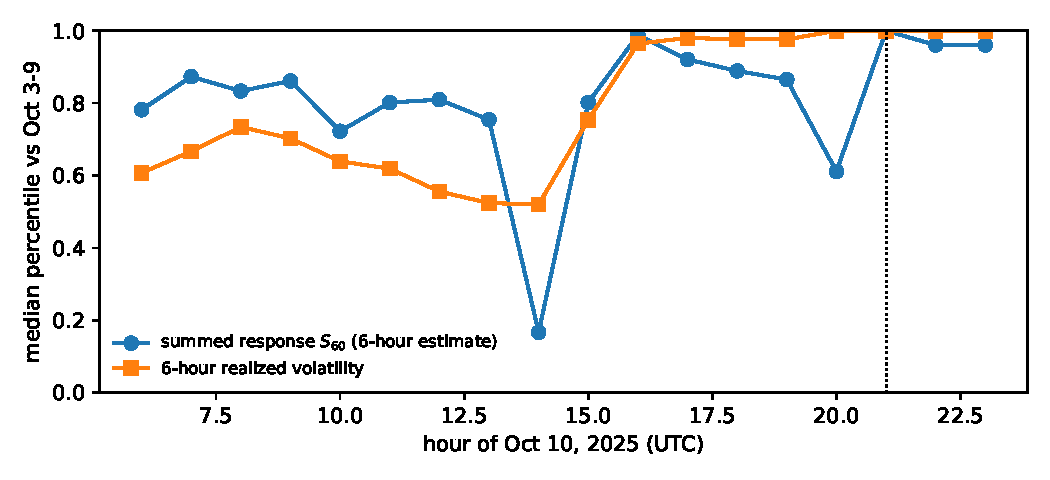
\includegraphics[width=0.72\textwidth]{figs/fig_oct10.pdf}
\caption{October 10, 2025: median percentile, across thin symbols, of the six-hour summed response $S_{60}$ and of six-hour realized volatility, relative to each symbol's October 3--9 distribution. Dotted line: the crash hour (21:00 UTC). Descriptive; the event was chosen after the fact.}\label{fig:oct10}
\end{figure}

Figure~\ref{fig:oct10} shows two things. First, the summed response was elevated through the whole day: in the morning, before volatility rose, the median thin symbol's $S_{60}$ sat at the 72nd to 87th percentile of its previous week, against the 52nd to 73rd for volatility, and at the start of the crash hour 16 of 18 thin symbols with valid estimates were above their previous-week 90th percentile. Second, volatility reached the top of its range from 16:00 onward as well, so on this day the summed response did not warn of anything volatility missed in the final hours; and across symbols it did not rank which coins fell furthest (Spearman $-0.11$, against $+0.36$ for volatility). We draw no inference from one day. The episode is consistent with the thin-book result, an elevated dynamic risk state that sizes excursions rather than timing them, and it illustrates why the paper's claims are about the size of the next hour's excursion, not about predicting crashes.

\subsection{Every pre-registered test}\label{sec:alltests}
Table~\ref{tab:alltests} lists every pre-registered test in this paper, with its outcome and the number of times its test set was opened. Of eleven tests, seven pass and four fail. The failures are in BTCUSDT futures, in BTCUSDT spot, on Bybit with trades alone, and in the six-hour position-sizing backtest. Four passes are in thin Binance books and one in thin US stocks; the certified-guard backtest passes narrowly; and the Bybit test with depth meets its criterion with a negligible effect. Figure~\ref{fig:forest} adds the post-hoc checks.

\begin{table}[t]\centering\small
\begin{threeparttable}
\caption{All pre-registered tests}\label{tab:alltests}
\setlength{\tabcolsep}{3pt}
\begin{tabular}{p{0.3\textwidth}lp{0.27\textwidth}cc}
\toprule
Test (specification hash) & Sample & Primary statistic [CI] & Result & Opened\\
\midrule
BTCUSDT futures, MAE $\mid\hat C_3$ (\texttt{d9521218}) & 2025--26 & $\Delta R^2$ $+0.018$ [$-0.100$, $+0.132$] & fail & 1\\
BTCUSDT spot, MAE $\mid$ amplification (\texttt{b1fd7f8e}) & 2024 & $\Delta R^2$ $-0.023$ [$-0.056$, $-0.002$] & fail & 3\\
Thin books, 10 symbols (\texttt{5910b6b4}) & 2025--26 & $\Delta R^2$ $+1.216$ [$+0.273$, $+7.987$] & pass & 2\\
New thin symbols, 10 (\texttt{6aa8e2c0}) & 2025--26 & $\Delta R^2$ $+0.845$ [$+0.303$, $+6.371$] & pass & 1\\
Fresh days, 20 thin, impact controls (\texttt{65acda36}) & 2025--26 & $\Delta R^2$ $+1.583$ [$+0.588$, $+3.237$] & pass & 1\\
Position sizing, same specification & 2025--26 & $\Delta\log{\rm TLR}$ $-0.017$ [$-0.045$, $+0.011$] & fail & 1\\
Bybit, 14 coins, depth-free & 2025--26 & $\Delta R^2$ $-0.000$ [$-0.001$, $+0.001$] & fail & 1\\
Beyond volatility forecasting, 20 thin (\texttt{71983f1a}) & 2025--26 & $\Delta R^2$ $+2.787$ [$+1.425$, $+4.944$] & pass & 1\\
Certified guard, position sizing (\texttt{b9a56af4}) & 2025--26 & $\Delta\log{\rm TLR}$ $-0.024$ [$-0.051$, $-0.0004$] & pass & 1\\
Bybit with order-book depth, 6 coins (\texttt{ec2145fa}) & 2025--26 & $\Delta R^2$ $+0.033$ [$+0.019$, $+0.053$] & pass & 1\\
Thin US stocks, 23, depth-free (\texttt{f5800a69}) & 2025--26 & $\Delta R^2$ $+0.499$ [$+0.272$, $+0.779$] & pass & 1\\
\bottomrule
\end{tabular}
\begin{tablenotes}\footnotesize\item $\Delta R^2$ in percentage points. ``Opened'' counts executions of the test cell; the repeated openings used unchanged code and specifications (Sections~\ref{sec:x6} and~\ref{sec:spot}). Intervals are 95\%, except 97.5\% for the two fresh-day primaries. \end{tablenotes}
\end{threeparttable}
\end{table}

\begin{figure}[t]\centering
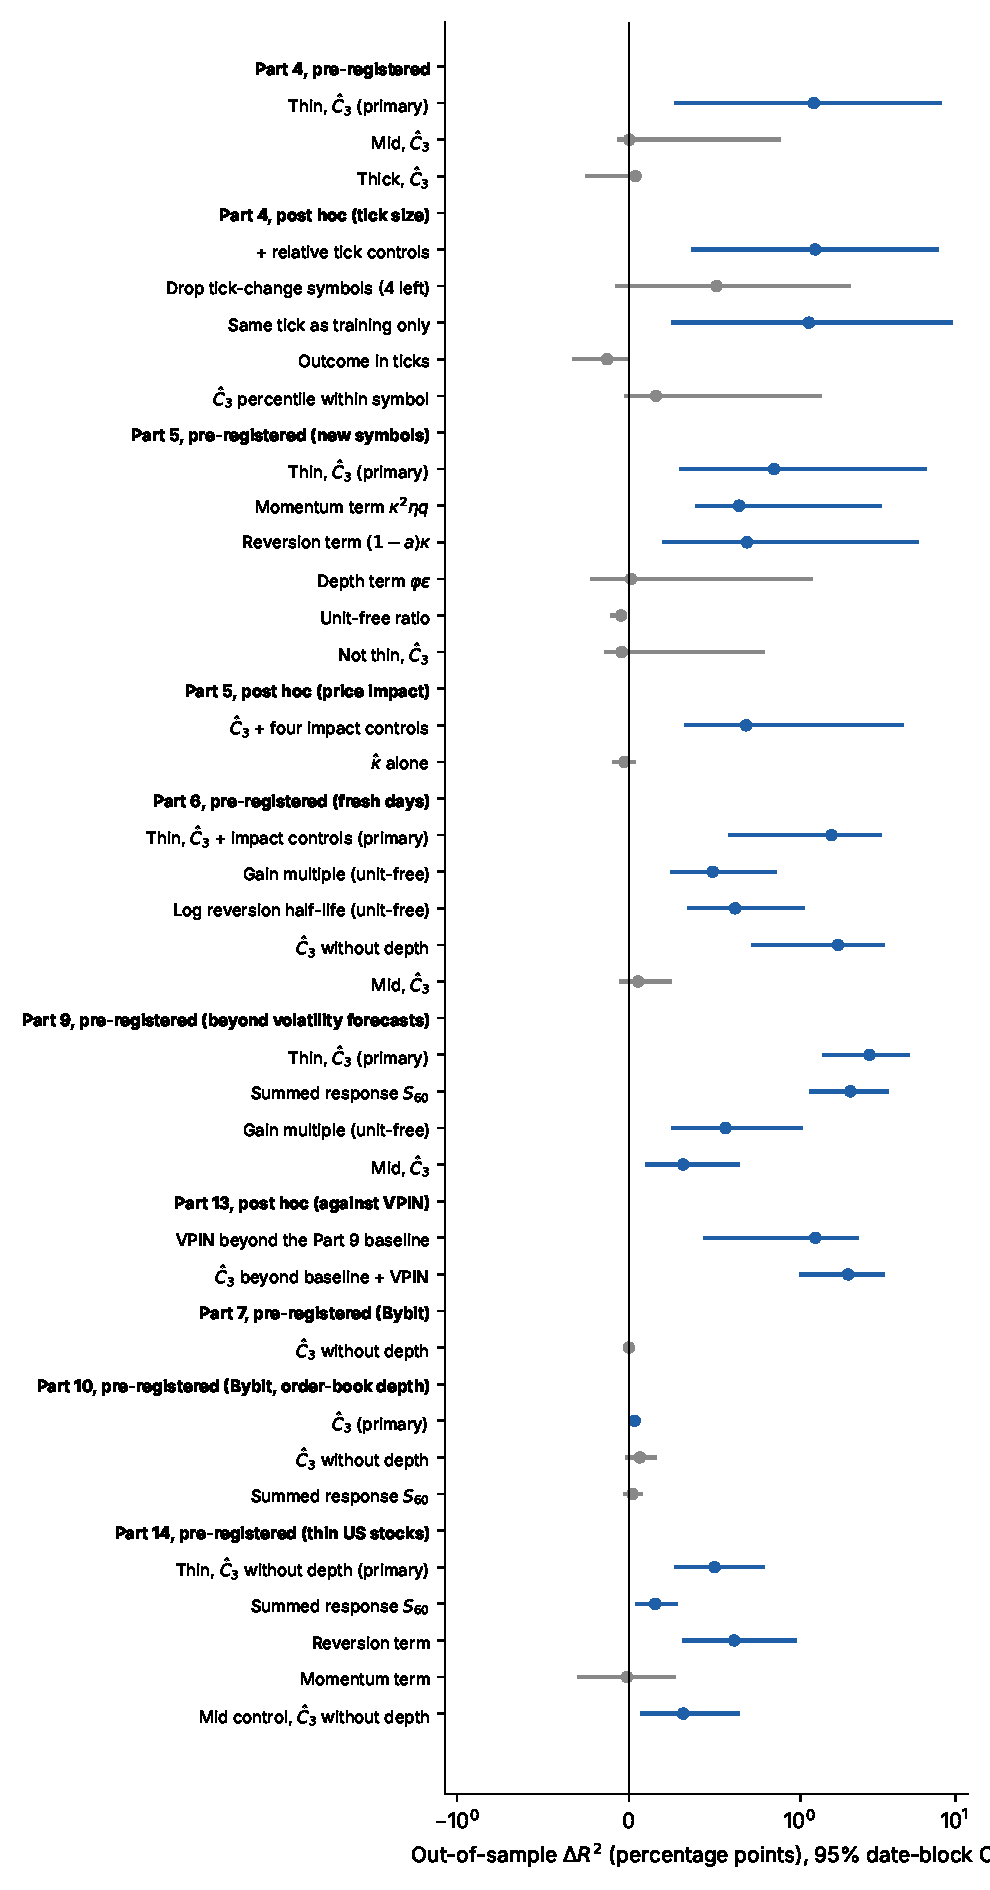
\includegraphics[width=0.78\textwidth]{figs/fig_forest.pdf}
\caption{Every out-of-sample forecasting evaluation in this paper's thin-book program. Points are $\Delta R^2$ in percentage points with date-block bootstrap intervals (symmetric-log axis). Blue: interval above zero. Pre-registered and post-hoc evaluations are grouped separately.}\label{fig:forest}
\end{figure}

\subsection{Threats to validity}\label{sec:threats}
\paragraph{Multiple testing.} The program ran eleven pre-registered primary tests and the post-hoc checks of Figure~\ref{fig:forest}. The six passing forecasting primaries have Clark--West statistics between $5.0$ and $12.6$ (one-sided $p<0.001$ in each), so each survives a Bonferroni correction across all eleven primaries (threshold $0.0045$); statistical significance is not the issue for the Bybit test, its size is. The certified-guard backtest does not survive the correction: its bootstrap one-sided $p$ is about $0.02$, so it is the weakest of the passes. The failures are reported with the same prominence.

\paragraph{Sequential design.} The program was sequential. Each pre-registration fixed one test's specification before its test data were opened, but which test to run next was chosen after the earlier results were known: new symbols after the first pass, impact controls and then a volatility baseline in response to the obvious objections, depth on Bybit after the trade-only test failed, a regulated market after the second venue gave a negligible effect, and a certified operator after the six-hour backtest failed. Pre-registration therefore protects each test from specification search on its own test data; it does not protect the program from choices that adapted across tests. That is why every test is reported, failures included (Figure~\ref{fig:forest}), and why the correction above is taken over all eleven primaries.

\paragraph{Dependence among the passes.} The four passing tests share the 2023--2024 training days, and the original ten thin symbols appear in three of them. They are not four independent replications. They vary three things one at a time: the symbols (Table~\ref{tab:y6}, ten new symbols), the test days (Tables~\ref{tab:z6} and~\ref{tab:z9}, days never used before) and the baseline (impact controls, then a full volatility-forecasting model). The US test (Table~\ref{tab:us}) shares none of their data: a different market, asset class, data source, universe and set of days.

\paragraph{Look-ahead and estimated regressors.} Every feature uses minutes before the forecast hour; winsorization limits, flow scales, $\theta$ and tail thresholds come from training data; and a scrambling audit leaves every hourly feature unchanged when data from $t$ onward are permuted. $\hat C_3$ and $S_{60}$ are estimated from six hours, but the evaluation compares out-of-sample forecasts rather than testing a coefficient, so estimation error in the regressor can only attenuate the measured gain.

\paragraph{Simultaneity.} The structural fits regress the price change on same-minute flow, so $\hat\kappa$ and the depletion slope mix impact with any within-minute response of flow to price. The guard's identification results (Propositions~\ref{prop:invariance} and~\ref{prop:bridge}) concern the impulse response, not these regression coefficients, and the forecasting evidence uses $\hat C_3$ as an index whose value is judged out of sample, not as a causal parameter. Simultaneity therefore changes what $\hat C_3$ measures, not whether the out-of-sample gains are real. We tried to separate the two after the fact by instrumenting this minute's flow with last minute's flow (Part 13, \texttt{R4}), but at the one-minute scale normalized flow is almost serially uncorrelated (median first-stage correlation $0.005$), so the instrument is weak and the instrumented statistic is noise (it adds $0.01$ points of $R^2$, interval including zero). The causal content of $\hat\kappa$ therefore remains open; a convincing instrument would need order-level data.

\paragraph{Selection and survivorship.} The 30 symbols were fixed from one 2024 training day before any T6 statistic was computed, and the new symbols were drawn by a seeded procedure. Symbols had to be listed through 2026, so coins delisted after a collapse are excluded; if anything this removes the episodes in which thin-book risk was largest.

\paragraph{Economic size.} The largest gain, $2.8$ points of $R^2$ on a baseline of $18.6\%$, is a 15\% increase in the explained variance of the next hour's adverse excursion, and tail classification improves by $0.005$ of AUC. In basis points, on the test hours of Table~\ref{tab:z9} and with quintile breakpoints from training data: within each quintile of the volatility forecast, hours in the top quintile of $\hat C_3$ have a next-hour adverse excursion $25.6$ basis points larger than hours in the bottom quintile (date-block 95\% interval $[18.6,32.8]$), against a mean excursion of $112.5$ basis points, and $61$ basis points larger in the most volatile quintile; the share of hours beyond the training 95th percentile rises from $2.3\%$ in the bottom $\hat C_3$ quintile to $5.1\%$ in the top. Unconditional sorts on $S_{60}$ show no pattern; its content appears only with the controls. As a sizing input the gain is worth about a 2.4\% reduction in tail loss per unit of position once the operator is certified (Table~\ref{tab:certguard}). These are modest gains on top of a strong baseline, not a new predictor that replaces volatility.

\paragraph{In margin terms.} To express the 25.6 basis points in the units a risk manager uses, we fit a lognormal distribution to the excursions in each $\hat C_3$ quintile from its mean and median; at one common threshold the fit reproduces the observed share of hours beyond the training 95th percentile in every quintile to within 0.6 percentage points. Shifting the bottom-quintile distribution up by 25.6 basis points, the effect at a given volatility forecast, roughly doubles the probability that a $20\times$ position (liquidated after a 4\% adverse move, with 1\% maintenance margin) is liquidated within the hour, from 1.3\% to 2.7\% (2.3\% to 3.2\% across the interval for the effect). For a $10\times$ position, liquidated after 9\%, the probability almost triples, from 0.04\% to 0.11\%. On \$1M of notional at $20\times$, the extra expected loss of margin is about \$710 per hour held (\$490 to \$960; \texttt{recompute\_dollar.py}). These figures come from a fitted distribution, not a test, and they treat the hour's excursion from its opening price as the liquidation trigger. They show that a difference that is small in basis points is large in the tail that leverage makes relevant, which is where a pre-trade control operates.

\paragraph{Venue.} The size of the result depends on the venue. It is largest in thin Binance USD-M books; in thin US stocks it passes a pre-registered test at about a fifth of that size, and it also appears in mid-size US stocks (Table~\ref{tab:us}); on Bybit it failed with trade data alone and, with order-book depth, met its pre-registered criterion with an effect about one eightieth of Binance's (Table~\ref{tab:bybitob}).

\subsection{What the evidence says}\label{sec:thin_summary}
Deep books sit on the stable side of the amplification condition. Flow depletes the side it hits on a fixed price grid, although re-centred depth bands make it look like replenishment, and we observe no peak overshoot. In thin Binance books the condition is still negative on average but binds more often, and the six-hour estimates of cumulative transient risk forecast the size of the next hour's adverse excursion out of sample. Four pre-registered tests pass, on the original symbols, on ten new symbols, on fresh days with price-impact controls, and on fresh days beyond a full volatility-forecasting baseline, where the gain is largest ($+2.8$ points of $R^2$) and extends to tail classification. The summed response $S$ of Proposition~\ref{prop:sum}, the guard's own statistic, carries the same information, and unit-free versions work. The content does not run through depth depletion, and in Binance books it is much weaker at mid depth and absent in BTCUSDT. In thin US stocks a fifth pre-registered forecasting test passes, at about a fifth of the Binance size and with a gain in mid-size stocks too; on Bybit the statistic is absent with trades alone and negligible with depth; and as a position-sizing input it improves a volatility limit only modestly once the operator is certified. Thin books are risky because their prices revert too slowly relative to the impact and momentum of the flow that moves them, which is what $S=\tilde\kappa/(m-q\tilde\kappa)$ measures.
\section{Policy implications}\label{sec:policy}

\paragraph{Pre-trade controls.} Rule 15c3-5 requires pre-trade controls that prevent orders exceeding credit or capital thresholds \citep{sec2010}. Static single-order caps and daily value-at-risk limits do not see transient dynamics. Theorem~\ref{thm:guard} identifies the quantity that a solvency-motivated control should bound: inventory times the shock envelope times the summed absolute impulse response. Peak-based or eigenvalue-based limits are either unsafe or blind in exactly the regimes where they matter. Our evidence locates where such controls matter. In the deepest crypto book the amplifying regime is rare and the statistic carries no forecasting value; in thin books it is more frequent, and six-hour estimates of the summed response forecast the next hour's adverse excursion beyond volatility forecasts and price impact (Section~\ref{sec:thin}). Our backtests also set a limit on what such a control can do with public data. A six-hour estimate of the summed response adds nothing to a volatility limit as a sizing input (Table~\ref{tab:backtest}); an operator certified from three days of data improves a volatility limit modestly, by 2.4\% in tail loss per unit of position (Table~\ref{tab:certguard}); and limits built on the estimate alone do worse than volatility in both. The guard's role is therefore a ceiling on worst-case loss under a certified operator and a correction to conventional volatility limits, not a replacement for them, and it is most relevant for books with under about \$0.4M of depth within 1\% of the mid.

\paragraph{Pricing reversion.} Proposition~\ref{prop:equil} shows that dealers under-supply reversion because its benefit, lower tail exposure for every leveraged position, is not paid to them. Maker rebates are a natural instrument: a rebate that rises with the book's summed response, $(1-\theta/N)\Lambda S^2/\tilde\kappa$ per unit of reversion, prices the externality with an observable. Venues already tier rebates by volume; tiering them by contribution to reversion in thin books is a design question our model makes precise.

\paragraph{Market design.} Frequent batch auctions remove latency races within a batch \citep{budish2015}. Transient amplification, when it exists, operates over many seconds and spans many batches, so batching and a state-carrying guard address different failures and can be complements.

\paragraph{Supervision without identification.} The companion paper shows that identifying algorithms from public data is expensive: any risk limit that depends on individual cohort memory rates $\eta_i$ separately from the aggregate impulse response $(h_k)_{k\ge 0}$ is either unidentifiable from public prices under passive observation (where only the merged rate--weight measure $\mathcal M$ is identified) or inherits the ill-conditioned minimax sample complexity $(\Delta\eta)^{-(4K-2)}$ (and $(\log N)^{-1}$ for general completely monotone memory). By contrast, the guard needs only aggregate impulse coefficients and operator confidence sets, which are invariant to how flow is split across cohorts (Propositions~\ref{prop:invariance} and~\ref{prop:bridge}). When class-tagged disclosure is available, the companion paper's sample-efficiency gain of order $(\Delta\eta)^{-(4K-4)}$ shrinks the estimation confidence radius $\Delta G(\tau)$ in Theorem~\ref{thm:robust} by a factor of order $(\Delta\eta)^{-(2K-2)}$, reducing the robust admission haircut $\tau\Delta G(\tau)$ without active market probing (which would itself consume $\kappa\|u\|_{\ell_1}$ of the transient excursion budget). Supervisors can therefore ask venues and brokers to report summed-gain statistics and their confidence radii instead of attempting to infer black-box learners. Our results argue for reporting impact, mean reversion and refill directly, because those are the primitives that decide whether a book can amplify. They also show that feedback and amplification are different objects: measured feedback is largest in the deepest books, where amplification is rarest (Table~\ref{tab:x3}).

\section{Conclusion}\label{sec:conclusion}

The theory answers three questions. A book amplifies when depletion outweighs impact-weighted reversion; with momentum the one-period margin is sufficient but not exact, and momentum alone cannot make a stable book overshoot. Cumulative risk is long-run impact divided by reversion net of momentum, and the guard that bounds it is the largest safe pre-trade rule, computable and identified from public data. In equilibrium reversion is under-supplied, and the corrective price is a function of the guard's own statistic.

The evidence is mixed in an informative way. The deepest crypto book sits on the stable side of the condition; flow depletes the side it hits on a fixed price grid, but not enough to produce a peak overshoot in the data we observe. In thin Binance books, six-hour estimates of cumulative transient risk forecast the size of the next hour's adverse excursion out of sample in four pre-registered tests, in unit-free form, beyond price impact and beyond a full volatility-forecasting baseline. At a given volatility forecast, hours in the top quintile of the statistic have next-hour excursions about 26 basis points larger than hours in the bottom quintile. In thin US stocks, with consolidated trades, the statistic passes a fifth pre-registered test at about a fifth of the Binance size, and appears in mid-size stocks too. On Bybit it is absent with trades alone and negligible with order-book depth, the effect is much weaker in deeper Binance books, and as a sizing input it helps only once the operator is certified from days of data, and then modestly. Thin books are risky because their prices revert too slowly relative to the impact and momentum of the flow that moves them.

Three extensions would settle what remains open. Message-level data from a regulated market, such as LOBSTER or TAQ for US equities, would extend the US test to depth and to large stocks, show where the effect ends, and allow depletion to be measured without the recentering of band depth. Data on liquidity-provider identities would test the equilibrium's prediction that fewer dealers mean more transient risk. And longer certification windows, or certification with order-level data, would show whether the modest gain of a certified guard over volatility limits can be made large.

\paragraph{Data and code availability.} All data are public: Binance archives (\url{https://data.binance.vision}), verified against published checksums, and Bybit's order-book history (\url{https://www.bybit.com/derivatives/en/history-data}) and trade archive (\url{https://public.bybit.com}); US consolidated trades are from the Alpaca market-data API (\url{https://alpaca.markets}, free account). Pre-registered specifications, their SHA-256 hashes and test-set unlock counters are in the replication package. Each number is produced by a notebook cell or script that writes a result file (Appendix~\ref{app:repro}).

\paragraph{Use of AI tools.} The authors used Claude (Anthropic), an AI assistant, to write and debug analysis code, run checks of derivations and numerical results, and draft and edit text. Every number in the paper is produced by code the authors executed and archived in the replication package. The authors reviewed all content and take full responsibility for it.

\paragraph{Disclosures.} The authors declare no relevant financial interests.
\begin{thebibliography}{99}\setlength{\itemsep}{2pt}\small
\bibitem[21Shares(2025)]{shares2025} 21Shares (2025). Record crypto liquidations amid tariff shock. Research note, October 13, 2025. \url{https://www.21shares.com/research/record-crypto-liquidations-amid-tariff-shock}.
\bibitem[Almgren and Chriss(2001)]{almgren2001} Almgren, R., and N. Chriss (2001). Optimal execution of portfolio transactions. \emph{Journal of Risk} 3, 5--39.
\bibitem[Amihud(2002)]{amihud2002} Amihud, Y. (2002). Illiquidity and stock returns: Cross-section and time-series effects. \emph{Journal of Financial Markets} 5, 31--56.
\bibitem[Andersen and Bondarenko(2014)]{andersen2014} Andersen, T. G., and O. Bondarenko (2014). VPIN and the flash crash. \emph{Journal of Financial Markets} 17, 1--46.
\bibitem[Avellaneda and Stoikov(2008)]{avellaneda2008} Avellaneda, M., and S. Stoikov (2008). High-frequency trading in a limit order book. \emph{Quantitative Finance} 8, 217--224.
\bibitem[Biais et~al.(2005)]{biais2005} Biais, B., L. Glosten, and C. Spatt (2005). Market microstructure: A survey of microfoundations, empirical results, and policy implications. \emph{Journal of Financial Markets} 8, 217--264.
\bibitem[Biais et~al.(1995)]{biais1995} Biais, B., P. Hillion, and C. Spatt (1995). An empirical analysis of the limit order book and the order flow in the Paris Bourse. \emph{Journal of Finance} 50, 1655--1689.
\bibitem[Bouchaud et~al.(2004)]{bouchaud2004} Bouchaud, J.-P., Y. Gefen, M. Potters, and M. Wyart (2004). Fluctuations and response in financial markets: The subtle nature of ``random'' price changes. \emph{Quantitative Finance} 4, 176--190.
\bibitem[Bouchaud et~al.(2018)]{bouchaud2018} Bouchaud, J.-P., J. Bonart, J. Donier, and M. Gould (2018). \emph{Trades, Quotes and Prices: Financial Markets Under the Microscope}. Cambridge University Press.
\bibitem[Brogaard et~al.(2014)]{brogaard2014} Brogaard, J., T. Hendershott, and R. Riordan (2014). High-frequency trading and price discovery. \emph{Review of Financial Studies} 27, 2267--2306.
\bibitem[Brunnermeier and Pedersen(2009)]{brunnermeier2009} Brunnermeier, M. K., and L. H. Pedersen (2009). Market liquidity and funding liquidity. \emph{Review of Financial Studies} 22, 2201--2238.
\bibitem[Budish et~al.(2015)]{budish2015} Budish, E., P. Cramton, and J. Shim (2015). The high-frequency trading arms race: Frequent batch auctions as a market design response. \emph{Quarterly Journal of Economics} 130, 1547--1621.
\bibitem[Cartea et~al.(2015)]{cartea2015} Cartea, \'A., S. Jaimungal, and J. Penalva (2015). \emph{Algorithmic and High-Frequency Trading}. Cambridge University Press.
\bibitem[Cespa and Foucault(2014)]{cespa2014} Cespa, G., and T. Foucault (2014). Illiquidity contagion and liquidity crashes. \emph{Review of Financial Studies} 27, 1615--1660.
\bibitem[Clark and West(2007)]{clark2007} Clark, T. E., and K. D. West (2007). Approximately normal tests for equal predictive accuracy in nested models. \emph{Journal of Econometrics} 138, 291--311.
\bibitem[Cont et~al.(2014)]{cont2014} Cont, R., A. Kukanov, and S. Stoikov (2014). The price impact of order book events. \emph{Journal of Financial Econometrics} 12, 47--88.
\bibitem[Corsi(2009)]{corsi2009} Corsi, F. (2009). A simple approximate long-memory model of realized volatility. \emph{Journal of Financial Econometrics} 7, 174--196.
\bibitem[Dahleh and Diaz-Bobillo(1995)]{dahleh1995} Dahleh, M. A., and I. J. Diaz-Bobillo (1995). \emph{Control of Uncertain Systems: A Linear Programming Approach}. Prentice Hall.
\bibitem[Dahleh and Pearson(1987)]{dahleh1987} Dahleh, M. A., and J. B. Pearson (1987). $\ell^1$-optimal feedback controllers for MIMO discrete-time systems. \emph{IEEE Transactions on Automatic Control} 32, 314--322.
\bibitem[Degryse et~al.(2005)]{degryse2005} Degryse, H., F. de Jong, M. van Ravenswaaij, and G. Wuyts (2005). Aggressive orders and the resiliency of a limit order market. \emph{Review of Finance} 9, 201--242.
\bibitem[Diebold and Mariano(1995)]{diebold1995} Diebold, F. X., and R. S. Mariano (1995). Comparing predictive accuracy. \emph{Journal of Business \& Economic Statistics} 13, 253--263.
\bibitem[Easley et~al.(2012)]{easley2012} Easley, D., M. M. L\'opez de Prado, and M. O'Hara (2012). Flow toxicity and liquidity in a high-frequency world. \emph{Review of Financial Studies} 25, 1457--1493.
\bibitem[Foucault et~al.(2005)]{foucault2005} Foucault, T., O. Kadan, and E. Kandel (2005). Limit order book as a market for liquidity. \emph{Review of Financial Studies} 18, 1171--1217.
\bibitem[Harvey(2017)]{harvey2017} Harvey, C. R. (2017). Presidential address: The scientific outlook in financial economics. \emph{Journal of Finance} 72, 1399--1440.
\bibitem[Harvey et~al.(2016)]{harvey2016} Harvey, C. R., Y. Liu, and H. Zhu (2016). \ldots and the cross-section of expected returns. \emph{Review of Financial Studies} 29, 5--68.
\bibitem[Hendershott et~al.(2011)]{hendershott2011} Hendershott, T., C. M. Jones, and A. J. Menkveld (2011). Does algorithmic trading improve liquidity? \emph{Journal of Finance} 66, 1--33.
\bibitem[Ho and Stoll(1981)]{ho1981} Ho, T., and H. R. Stoll (1981). Optimal dealer pricing under transactions and return uncertainty. \emph{Journal of Financial Economics} 9, 47--73.
\bibitem[Holm(1979)]{holm1979} Holm, S. (1979). A simple sequentially rejective multiple test procedure. \emph{Scandinavian Journal of Statistics} 6, 65--70.
\bibitem[Huang and Wang(2009)]{huang2009} Huang, J., and J. Wang (2009). Liquidity and market crashes. \emph{Review of Financial Studies} 22, 2607--2643.
\bibitem[Jord\`a(2005)]{jorda2005} Jord\`a, \`O. (2005). Estimation and inference of impulse responses by local projections. \emph{American Economic Review} 95, 161--182.
\bibitem[J.P. Morgan/Reuters(1996)]{riskmetrics1996} J.P. Morgan/Reuters (1996). \emph{RiskMetrics---Technical Document}, 4th ed. New York: J.P. Morgan.
\bibitem[Kirilenko et~al.(2017)]{kirilenko2017} Kirilenko, A., A. S. Kyle, M. Samadi, and T. Tuzun (2017). The Flash Crash: High-frequency trading in an electronic market. \emph{Journal of Finance} 72, 967--998.
\bibitem[Kreiss(1962)]{kreiss1962} Kreiss, H.-O. (1962). \"Uber die Stabilit\"atsdefinition f\"ur Differenzengleichungen die partielle Differentialgleichungen approximieren. \emph{BIT Numerical Mathematics} 2, 153--181.
\bibitem[K\"unsch(1989)]{kunsch1989} K\"unsch, H. R. (1989). The jackknife and the bootstrap for general stationary observations. \emph{Annals of Statistics} 17, 1217--1241.
\bibitem[Kyle(1985)]{kyle1985} Kyle, A. S. (1985). Continuous auctions and insider trading. \emph{Econometrica} 53, 1315--1335.
\bibitem[Kyle and Obizhaeva(2016)]{kyle2016} Kyle, A. S., and A. A. Obizhaeva (2016). Market microstructure invariance: Empirical hypotheses. \emph{Econometrica} 84, 1345--1404.
\bibitem[Large(2007)]{large2007} Large, J. (2007). Measuring the resiliency of an electronic limit order book. \emph{Journal of Financial Markets} 10, 1--25.
\bibitem[Makarov and Schoar(2020)]{makarov2020} Makarov, I., and A. Schoar (2020). Trading and arbitrage in cryptocurrency markets. \emph{Journal of Financial Economics} 135, 293--319.
\bibitem[Menkveld(2013)]{menkveld2013} Menkveld, A. J. (2013). High frequency trading and the new market makers. \emph{Journal of Financial Markets} 16, 712--740.
\bibitem[Newey and West(1987)]{newey1987} Newey, W. K., and K. D. West (1987). A simple, positive semi-definite, heteroskedasticity and autocorrelation consistent covariance matrix. \emph{Econometrica} 55, 703--708.
\bibitem[Niroula and Niroula(2026)]{niroula2026} Niroula, P., and P. Niroula (2026). Auditable memory and financial identification limits in electronic limit order books. Working paper, Minnesota State University, Mankato.
\bibitem[Nosek et~al.(2018)]{nosek2018} Nosek, B. A., C. R. Ebersole, A. C. DeHaven, and D. T. Mellor (2018). The preregistration revolution. \emph{Proceedings of the National Academy of Sciences} 115, 2600--2606.
\bibitem[Obizhaeva and Wang(2013)]{obizhaeva2013} Obizhaeva, A. A., and J. Wang (2013). Optimal trading strategy and supply/demand dynamics. \emph{Journal of Financial Markets} 16, 1--32.
\bibitem[Schneider and Lillo(2019)]{schneider2019} Schneider, M., and F. Lillo (2019). Cross-impact and no-dynamic-arbitrage. \emph{Quantitative Finance} 19, 137--154.
\bibitem[SEC(2010)]{sec2010} U.S. Securities and Exchange Commission (2010). Risk management controls for brokers or dealers with market access. Release No.\ 34-63241.
\bibitem[Shleifer and Vishny(1992)]{shleifer1992} Shleifer, A., and R. W. Vishny (1992). Liquidation values and debt capacity: A market equilibrium approach. \emph{Journal of Finance} 47, 1343--1366.
\bibitem[Sornette et~al.(2023)]{sornette2023} Sornette, D., S. Lera, J. Lin, and K. Wu (2023). Non-normal interactions create socio-economic bubbles. \emph{Communications Physics} 6, 261.
\bibitem[Spijker(1991)]{spijker1991} Spijker, M. N. (1991). On a conjecture by LeVeque and Trefethen related to the Kreiss matrix theorem. \emph{BIT Numerical Mathematics} 31, 551--555.
\bibitem[Trefethen and Embree(2005)]{trefethen2005} Trefethen, L. N., and M. Embree (2005). \emph{Spectra and Pseudospectra: The Behavior of Nonnormal Matrices and Operators}. Princeton University Press.
\bibitem[van~Waarde et~al.(2020)]{vanwaarde2020} van~Waarde, H. J., J. Eising, H. L. Trentelman, and M. K. Camlibel (2020). Data informativity: A new perspective on data-driven analysis and control. \emph{IEEE Transactions on Automatic Control} 65, 5153--5168.
\bibitem[Vidyasagar(1986)]{vidyasagar1986} Vidyasagar, M. (1986). Optimal rejection of persistent bounded disturbances. \emph{IEEE Transactions on Automatic Control} 31, 527--534.
\end{thebibliography}

\appendix
\section{Proofs}\label{app:proofs}

\paragraph{Proposition~\ref{prop:jury}.} With one cohort, $J=\begin{psmallmatrix}a&\kappa q\\ \eta a&1-\eta+\eta\kappa q\end{psmallmatrix}$, so ${\rm tr}J=a+1-\eta+\eta\kappa q$ and $\det J=a(1-\eta)$. The Jury conditions for a real $2\times2$ matrix are $|\det J|<1$ and $1\pm{\rm tr}J+\det J>0$. Substituting $a=1-\kappa\varphi_f$: $1-{\rm tr}J+\det J=\eta(1-a-\kappa q)=\eta\kappa(\varphi_f-q)$, positive iff $q<\varphi_f$; and $1+{\rm tr}J+\det J=(4-2\eta)-\kappa[(2-\eta)\varphi_f-\eta q]$, positive iff the stated bound on $\kappa$ holds (automatically when $(2-\eta)\varphi_f\le\eta q$).

\paragraph{Proposition~\ref{prop:invariance}.} Equal merged measures give equal $G$, hence equal $H$, and the impulse coefficients are the Laurent coefficients of $H$ (companion paper, Theorem on merged equivalence). Under $z\mapsto Tz$, $c^\top J^kb$ is unchanged because $CT^{-1}(TJT^{-1})^kTb=CJ^kb$, while the row norm $\|CT^{-1}(TJT^{-1})^k\|$ depends on $T$. The displayed price path is the convolution of inputs with $\{g_k\}$, and its worst case over the $\ell_\infty$ ball is $\bar u\sum|g|$ by H\"older.

\paragraph{Theorem~\ref{thm:radius}.} (i) $\sup_t\|CJ^tz_0\|\le\sup_t\|CJ^t\|\|z_0\|$, with equality approached by aligning $z_0$ with the top right singular vector of $CJ^{t^*}$ at the maximizing $t^*$. (ii) The Kreiss matrix theorem with Spijker's sharp constant gives $\mathcal K(J)\le\sup_t\|J^t\|\le en\mathcal K(J)$; substitute in (i). (iii) Take $J_\theta=\begin{psmallmatrix}\rho&\theta\\0&\rho/2\end{psmallmatrix}$; then $\rho(J_\theta)=\rho$ and $(1,0)J_\theta e_2=\theta$, so $M_C\ge|\theta|$ and $r^*_{\rm exact}\le B/|\theta|\to0$.

\paragraph{Proposition~\ref{prop:multi}.} With all blocks entrywise nonnegative, every entry of $J_{\rm multi}^t$ is a polynomial in the entries of $K_{21}$ with nonnegative coefficients, so it is non-decreasing in $K_{21}$; with $C\ge0$, so is every entry of $CJ^t$ and hence its norm. For the Kreiss constant, the Neumann series gives $|(zI-J)^{-1}|\le(|z|I-J)^{-1}$ entrywise for $|z|>1$, so the supremum is attained on the real axis, where $(rI-J)^{-1}=\sum_kJ^k/r^{k+1}$ is entrywise non-decreasing in $K_{21}$.

\paragraph{Proposition~\ref{prop:shape}.} The recursion \eqref{eq:rec} is solved by $h_k=Aa^k+Bb^k$ with $B(b-a)=\varphi\varepsilon$ and $A+B=\kappa$. Setting the derivative of $Aa^k+Bb^k$ in $k$ to zero gives the unique critical point $k^*$; since the function rises at first ($h_1>h_0$) and tends to zero, $k^*$ is its maximum on $[0,\infty)$, and a unimodal function attains its maximum over the integers at $\lfloor k^*\rfloor$ or $\lceil k^*\rceil$. Summing \eqref{eq:rec} over $k\ge1$ gives $S=\kappa+aS+\varphi\varepsilon/r$, so $S=(\kappa+\varphi\varepsilon/r)/(1-a)$, decreasing in $r$ when $\varphi\varepsilon>0$.

\paragraph{Theorem~\ref{thm:forward}.} After the step, inventory is at most $|I^{\rm post}_{t+1}(\alpha_t)|$ in absolute value. The price move over the step and the cumulative window is bounded by $M_C\|z_t\|_2$ (drift from the current state) plus $s(\alpha)G_{\rm cum}\bar u_{\rm cum}$ (admitted shocks), by superposition and H\"older. The margin requirement scales the loss by $(1+\mu)$. Hedging cost and the post-fill margin increment are deducted directly. Inequality \eqref{eq:guardineq} therefore implies $B_{{\rm rem},t+1}\ge R_{\rm safe}$ for every admissible disturbance, and induction over steps at which an admissible $\alpha$ exists gives forward solvency. Setting $\alpha=0$ ($M_C(0)=1$, no fills, no hedge) gives $\bar u_{\rm adm}$. Sufficiency over the Euclidean ball follows from the norm bounds. When $z_t=0$ the remaining shock term is attained by $u=-{\rm sign}(I)\bar u$, which gives necessity; when $z_t\ne0$ the drift bound $M_C\|z_t\|_2$ need not be attained, so the condition is sufficient but not necessary.

\paragraph{Proposition~\ref{prop:dominance}.} The eigenvalue rule admits $\alpha_\rho$; a one-step breach occurs at $\alpha_\rho$ exactly when the left side of \eqref{eq:guardineq} with $G_{\rm cum}$ replaced by the one-step gain exceeds $B_{{\rm rem},t}$, which rearranges to the stated inequality. The summed-gain guard admits only levels satisfying \eqref{eq:guardineq}, so it never admits the breaching level, and by the feasibility assumption it admits at least $\alpha=0$.

\paragraph{Proposition~\ref{prop:lucas}.} The steady-state gain is $\eta=P/(P+\sigma_\nu^2)$ with $P$ the positive root of $P^2-\sigma_\zeta^2P-\sigma_\zeta^2\sigma_\nu^2=0$. Since $P$ is strictly increasing in $\sigma_\zeta^2$ and $\eta$ is strictly increasing in $P$, $\eta^*$ is strictly increasing in $\sigma_\zeta^2(\alpha)=\alpha^2\sigma_{\zeta,0}^2$, hence in $\alpha$. The second statement is immediate under the stated monotonicity.

\section{Notation}\label{app:notation}
\begin{longtable}{p{0.2\textwidth}p{0.7\textwidth}}
\toprule
Symbol & Meaning\\
\midrule
\endhead
$x_t,\ d_t,\ u_t$ & price displacement, depth imbalance $(B-A)/(B+A)$, signed flow\\
$a,\ \kappa$ & price persistence and direct impact\\
$\varphi,\ \varepsilon,\ r$ & price sensitivity to depth, depletion per unit of flow, refill rate\\
$\eta,\ q$ & momentum memory rate and aggressiveness\\
$C_2,\ C_3$ & amplification statistics $\varphi\varepsilon-(1-a)\kappa$ and $C_2+\kappa^2\eta q$\\
$h_k,\ g_k$ & impulse response of the book; price impulse coefficient of the controlled system\\
$J(\alpha)$ & closed-loop operator at admission level $\alpha$\\
$M_C,\ G_{\rm cum}$ & peak and summed price-row gains\\
$\mathcal K(J)$ & Kreiss constant\\
$\bar u,\ \bar u_{\rm step},\ \bar u_{\rm cum}$ & shock envelopes\\
$B_{\rm rem},\ R_{\rm safe},\ \mu$ & remaining margin buffer, safety reserve, maintenance-margin rate\\
$\epsilon,\ S$ & operator confidence radius and $\sum_k\|J^k\|$\\
$M_{\rm std},\ A_{xx}$ & unit-free and price-to-price spot amplification statistics\\
\bottomrule
\end{longtable}

\section{Additional material}\label{app:ia}

\subsection{Specification of the pre-registered tests}
\paragraph{Futures (Table~\ref{tab:d8}).} Question: does $\hat C_3$, estimated from the previous six hours of futures depth, flow and price, predict the next hour's MAE beyond controls? Unit: hourly blocks 06--23 UTC, features from $[t-360,t)$ minutes, outcomes from $(t,t+60]$. Controls: $rv_{60}$, $rv_{360}$, $|r_{60}|$, flow imbalance, log volume, log depth, imbalance, open-interest change. Model: OLS; tail is the outcome above the training 90th percentile; score is the fitted value. Inference: Clark--West with Newey--West (6 lags); day-block bootstrap with 2,000 draws. Secondary: peak ratio as candidate; open-interest drop and depth collapse as outcomes; Holm. Train $\le$ 2024-12-31; test $\ge$ 2025-01-01. Hash \texttt{d95212187ae42052591a5ca5acf73317} \texttt{0f217f430a5a6ca812da6e48a1e4af85}; one unlock.

\paragraph{Spot (Section~\ref{sec:spot}).} Question: does pre-window $A_{xx}$ predict the next ten minutes' MAE beyond volatility and flow controls? Unit: non-overlapping 30-minute blocks; features from the previous ten minutes. Controls: $rv_{10m}$, $rv_{60m}$, $|r_{10m}|$, flow imbalance, log volume, spectral radius, hour of day. Train 2021--2023; test 2024. Hash \texttt{b1fd7f8eef15df1ba295eb6d32b53be6} \texttt{c23ea2d23c5216de912555e62716e5ae}; three unlocks (see text).

\section{Reproducibility: source of every number}\label{app:repro}

The replication package contains numbered Colab notebooks and stand-alone scripts; its README lists them in run order. ``Part $N$'' below and in table notes refers to notebook $N$ (Part 1: theorem checks and spot tests; Part 2: BTCUSDT futures depth; Parts 4--14: the cross-section, replications, fresh-day tests, second venues, the CFTC test, the certified guard, post-hoc checks and US equities). Result identifiers such as \texttt{X6} or \texttt{U6} name the JSON file that the notebook writes. ``Kind'' distinguishes closed-form or simulation results (recomputed), results from public market data (real data), and audits.

\begin{longtable}{p{0.37\textwidth}p{0.37\textwidth}p{0.14\textwidth}}
\toprule
Result & Source & Kind\\
\midrule
\endhead
Spectral blindness gains & \texttt{T5\_spectral\_blindness} & recomputed\\
Table~\ref{tab:kreiss}; burst operator gain, $q$, certificate & \texttt{kreiss\_table.py} $\to$ \texttt{R\_P2\_kreiss.json} & recomputed\\
Table~\ref{tab:calib}, Figure~\ref{fig:calib} & \texttt{calib\_guard.py} $\to$ \texttt{R\_P2\_calibrated\_guard.json} & recomputed\\
Figure~\ref{fig:pseudo} & \texttt{make\_figs2.py} & recomputed\\
Theorem~\ref{thm:t6}, Propositions~\ref{prop:shape}, \ref{prop:t6m} draws & \texttt{T6\_amplification\_theorem} & recomputed\\
Guard maximality; peak guard unsafe; monotonicity & \texttt{T7\_guard\_maximality}, \texttt{P2.11-T1} & recomputed\\
Robust gain, 30,000 draws & \texttt{T8\_robust\_gain} & recomputed\\
Operator ball coverage; certificate share & \texttt{P2.4-T1\_coverage} & recomputed\\
Summed gain vs.\ weights & \texttt{T9\_bridge} & recomputed\\
Depth validation (Table~\ref{tab:d2}) & \texttt{D2\_depth\_validation} & real data\\
Table~\ref{tab:d3} & \texttt{D3\_T6\_structural\_train} & real data\\
Figure~\ref{fig:med}, Table~\ref{tab:d4} & \texttt{D4\_depth\_mediation\_train} & real data\\
No-look-ahead audit & \texttt{D5\_no\_lookahead} & audit\\
Table~\ref{tab:d8}; hash & \texttt{D8\_depth\_test\_G2}, \texttt{P2\_depth.json} & real data\\
Flag comparison & \texttt{D8b\_flag\_comparison} & real data\\
Table~\ref{tab:d9}, Figure~\ref{fig:events} & \texttt{D9\_event\_studies} & real data\\
Unit dependence $8.73\to86{,}731$ & \texttt{P2.2-T1\_unit\_invariance} & real data\\
Table~\ref{tab:spotnull}; sensitivity & \texttt{P2.2-T2}, \texttt{T3}, \texttt{T4}, \texttt{T5} & real data\\
Table~\ref{tab:spotlp} & \texttt{T6-E\_overshoot\_real} & real data\\
Spot predictive test & \texttt{P2.5\_predictive\_G2}, \texttt{P2.5-T2}, \texttt{T3} & real data\\
Spot flag comparison & \texttt{P2.7-T2\_vol\_ablation} & real data\\
Proposition~\ref{prop:sum}; Remark~\ref{rem:counter}; Theorem~\ref{thm:nomom} check & \texttt{equilibrium.py}, \texttt{t6m\_search*.py}, \texttt{thmA\_check.py} & recomputed\\
Proposition~\ref{prop:equil} numbers & \texttt{equilibrium.py} $\to$ \texttt{R\_P2\_equilibrium.json} & recomputed\\
Proposition~\ref{prop:invariance} check; multi-asset example; Proposition~\ref{prop:lucas} check & \texttt{recompute\_oct20.py} & recomputed\\
Tables~\ref{tab:x3}, \ref{tab:x4}, \ref{tab:x8}; tick events & Part 4: \texttt{X3}, \texttt{X4}, \texttt{X8}, \texttt{X7} & real data\\
Table~\ref{tab:x6}; flags & Part 4: \texttt{X6\_xsec\_test\_G2}, \texttt{X6b}; \texttt{P4\_xsec.json} (5910b6b4\ldots) & real data\\
Table~\ref{tab:x6r} & Part 4: \texttt{X6r\_robustness\_posthoc} & real data (post hoc)\\
Table~\ref{tab:y6} & Part 5: \texttt{Y6\_replication\_G2}; \texttt{P5\_replication.json} (6aa8e2c0\ldots) & real data\\
Table~\ref{tab:y8} & Part 5: \texttt{Y8\_kappa\_control\_posthoc} & real data (post hoc)\\
Tables~\ref{tab:z6}, \ref{tab:backtest}; equilibrium check & Part 6: \texttt{Z6\_*}, \texttt{Z8}; \texttt{P6\_fresh\_days.json} (65acda36\ldots) & real data\\
Table~\ref{tab:certguard}, Figure~\ref{fig:oct10}, economic size (Section~\ref{sec:threats}) & Part 12: \texttt{Q6\_certified\_guard}, \texttt{Q7\_oct10\_event}, \texttt{E1\_economic\_size}; \texttt{P12\_certified\_guard.json} (b9a56af4\ldots) & real data\\
Liquidation probabilities and dollar losses (Section~\ref{sec:threats}) & \texttt{recompute\_dollar.py} (from \texttt{E1\_economic\_size}) $\to$ \texttt{R\_P2\_dollar\_translation.json} & recomputed\\
Table~\ref{tab:bybitob} & Part 10: \texttt{V3A\_orderbook\_download}, \texttt{V4\_build}, \texttt{V6\_bybit\_ob\_test}; \texttt{P10\_bybit\_ob.json} (ec2145fa\ldots) & real data\\
Table~\ref{tab:fixedgrid}; throttle, Bybit-bar, instrument and tercile checks & Part 13: \texttt{R5}, \texttt{R1}, \texttt{R3}, \texttt{R4}, \texttt{R2} & real data (post hoc)\\
Table~\ref{tab:us} & Part 14: \texttt{A1\_us\_universe}, \texttt{A3\_us\_build}, \texttt{A4\_us\_blocks}, \texttt{A5\_us\_equity\_test}; \texttt{P14\_us\_equities.json} (f5800a69\ldots) & real data\\
Proposition~\ref{prop:shape} peak bracket; Remark~\ref{rem:counter}; Propositions~\ref{prop:sum}, \ref{prop:equil} checks & \texttt{recompute\_audit.py} $\to$ \texttt{R\_audit\_oct2026.json} & recomputed\\
Section~\ref{sec:bybit} & Part 7: \texttt{W6\_bybit\_test}; \texttt{P7\_bybit.json} & real data\\
Table~\ref{tab:z9} & Part 9: \texttt{U6\_volbench\_test}; \texttt{P9\_volbench.json} (71983f1a\ldots) & real data\\
Figure~\ref{fig:forest} & \texttt{make\_fig\_forest.py} & real data\\
\bottomrule
\end{longtable}



\end{document}
